%%%% Time-stamp: <2015-04-05 11:36:28 vk>
%% ========================================================================
%%%% Disclaimer
%% ========================================================================
%%
%% created by
%%
%%      Karl Voit
%%

%% ========================================================================
%%%% Basic settings
%% ========================================================================
%% (idea of using newcommands for basic documentclass settings from: Thomas Schlager)

\newcommand{\mypapersize}{A4}
%% e.g., "A4", "letter", "legal", "executive", ...
%% The size of the paper of the resulting PDF file.

\newcommand{\mylaterality}{twoside}
%% "oneside" or "twoside"
%% Either you are creating a document which is printed on both, left pages
%% and right pages (twoside) or you create a document which is printed
%% on right pages only (oneside).

\newcommand{\mydraft}{false}
%% "true" or "false"
%% Use draft mode? If true, included graphics are replaced by empty
%% rectangles (of same size) and overfull boxes (in margin space) are
%% marked with black box (-> easy to spot!)

\newcommand{\myparskip}{half}
%% e.g., "no", "full", "half", ...
%% How to separate paragraphs: indention ("no") or spacing ("half",
%% "full", ...).

\newcommand{\myBCOR}{0mm}
%% Inner binding correction. This value depends on the method which is
%% being used to bind your printed result. Some techniques do not
%% require a binding correction at all ("0mm"), other require for
%% example "5mm". Refer to KOMA script documentation for a detailed
%% explanation what a binding correction is and how to measure it.

\newcommand{\myfontsize}{12pt}
%% e.g., 10pt, 11pt, 12pt
%% The font size of the main text in pt (points).

\newcommand{\mylinespread}{1.0}
%% e.g., 1.0, 1.5, 2.0
%% Line spacing in %/100. For example 1.5 means 150% of the usual line
%% spacing. Please use with caution: 100% ("1.0") is fine because the
%% font was designed for it.

\newcommand{\mylanguage}{ngerman,american}
%% "english,ngerman", "ngerman,english", ...
%% NOTE: The *last* language is the active one!
%% See babel documentation for further details.

%% BibLaTeX-settings: (see biblatex reference for further description)
\newcommand{\mybiblatexstyle}{authoryear}
%% e.g., "alphabetic", "authoryear", ...
%% The biblatex style which is being used for referencing. See
%% biblatex documentation for further details and more values.
%%
%% CAUTION: if you change the style, please check for (in)compatible
%%          "biblatex" package options in the file
%%          "template/preamble.tex"! For example: "alphabetic" does
%%          not have an option "dashed=..." and causes an error if it
%%          does not get removed from the list of options.

\newcommand{\mybiblatexdashed}{false}  %% "true" or "false"
%% If true: replace recurring reference authors with a dash.

\newcommand{\mybiblatexbackref}{true}  %% "true" or "false"
%% If true: create backward links from reference to citations.

\newcommand{\mybiblatexfile}{references-biblatex.bib}
%% Name of the biblatex file that holds the references.

\newcommand{\mydispositioncolor}{30,103,182}
%% e.g., "30,103,182" (blue/turquois), "0,0,0" (black), ...
%% Color of the headings and so forth in RGB (red,green,blue) values.
%% NOTE: if you are using "0,0,0" for black, printers might still
%%       recognize pages as color pages. In case this is a problem
%%       (paying for color print-outs vs. paying for b/w-printouts)
%%       please edit file "template/preamble.tex" and change
%%       "\definecolor{DispositionColor}{RGB}{\mydispositioncolor}"
%%       to "\definecolor{DispositionColor}{gray}{0}" and thus
%%       overwriting the value of \mydispositioncolor above.

\newcommand{\mycolorlinks}{true}  %% "true" or "false"
%% Enables or disables colored links (hyperref package).

\newcommand{\mytitlepage}{template/title_Thesis_TU_Graz}
%% Your own or one of following pre-defined title pages:
%% "template/title_plain_maketitle": simple maketitle page
%% "template/title_Diplomarbeit_KF_Uni_Graz.tex": fancy (german) title page for KF Uni Graz
%% "template/title_Thesis_TU_Graz":
%%             titlepage for Graz University of Technology (correct
%%             (old?) Corporate Design) by Karl Voit (2012)
%% "template/title_Thesis_TU_Graz_-_kazemakase":
%%             titlepage for Graz University of Technology
%%             (correct new Corporate Design) by kazemakase (2013):
%%             see https://github.com/novoid/LaTeX-KOMA-template/issues/5
%% "template/title_VWA": titlepage for Vorwissenschaftliche Arbeit

\newcommand{\mytodonotesoptions}{}
%% e.g., "" (empty), "disable", ...
%% Options for the todonotes-package. If "disable", all todonotes will
%% be hidden (including listoftodos).

%% Load main settings for document preamble:
%% Time-stamp: <2015-04-30 17:23:24 vk>
%%%% === Disclaimer: =======================================================
%% created by
%%
%%      Karl Voit
%%
%% using GNU/Linux, GNU Emacs & LaTeX 2e
%%

%doc% %% overriding preamble/preamble.tex %%
%doc% \newcommand{\mylinespread}{1.0}  \newcommand{\mycolorlinks}{true}
%doc% \documentclass[12pt,paper=a4,parskip=half,DIV=calc,oneside,%%
%doc% headinclude,footinclude=false,open=right,bibliography=totoc]{scrartcl}
%doc% \usepackage[utf8]{inputenc}\usepackage[ngerman,american]{babel}\usepackage{scrpage2}
%doc% \usepackage{ifthen}\usepackage{eurosym}\usepackage{xspace}\usepackage[usenames,dvipsnames]{xcolor}
%doc% \usepackage[protrusion=true,factor=900]{microtype}
%doc% \usepackage{enumitem}
%doc% \usepackage[pdftex]{graphicx}
%doc% \usepackage{todonotes}
%doc% \usepackage{dingbat,bbding} %% special characters
%doc% \definecolor{DispositionColor}{RGB}{30,103,182}
%doc%
%doc% \usepackage[backend=biber,style=authoryear,dashed=false,natbib=true,hyperref=true%%
%doc% ]{biblatex}
%doc%
%doc% \addbibresource{references-biblatex.bib} %% remove, if using BibTeX instead of biblatex
%doc%
%doc% %% overriding userdata %%
%doc% \newcommand{\myauthor}{Karl Voit}\newcommand{\mytitle}{LaTeX Template Documentation}
%doc% \newcommand{\mysubject}{A Comprehensive Guide to Use the
%doc% Template from https://github.com/novoid/LaTeX-KOMA-template}
%doc% \newcommand{\mykeywords}{LaTeX, pdflatex, template, documentation, biber, biblatex}
%doc%
%doc% \newcommand{\myLaT}{\LaTeX{}@TUG\xspace}
%doc%
%doc% %% for future use?
%doc% % \usepackage{filecontents}
%doc% % \begin{filecontents}{filename.example}
%doc% %
%doc% % \end{filecontents}
%doc%
%doc%
%doc% %% using existing TeX files %%
%doc% %% Time-stamp: <2015-04-30 17:19:58 vk>
%%%% === Disclaimer: =======================================================
%% created by
%%
%%      Karl Voit
%%
%% using GNU/Linux, GNU Emacs & LaTeX 2e
%%

%doc%
%doc% \section{\texttt{mycommands.tex} --- various definitions}\myinteresting
%doc% \label{sec:mycommands}
%doc%
%doc% In file \verb#template/mycommands.tex# many useful commands are being
%doc% defined. 
%doc% 
%doc% \paragraph{What should I do with this file?} Please take a look at its 
%doc% content to get the most out of your document.
%doc% 

%doc% 
%doc% One of the best advantages of \LaTeX{} compared to \myacro{WYSIWYG} software products is
%doc% the possibility to define and use macros within text. This empowers the user to
%doc% a great extend.  Many things can be defined using \verb#\newcommand{}# and
%doc% automates repeating tasks. It is recommended to use macros not only for
%doc% repetitive tasks but also for separating form from content such as \myacro{CSS}
%doc% does for \myacro{XHTML}. Think of including graphics in your document: after
%doc% writing your book, you might want to change all captions to the upper side of
%doc% each figure. In this case you either have to modify all
%doc% \texttt{includegraphics} commands or you were clever enough to define something
%doc% like \verb#\myfig#\footnote{See below for a detailed description}. Using a
%doc% macro for including graphics enables you to modify the position caption on only
%doc% \emph{one} place: at the definition of the macro.
%doc% 
%doc% The following section describes some macros that came with this document template
%doc% from \myLaT and you are welcome to modify or extend them or to create
%doc% your own macros!
%doc% 

%doc% 
%doc% \subsection{\texttt{myfig} --- including graphics made easy}
%doc% 
%doc% The classic: you can easily add graphics to your document with \verb#\myfig#:
%doc% \begin{verbatim}
%doc%  \myfig{flower}%% filename w/o extension in the folder figures
%doc%        {width=0.7\textwidth}%% maximum width/height, aspect ratio will be kept
%doc%        {This flower was photographed at my home town in 2010}%% caption
%doc%        {Home town flower}%% optional (short) caption for list of figures
%doc%        {fig:flower}%% label
%doc% \end{verbatim}
%doc% 
%doc% There are many advantages of this command (compared to manual
%doc% \texttt{figure} environments and \texttt{includegraphics} commands:
%doc% \begin{itemize}
%doc% \item consistent style throughout the whole document
%doc% \item easy to change; for example move caption on top
%doc% \item much less characters to type (faster, error prone)
%doc% \item less visual clutter in the \TeX{}-files
%doc% \end{itemize}
%doc% 
%doc% 
\newcommand{\myfig}[5]{
%% example:
% \myfig{}%% filename in figures folder
%       {width=0.5\textwidth,height=0.5\textheight}%% maximum width/height, aspect ratio will be kept
%       {}%% caption
%       {}%% optional (short) caption for list of figures
%       {}%% label

\begin{figure}[h!]
  \centering
  \includegraphics[keepaspectratio,#2]{figures/#1}
  \caption[Figure]{#3}
  \label{#5} %% NOTE: always label *after* caption!
\end{figure}
}

\newcommand{\myfigref}[1]{
%% example:
% \myfig{}%% filename in figures folder
%       {width=0.5\textwidth,height=0.5\textheight}%% maximum width/height, aspect ratio will be kept
%       {}%% caption
%       {}%% optional (short) caption for list of figures
%       {}%% label
\nameref{#1} ~\ref{#1}
}

\newcommand{\mysidefig}[5]{
\begin{sidewaysfigure}[h!]
  \centering
  \includegraphics[keepaspectratio,#2]{figures/#1}
  \caption[Figure]{#3}
  \label{#5} %% NOTE: always label *after* caption!
\end{sidewaysfigure}
}

%doc% 
%doc% \subsection{\texttt{myclone} --- repeat things!}
%doc% 
%doc% Using \verb#\myclone[42]{foobar}# results the text \enquote{foobar} printed 42 times.
%doc% But you can not only repeat text output with \texttt{myclone}. 
%doc%
%doc% Default argument
%doc% for the optional parameter \enquote{number of times} (like \enquote{42} in the example above) 
%doc% is set to two.
%doc% 
%% \myclone[x]{text}
\newcounter{myclonecnt}
\newcommand{\myclone}[2][2]{%
  \setcounter{myclonecnt}{#1}%
  \whiledo{\value{myclonecnt}>0}{#2\addtocounter{myclonecnt}{-1}}%
}

%old% %d oc% 
%old% %d oc% \subsection{\texttt{fixxme} --- sidemark something as unfinished}
%old% %d oc% 
%old% %d oc% You know it: something has to be fixed and you can not do it right
%old% %d oc% now. In order to \texttt{not} forget about it, you might want to add a
%old% %d oc% note like \verb+\fixxme{check again}+ which inserts a note on the page
%old% %d oc% margin such as this\fixxme{check again} example.
%old% %d oc%
%old% \newcommand{\fixxme}[1]{%%
%old% \textcolor{red}{FIXXME}\marginpar{\textcolor{red}{#1}}%%
%old% }


%%%% End 
%%% Local Variables:
%%% mode: latex
%%% mode: auto-fill
%%% mode: flyspell
%%% eval: (ispell-change-dictionary "en_US")
%%% TeX-master: "../main"
%%% End:
%% vim:foldmethod=expr
%% vim:fde=getline(v\:lnum)=~'^%%%%'?0\:getline(v\:lnum)=~'^%doc.*\ .\\%(sub\\)\\?section{.\\+'?'>1'\:'1':

%doc% %%%% Time-stamp: <2015-08-22 17:20:32 vk>
%%%% === Disclaimer: =======================================================
%% created by
%%
%%      Karl Voit
%%
%% using GNU/Linux, GNU Emacs & LaTeX 2e
%%
%doc%
%doc% \section{\texttt{typographic\_settings.tex} --- Typographic finetuning}
%doc%
%doc% The settings of file \verb#template/typographic_settings.tex# contain
%doc% typographic finetuning related to things mentioned in literature.  The
%doc% settings in this file relates to personal taste and most of all: 
%doc% \emph{typographic experience}. 
%doc% 
%doc% \paragraph{What should I do with this file?} You might as well skip the whole
%doc% file by excluding the \verb#%%%% Time-stamp: <2015-08-22 17:20:32 vk>
%%%% === Disclaimer: =======================================================
%% created by
%%
%%      Karl Voit
%%
%% using GNU/Linux, GNU Emacs & LaTeX 2e
%%
%doc%
%doc% \section{\texttt{typographic\_settings.tex} --- Typographic finetuning}
%doc%
%doc% The settings of file \verb#template/typographic_settings.tex# contain
%doc% typographic finetuning related to things mentioned in literature.  The
%doc% settings in this file relates to personal taste and most of all: 
%doc% \emph{typographic experience}. 
%doc% 
%doc% \paragraph{What should I do with this file?} You might as well skip the whole
%doc% file by excluding the \verb#\input{template/typographic_settings.tex}# command
%doc% in \texttt{main.tex}.  For standard usage it is recommended to stay with the
%doc% default settings.
%doc% 
%doc% 
%% ========================================================================

%doc%
%doc% Some basic microtypographic settings are provided by the
%doc% \texttt{microtype}
%doc% package\footnote{\url{http://ctan.org/pkg/microtype}}. This template
%doc% uses the rather conservative package parameters: \texttt{protrusion=true,factor=900}.
\usepackage[protrusion=true,factor=900]{microtype}

%doc%
%doc% \subsection{French spacing}
%doc%
%doc% \paragraph{Why?} see~\textcite[p.\,28, p.\,30]{Bringhurst1993}: `2.1.4 Use a single word space between sentences.'
%doc%
%doc% \paragraph{How?} see~\textcite[p.\,185]{Eijkhout2008}:\\
%doc% \verb#\frenchspacing  %% Macro to switch off extra space after punctuation.# \\
\frenchspacing  %% Macro to switch off extra space after punctuation.
%doc%
%doc% Note: This setting might be default for \myacro{KOMA} script.
%doc%


%doc%
%doc% \subsection{Font}
%doc% 
%doc% This template is using the Palatino font (package \texttt{mathpazo}) which results
%doc% in a legible document and matching mathematical fonts for printout.
%doc% 
%doc% It is highly recommended that you either stick to the Palatino font or use the
%doc% \LaTeX{} default fonts (by removing the package \texttt{mathpazo}).
%doc% 
%doc% Chosing different fonts is not
%doc% an easy task. Please leave this to people with good knowledge on this subject.
%doc% 
%doc% One valid reason to change the default fonts is when your document is mainly
%doc% read on a computer screen. In this case it is recommended to switch to a font
%doc% \textsf{which is sans-serif like this}. This template contains several alternative
%doc% font packages which can be activated in this file.
%doc% 

% for changing the default font, please go to the next subsection!

%doc%
%doc% \subsection{Text figures}
%doc% 
%doc% \ldots also called old style numbers such as 0123456789. 
%doc% (German: \enquote{Mediäval\-ziffern\footnote{\url{https://secure.wikimedia.org/wikibooks/de/wiki/LaTeX-W\%C3\%B6rterbuch:\_Medi\%C3\%A4valziffern}}})
%doc% \paragraph{Why?} see~\textcite[p.\,44f]{Bringhurst1993}: 
%doc% \begin{quote}
%doc% `3.2.1 If the font includes both text figures and titling figures, use
%doc%  titling figures only with full caps, and text figures in all other
%doc%  circumstances.'
%doc% \end{quote}
%doc% 
%doc% \paragraph{How?} 
%doc% Quoted from Wikibooks\footnote{\url{https://secure.wikimedia.org/wikibooks/en/wiki/LaTeX/Formatting\#Text\_figures\_.28.22old\_style.22\_numerals.29}}:
%doc% \begin{quote}
%doc% Some fonts do not have text figures built in; the textcomp package attempts to
%doc% remedy this by effectively generating text figures from the currently-selected
%doc% font. Put \verb#\usepackage{textcomp}# in your preamble. textcomp also allows you to
%doc% use decimal points, properly formatted dollar signs, etc. within
%doc% \verb#\oldstylenums{}#.
%doc% \end{quote}
%doc% \ldots but proposed \LaTeX{} method does not work out well. Instead use:\\
%doc% \verb#\usepackage{hfoldsty}#  (enables text figures using additional font) or \\
%doc% \verb#\usepackage[sc,osf]{mathpazo}# (switches to Palatino font with small caps and old style figures enabled).
%doc%
%\usepackage{hfoldsty}  %% enables text figures using additional font
%% ... OR use ...
\usepackage[sc,osf]{mathpazo} %% switches to Palatino with small caps and old style figures

%% Font selection from:
%%     http://www.matthiaspospiech.de/latex/vorlagen/allgemein/preambel/fonts/
%% use following lines *instead* of the mathpazo package above:
%% ===== Serif =========================================================
%% for Computer Modern (LaTeX default font), simply remove the mathpazo above
%\usepackage{charter}\linespread{1.05} %% Charter
%\usepackage{bookman}                  %% Bookman (laedt Avant Garde !!)
%\usepackage{newcent}                  %% New Century Schoolbook (laedt Avant Garde !!)
%% ===== Sans Serif ====================================================
%\renewcommand{\familydefault}{\sfdefault}  %% this one in *combination* with the default mathpazo package
%\usepackage{cmbright}                  %% CM-Bright (eigntlich eine Familie)
%\usepackage{tpslifonts}                %% tpslifonts % Font for Slides


%doc% 
%doc% \subsection{\texttt{myacro} --- Abbrevations using \textsc{small caps}}\myinteresting
%doc% \label{sec:myacro}
%doc% 
%doc% \paragraph{Why?} see~\textcite[p.\,45f]{Bringhurst1993}: `3.2.2 For abbrevations and
%doc% acronyms in the midst of normal text, use spaced small caps.'
%doc% 
%doc% \paragraph{How?} Using the predefined macro \verb#\myacro{}# for things like
%doc% \myacro{UNO} or \myacro{UNESCO} using \verb#\myacro{UNO}# or \verb#\myacro{UNESCO}#.
%doc% 
\DeclareRobustCommand{\myacro}[1]{\textsc{\lowercase{#1}}} %%  abbrevations using small caps


%doc% 
%doc% \subsection{Colorized headings and links}
%doc% 
%doc% This document template is able to generate an output that uses colorized
%doc% headings, captions, page numbers, and links. The color named `DispositionColor'
%doc% used in this document is defined near the definition of package \texttt{color}
%doc% in the preamble (see section~\ref{subsec:miscpackages}). The changes required
%doc% for headings, page numbers, and captions are defined here.
%doc% 
%doc% Settings for colored links are handled by the definitions of the
%doc% \texttt{hyperref} package (see section~\ref{sec:pdf}).
%doc% 
\setheadsepline{.4pt}[\color{DispositionColor}]
\renewcommand{\headfont}{\normalfont\sffamily\color{DispositionColor}}
\renewcommand{\pnumfont}{\normalfont\sffamily\color{DispositionColor}}
\addtokomafont{disposition}{\color{DispositionColor}}
\addtokomafont{caption}{\color{DispositionColor}\footnotesize}
\addtokomafont{captionlabel}{\color{DispositionColor}}

%doc% 
%doc% \subsection{No figures or tables below footnotes}
%doc% 
%doc% \LaTeX{} places floating environments below footnotes if \texttt{b}
%doc% (bottom) is used as (default) placement algorithm. This is certainly
%doc% not appealing for most people and is deactivated in this template by
%doc% using the package \texttt{footmisc} with its option \texttt{bottom}.
%doc% 
%% see also: http://www.komascript.de/node/858 (German description)
\usepackage[bottom]{footmisc}

%doc% 
%doc% \subsection{Spacings of list environments}
%doc% 
%doc% By default, \LaTeX{} is using vertical spaces between items of enumerate, 
%doc% itemize and description environments. This is fine for multi-line items.
%doc% Many times, the user does just write single-line items where the larger
%doc% vertical space is inappropriate. The \href{http://ctan.org/pkg/enumitem}{enumitem}
%doc% package provides replacements for the pre-defined list environments and
%doc% offers many options to modify their appearances.
%doc% This template is using the package option for \texttt{noitemsep} which
%doc% mimimizes the vertical space between list items.
%doc% 
\usepackage{enumitem}
\setlist{noitemsep}   %% kills the space between items

%doc% 
%doc% \subsection{\texttt{csquotes} --- Correct quotation marks}\myinteresting
%doc% \label{sub:csquotes}
%doc% 
%doc% \emph{Never} use quotation marks found on your keyboard.
%doc% They end up in strange characters or false looking quotation marks.
%doc% 
%doc% In \LaTeX{} you are able to use typographically correct quotation marks. The package 
%doc% \href{http://www.ctan.org/pkg/csquotes}{\texttt{csquotes}} offers you with 
%doc% \verb#\enquote{foobar}# a command to get correct quotation marks around \enquote{foobar}.
%doc% Please do check the package options in order to modify
%doc% its settings according to the language used\footnote{most of the time in 
%doc% combination with the language set in the options of the \texttt{babel} package}.
%doc% 
%doc% \href{http://www.ctan.org/pkg/csquotes}{\texttt{csquotes}} is also recommended 
%doc% by \texttt{biblatex} (see Section~\ref{sec:references}). 
\usepackage[babel=true,strict=true,english=american,german=guillemets]{csquotes}

%doc% 
%doc% \subsection{Line spread}
%doc% 
%doc% If you have to enlarge the distance between two lines of text, you can
%doc% increase it using the \texttt{\mylinespread} command in \texttt{main.tex}. By default, it is
%doc% deactivated (set to 100~percent). Modify only with caution since it influences the
%doc% page layout and could lead to ugly looking documents.
\linespread{\mylinespread}

%doc% 
%doc% \subsection{Optional: Lines above and below the chapter head}
%doc% 
%doc% This is not quite something typographic but rather a matter of taste.
%doc% \myacro{KOMA} Script offers \href{http://www.komascript.de/node/24}{a method to
%doc% add lines above and below chapter head} which is disabled by
%doc% default. If you want to enable this feature, remove corresponding
%doc% comment characters from the settings.
%doc% 
%% Source: http://www.komascript.de/node/24
%disabled% %% 1st get a new command
%disabled% \newcommand*{\ORIGchapterheadstartvskip}{}%
%disabled% %% 2nd save the original definition to the new command
%disabled% \let\ORIGchapterheadstartvskip=\chapterheadstartvskip
%disabled% %% 3rd redefine the command using the saved original command
%disabled% \renewcommand*{\chapterheadstartvskip}{%
%disabled%   \ORIGchapterheadstartvskip
%disabled%   {%
%disabled%     \setlength{\parskip}{0pt}%
%disabled%     \noindent\color{DispositionColor}\rule[.3\baselineskip]{\linewidth}{1pt}\par
%disabled%   }%
%disabled% }
%disabled% %% see above
%disabled% \newcommand*{\ORIGchapterheadendvskip}{}%
%disabled% \let\ORIGchapterheadendvskip=\chapterheadendvskip
%disabled% \renewcommand*{\chapterheadendvskip}{%
%disabled%   {%
%disabled%     \setlength{\parskip}{0pt}%
%disabled%     \noindent\color{DispositionColor}\rule[.3\baselineskip]{\linewidth}{1pt}\par
%disabled%   }%
%disabled%   \ORIGchapterheadendvskip
%disabled% }

%doc% 
%doc% \subsection{Optional: Chapter thumbs}
%doc% 
%doc% This is not quite something typographic but rather a matter of taste.
%doc% \myacro{KOMA} Script offers \href{http://www.komascript.de/chapterthumbs-example}{a method to
%doc% add chapter thumbs} (in combination with the package \texttt{scrpage2}) which is disabled by
%doc% default. If you want to enable this feature, remove corresponding
%doc% comment characters from the settings.
%doc% 
%disabled% \makeatletter
%disabled% % Safty first
%disabled% \@ifundefined{chapter}{\let\chapter\undefined
%disabled%   \chapter must be defined to use chapter thumbs!}{%
%disabled%  
%disabled% % Two new commands for the width and height of the boxes with the
%disabled% % chapter number at the thumbs (use of commands instead of lengths
%disabled% % for sparing registers)
%disabled% \newcommand*{\chapterthumbwidth}{2em}
%disabled% \newcommand*{\chapterthumbheight}{1em}
%disabled%  
%disabled% % Two new commands for the colors of the box background and the
%disabled% % chapter numbers of the thumbs
%disabled% \newcommand*{\chapterthumbboxcolor}{black}
%disabled% \newcommand*{\chapterthumbtextcolor}{white}
%disabled%  
%disabled% % New command to set a chapter thumb. I'm using a group at this
%disabled% % command, because I'm changing the temporary dimension \@tempdima
%disabled% \newcommand*{\putchapterthumb}{%
%disabled%   \begingroup
%disabled%     \Large
%disabled%     % calculate the horizontal possition of the right paper border
%disabled%     % (I ignore \hoffset, because I interprete \hoffset moves the page
%disabled%     % at the paper e.g. if you are using cropmarks)
%disabled%     \setlength{\@tempdima}{\@oddheadshift}% (internal from scrpage2)
%disabled%     \setlength{\@tempdima}{-\@tempdima}%
%disabled%     \addtolength{\@tempdima}{\paperwidth}%
%disabled%     \addtolength{\@tempdima}{-\oddsidemargin}%
%disabled%     \addtolength{\@tempdima}{-1in}%
%disabled%     % putting the thumbs should not change the horizontal
%disabled%     % possition
%disabled%     \rlap{%
%disabled%       % move to the calculated horizontal possition
%disabled%       \hspace*{\@tempdima}%
%disabled%       % putting the thumbs should not change the vertical
%disabled%       % possition
%disabled%       \vbox to 0pt{%
%disabled%         % calculate the vertical possition of the thumbs (I ignore
%disabled%         % \voffset for the same reasons told above)
%disabled%         \setlength{\@tempdima}{\chapterthumbwidth}%
%disabled%         \multiply\@tempdima by\value{chapter}%
%disabled%         \addtolength{\@tempdima}{-\chapterthumbwidth}%
%disabled%         \addtolength{\@tempdima}{-\baselineskip}%
%disabled%         % move to the calculated vertical possition
%disabled%         \vspace*{\@tempdima}%
%disabled%         % put the thumbs left so the current horizontal possition
%disabled%         \llap{%
%disabled%           % and rotate them
%disabled%           \rotatebox{90}{\colorbox{\chapterthumbboxcolor}{%
%disabled%               \parbox[c][\chapterthumbheight][c]{\chapterthumbwidth}{%
%disabled%                 \centering
%disabled%                 \textcolor{\chapterthumbtextcolor}{%
%disabled%                   \strut\thechapter}\\
%disabled%               }%
%disabled%             }%
%disabled%           }%
%disabled%         }%
%disabled%         % avoid overfull \vbox messages
%disabled%         \vss
%disabled%       }%
%disabled%     }%
%disabled%   \endgroup
%disabled% }
%disabled%  
%disabled% % New command, which works like \lohead but also puts the thumbs (you
%disabled% % cannot use \ihead with this definition but you may change this, if
%disabled% % you use more internal scrpage2 commands)
%disabled% \newcommand*{\loheadwithchapterthumbs}[2][]{%
%disabled%   \lohead[\putchapterthumb#1]{\putchapterthumb#2}%
%disabled% }
%disabled%  
%disabled% % initial use
%disabled% \loheadwithchapterthumbs{}
%disabled% \pagestyle{scrheadings}
%disabled%  
%disabled% }
%disabled% \makeatother

%%%% END
%%% Local Variables:
%%% mode: latex
%%% mode: auto-fill
%%% mode: flyspell
%%% eval: (ispell-change-dictionary "en_US")
%%% TeX-master: "../main"
%%% End:
%% vim:foldmethod=expr
%% vim:fde=getline(v\:lnum)=~'^%%%%'?0\:getline(v\:lnum)=~'^%doc.*\ .\\%(sub\\)\\?section{.\\+'?'>1'\:'1':
# command
%doc% in \texttt{main.tex}.  For standard usage it is recommended to stay with the
%doc% default settings.
%doc% 
%doc% 
%% ========================================================================

%doc%
%doc% Some basic microtypographic settings are provided by the
%doc% \texttt{microtype}
%doc% package\footnote{\url{http://ctan.org/pkg/microtype}}. This template
%doc% uses the rather conservative package parameters: \texttt{protrusion=true,factor=900}.
\usepackage[protrusion=true,factor=900]{microtype}

%doc%
%doc% \subsection{French spacing}
%doc%
%doc% \paragraph{Why?} see~\textcite[p.\,28, p.\,30]{Bringhurst1993}: `2.1.4 Use a single word space between sentences.'
%doc%
%doc% \paragraph{How?} see~\textcite[p.\,185]{Eijkhout2008}:\\
%doc% \verb#\frenchspacing  %% Macro to switch off extra space after punctuation.# \\
\frenchspacing  %% Macro to switch off extra space after punctuation.
%doc%
%doc% Note: This setting might be default for \myacro{KOMA} script.
%doc%


%doc%
%doc% \subsection{Font}
%doc% 
%doc% This template is using the Palatino font (package \texttt{mathpazo}) which results
%doc% in a legible document and matching mathematical fonts for printout.
%doc% 
%doc% It is highly recommended that you either stick to the Palatino font or use the
%doc% \LaTeX{} default fonts (by removing the package \texttt{mathpazo}).
%doc% 
%doc% Chosing different fonts is not
%doc% an easy task. Please leave this to people with good knowledge on this subject.
%doc% 
%doc% One valid reason to change the default fonts is when your document is mainly
%doc% read on a computer screen. In this case it is recommended to switch to a font
%doc% \textsf{which is sans-serif like this}. This template contains several alternative
%doc% font packages which can be activated in this file.
%doc% 

% for changing the default font, please go to the next subsection!

%doc%
%doc% \subsection{Text figures}
%doc% 
%doc% \ldots also called old style numbers such as 0123456789. 
%doc% (German: \enquote{Mediäval\-ziffern\footnote{\url{https://secure.wikimedia.org/wikibooks/de/wiki/LaTeX-W\%C3\%B6rterbuch:\_Medi\%C3\%A4valziffern}}})
%doc% \paragraph{Why?} see~\textcite[p.\,44f]{Bringhurst1993}: 
%doc% \begin{quote}
%doc% `3.2.1 If the font includes both text figures and titling figures, use
%doc%  titling figures only with full caps, and text figures in all other
%doc%  circumstances.'
%doc% \end{quote}
%doc% 
%doc% \paragraph{How?} 
%doc% Quoted from Wikibooks\footnote{\url{https://secure.wikimedia.org/wikibooks/en/wiki/LaTeX/Formatting\#Text\_figures\_.28.22old\_style.22\_numerals.29}}:
%doc% \begin{quote}
%doc% Some fonts do not have text figures built in; the textcomp package attempts to
%doc% remedy this by effectively generating text figures from the currently-selected
%doc% font. Put \verb#\usepackage{textcomp}# in your preamble. textcomp also allows you to
%doc% use decimal points, properly formatted dollar signs, etc. within
%doc% \verb#\oldstylenums{}#.
%doc% \end{quote}
%doc% \ldots but proposed \LaTeX{} method does not work out well. Instead use:\\
%doc% \verb#\usepackage{hfoldsty}#  (enables text figures using additional font) or \\
%doc% \verb#\usepackage[sc,osf]{mathpazo}# (switches to Palatino font with small caps and old style figures enabled).
%doc%
%\usepackage{hfoldsty}  %% enables text figures using additional font
%% ... OR use ...
\usepackage[sc,osf]{mathpazo} %% switches to Palatino with small caps and old style figures

%% Font selection from:
%%     http://www.matthiaspospiech.de/latex/vorlagen/allgemein/preambel/fonts/
%% use following lines *instead* of the mathpazo package above:
%% ===== Serif =========================================================
%% for Computer Modern (LaTeX default font), simply remove the mathpazo above
%\usepackage{charter}\linespread{1.05} %% Charter
%\usepackage{bookman}                  %% Bookman (laedt Avant Garde !!)
%\usepackage{newcent}                  %% New Century Schoolbook (laedt Avant Garde !!)
%% ===== Sans Serif ====================================================
%\renewcommand{\familydefault}{\sfdefault}  %% this one in *combination* with the default mathpazo package
%\usepackage{cmbright}                  %% CM-Bright (eigntlich eine Familie)
%\usepackage{tpslifonts}                %% tpslifonts % Font for Slides


%doc% 
%doc% \subsection{\texttt{myacro} --- Abbrevations using \textsc{small caps}}\myinteresting
%doc% \label{sec:myacro}
%doc% 
%doc% \paragraph{Why?} see~\textcite[p.\,45f]{Bringhurst1993}: `3.2.2 For abbrevations and
%doc% acronyms in the midst of normal text, use spaced small caps.'
%doc% 
%doc% \paragraph{How?} Using the predefined macro \verb#\myacro{}# for things like
%doc% \myacro{UNO} or \myacro{UNESCO} using \verb#\myacro{UNO}# or \verb#\myacro{UNESCO}#.
%doc% 
\DeclareRobustCommand{\myacro}[1]{\textsc{\lowercase{#1}}} %%  abbrevations using small caps


%doc% 
%doc% \subsection{Colorized headings and links}
%doc% 
%doc% This document template is able to generate an output that uses colorized
%doc% headings, captions, page numbers, and links. The color named `DispositionColor'
%doc% used in this document is defined near the definition of package \texttt{color}
%doc% in the preamble (see section~\ref{subsec:miscpackages}). The changes required
%doc% for headings, page numbers, and captions are defined here.
%doc% 
%doc% Settings for colored links are handled by the definitions of the
%doc% \texttt{hyperref} package (see section~\ref{sec:pdf}).
%doc% 
\setheadsepline{.4pt}[\color{DispositionColor}]
\renewcommand{\headfont}{\normalfont\sffamily\color{DispositionColor}}
\renewcommand{\pnumfont}{\normalfont\sffamily\color{DispositionColor}}
\addtokomafont{disposition}{\color{DispositionColor}}
\addtokomafont{caption}{\color{DispositionColor}\footnotesize}
\addtokomafont{captionlabel}{\color{DispositionColor}}

%doc% 
%doc% \subsection{No figures or tables below footnotes}
%doc% 
%doc% \LaTeX{} places floating environments below footnotes if \texttt{b}
%doc% (bottom) is used as (default) placement algorithm. This is certainly
%doc% not appealing for most people and is deactivated in this template by
%doc% using the package \texttt{footmisc} with its option \texttt{bottom}.
%doc% 
%% see also: http://www.komascript.de/node/858 (German description)
\usepackage[bottom]{footmisc}

%doc% 
%doc% \subsection{Spacings of list environments}
%doc% 
%doc% By default, \LaTeX{} is using vertical spaces between items of enumerate, 
%doc% itemize and description environments. This is fine for multi-line items.
%doc% Many times, the user does just write single-line items where the larger
%doc% vertical space is inappropriate. The \href{http://ctan.org/pkg/enumitem}{enumitem}
%doc% package provides replacements for the pre-defined list environments and
%doc% offers many options to modify their appearances.
%doc% This template is using the package option for \texttt{noitemsep} which
%doc% mimimizes the vertical space between list items.
%doc% 
\usepackage{enumitem}
\setlist{noitemsep}   %% kills the space between items

%doc% 
%doc% \subsection{\texttt{csquotes} --- Correct quotation marks}\myinteresting
%doc% \label{sub:csquotes}
%doc% 
%doc% \emph{Never} use quotation marks found on your keyboard.
%doc% They end up in strange characters or false looking quotation marks.
%doc% 
%doc% In \LaTeX{} you are able to use typographically correct quotation marks. The package 
%doc% \href{http://www.ctan.org/pkg/csquotes}{\texttt{csquotes}} offers you with 
%doc% \verb#\enquote{foobar}# a command to get correct quotation marks around \enquote{foobar}.
%doc% Please do check the package options in order to modify
%doc% its settings according to the language used\footnote{most of the time in 
%doc% combination with the language set in the options of the \texttt{babel} package}.
%doc% 
%doc% \href{http://www.ctan.org/pkg/csquotes}{\texttt{csquotes}} is also recommended 
%doc% by \texttt{biblatex} (see Section~\ref{sec:references}). 
\usepackage[babel=true,strict=true,english=american,german=guillemets]{csquotes}

%doc% 
%doc% \subsection{Line spread}
%doc% 
%doc% If you have to enlarge the distance between two lines of text, you can
%doc% increase it using the \texttt{\mylinespread} command in \texttt{main.tex}. By default, it is
%doc% deactivated (set to 100~percent). Modify only with caution since it influences the
%doc% page layout and could lead to ugly looking documents.
\linespread{\mylinespread}

%doc% 
%doc% \subsection{Optional: Lines above and below the chapter head}
%doc% 
%doc% This is not quite something typographic but rather a matter of taste.
%doc% \myacro{KOMA} Script offers \href{http://www.komascript.de/node/24}{a method to
%doc% add lines above and below chapter head} which is disabled by
%doc% default. If you want to enable this feature, remove corresponding
%doc% comment characters from the settings.
%doc% 
%% Source: http://www.komascript.de/node/24
%disabled% %% 1st get a new command
%disabled% \newcommand*{\ORIGchapterheadstartvskip}{}%
%disabled% %% 2nd save the original definition to the new command
%disabled% \let\ORIGchapterheadstartvskip=\chapterheadstartvskip
%disabled% %% 3rd redefine the command using the saved original command
%disabled% \renewcommand*{\chapterheadstartvskip}{%
%disabled%   \ORIGchapterheadstartvskip
%disabled%   {%
%disabled%     \setlength{\parskip}{0pt}%
%disabled%     \noindent\color{DispositionColor}\rule[.3\baselineskip]{\linewidth}{1pt}\par
%disabled%   }%
%disabled% }
%disabled% %% see above
%disabled% \newcommand*{\ORIGchapterheadendvskip}{}%
%disabled% \let\ORIGchapterheadendvskip=\chapterheadendvskip
%disabled% \renewcommand*{\chapterheadendvskip}{%
%disabled%   {%
%disabled%     \setlength{\parskip}{0pt}%
%disabled%     \noindent\color{DispositionColor}\rule[.3\baselineskip]{\linewidth}{1pt}\par
%disabled%   }%
%disabled%   \ORIGchapterheadendvskip
%disabled% }

%doc% 
%doc% \subsection{Optional: Chapter thumbs}
%doc% 
%doc% This is not quite something typographic but rather a matter of taste.
%doc% \myacro{KOMA} Script offers \href{http://www.komascript.de/chapterthumbs-example}{a method to
%doc% add chapter thumbs} (in combination with the package \texttt{scrpage2}) which is disabled by
%doc% default. If you want to enable this feature, remove corresponding
%doc% comment characters from the settings.
%doc% 
%disabled% \makeatletter
%disabled% % Safty first
%disabled% \@ifundefined{chapter}{\let\chapter\undefined
%disabled%   \chapter must be defined to use chapter thumbs!}{%
%disabled%  
%disabled% % Two new commands for the width and height of the boxes with the
%disabled% % chapter number at the thumbs (use of commands instead of lengths
%disabled% % for sparing registers)
%disabled% \newcommand*{\chapterthumbwidth}{2em}
%disabled% \newcommand*{\chapterthumbheight}{1em}
%disabled%  
%disabled% % Two new commands for the colors of the box background and the
%disabled% % chapter numbers of the thumbs
%disabled% \newcommand*{\chapterthumbboxcolor}{black}
%disabled% \newcommand*{\chapterthumbtextcolor}{white}
%disabled%  
%disabled% % New command to set a chapter thumb. I'm using a group at this
%disabled% % command, because I'm changing the temporary dimension \@tempdima
%disabled% \newcommand*{\putchapterthumb}{%
%disabled%   \begingroup
%disabled%     \Large
%disabled%     % calculate the horizontal possition of the right paper border
%disabled%     % (I ignore \hoffset, because I interprete \hoffset moves the page
%disabled%     % at the paper e.g. if you are using cropmarks)
%disabled%     \setlength{\@tempdima}{\@oddheadshift}% (internal from scrpage2)
%disabled%     \setlength{\@tempdima}{-\@tempdima}%
%disabled%     \addtolength{\@tempdima}{\paperwidth}%
%disabled%     \addtolength{\@tempdima}{-\oddsidemargin}%
%disabled%     \addtolength{\@tempdima}{-1in}%
%disabled%     % putting the thumbs should not change the horizontal
%disabled%     % possition
%disabled%     \rlap{%
%disabled%       % move to the calculated horizontal possition
%disabled%       \hspace*{\@tempdima}%
%disabled%       % putting the thumbs should not change the vertical
%disabled%       % possition
%disabled%       \vbox to 0pt{%
%disabled%         % calculate the vertical possition of the thumbs (I ignore
%disabled%         % \voffset for the same reasons told above)
%disabled%         \setlength{\@tempdima}{\chapterthumbwidth}%
%disabled%         \multiply\@tempdima by\value{chapter}%
%disabled%         \addtolength{\@tempdima}{-\chapterthumbwidth}%
%disabled%         \addtolength{\@tempdima}{-\baselineskip}%
%disabled%         % move to the calculated vertical possition
%disabled%         \vspace*{\@tempdima}%
%disabled%         % put the thumbs left so the current horizontal possition
%disabled%         \llap{%
%disabled%           % and rotate them
%disabled%           \rotatebox{90}{\colorbox{\chapterthumbboxcolor}{%
%disabled%               \parbox[c][\chapterthumbheight][c]{\chapterthumbwidth}{%
%disabled%                 \centering
%disabled%                 \textcolor{\chapterthumbtextcolor}{%
%disabled%                   \strut\thechapter}\\
%disabled%               }%
%disabled%             }%
%disabled%           }%
%disabled%         }%
%disabled%         % avoid overfull \vbox messages
%disabled%         \vss
%disabled%       }%
%disabled%     }%
%disabled%   \endgroup
%disabled% }
%disabled%  
%disabled% % New command, which works like \lohead but also puts the thumbs (you
%disabled% % cannot use \ihead with this definition but you may change this, if
%disabled% % you use more internal scrpage2 commands)
%disabled% \newcommand*{\loheadwithchapterthumbs}[2][]{%
%disabled%   \lohead[\putchapterthumb#1]{\putchapterthumb#2}%
%disabled% }
%disabled%  
%disabled% % initial use
%disabled% \loheadwithchapterthumbs{}
%disabled% \pagestyle{scrheadings}
%disabled%  
%disabled% }
%disabled% \makeatother

%%%% END
%%% Local Variables:
%%% mode: latex
%%% mode: auto-fill
%%% mode: flyspell
%%% eval: (ispell-change-dictionary "en_US")
%%% TeX-master: "../main"
%%% End:
%% vim:foldmethod=expr
%% vim:fde=getline(v\:lnum)=~'^%%%%'?0\:getline(v\:lnum)=~'^%doc.*\ .\\%(sub\\)\\?section{.\\+'?'>1'\:'1':

%doc% %%%% Time-stamp: <2014-03-23 13:40:59 vk>
%%%% === Disclaimer: =======================================================
%% created by
%%
%%      Karl Voit
%%
%% using GNU/Linux, GNU Emacs & LaTeX 2e
%%

%doc%
%doc% \section{\texttt{pdf\_settings.tex} --- Settings related to PDF output}
%doc% \label{sec:pdf}
%doc% 
%doc% The file \verb#template/pdf_settings.tex# basically contains the definitions for
%doc% the \href{http://tug.org/applications/hyperref/}{\texttt{hyperref} package}
%doc% including the
%doc% \href{http://www.ctan.org/tex-archive/macros/latex/required/graphics/}{\texttt{graphicx}
%doc% package}. Since these settings should be the last things of any \LaTeX{}
%doc% preamble, they got their own \TeX{} file which is included in \texttt{main.tex}.
%doc% 
%doc% \paragraph{What should I do with this file?} The settings in this file are
%doc% important for \myacro{PDF} output and including graphics. Do not exclude the
%doc% related \texttt{input} command in \texttt{main.tex}. But you might want to
%doc% modify some settings after you read the
%doc% \href{http://tug.org/applications/hyperref/}{documentation of the \texttt{hyperref} package}.
%doc% 


%% Fix positioning of images in PDF viewers. (disabled by
%% default; see https://github.com/novoid/LaTeX-KOMA-template/issues/4
%% for more information) 
%% I do not have time to read about possible side-effect of this
%% package for now.
% \usepackage[hypcap]{caption}

%% Declarations of hyperref should be the last definitions of the preamble:
%% FIXXME: black-and-white-version for printing!

\pdfcompresslevel=9

\usepackage[%
unicode=true, % loads with unicode support
%a4paper=true, %
pdftex=true, %
backref, %
pagebackref=false, % creates backward references too
bookmarks=false, %
bookmarksopen=false, % when starting with AcrobatReader, the Bookmarkcolumn is opened
pdfpagemode=None,% None, UseOutlines, UseThumbs, FullScreen
plainpages=false, % correct, if pdflatex complains: ``destination with same identifier already exists''
%% colors: https://secure.wikimedia.org/wikibooks/en/wiki/LaTeX/Colors
urlcolor=DispositionColor, %%
linkcolor=DispositionColor, %%
pagecolor=DispositionColor, %%
citecolor=DispositionColor, %%
anchorcolor=DispositionColor, %%
colorlinks=\mycolorlinks, % turn on/off colored links (on: better for
                          % on-screen reading; off: better for printout versions)
]{hyperref}

%% all strings need to be loaded after hyperref was loaded with unicode support
%% if not the field is garbled in the output for characters like ČŽĆŠĐ
\hypersetup{
pdftitle={\mytitle}, %
pdfauthor={\myauthor}, %
pdfsubject={\mysubject}, %
pdfcreator={Accomplished with: pdfLaTeX, biber, and hyperref-package. No animals, MS-EULA or BSA-rules were harmed.},
pdfproducer={\myauthor},
pdfkeywords={\mykeywords}
}

%\DeclareGraphicsExtensions{.pdf}

%%%% END
%%% Local Variables:
%%% TeX-master: "../main"
%%% mode: latex
%%% mode: auto-fill
%%% mode: flyspell
%%% eval: (ispell-change-dictionary "en_US")
%%% End:
%% vim:foldmethod=expr
%% vim:fde=getline(v\:lnum)=~'^%%%%'?0\:getline(v\:lnum)=~'^%doc.*\ .\\%(sub\\)\\?section{.\\+'?'>1'\:'1':

%doc%
%doc% \begin{document}
%doc% %% title page %%
%doc% \title{\mytitle}\subtitle{\mysubject}
%doc% \author{\myauthor}
%doc% \date{\today}
%doc%
%doc% \maketitle\newpage
%doc%
%doc% \tableofcontents\newpage
%doc% %%---------------------------------------%%

%doc%
%doc% \section{How to use this \LaTeX{} document template}
%doc%
%doc% This \LaTeX{} document template from
%doc% \myLaT\footnote{\url{http://LaTeX.TUGraz.at}} is based on \myacro{KOMA}
%doc% script\footnote{\url{http://komascript.de/}}. You don't need any
%doc% special \myacro{KOMA} knowledge (but it woun't hurt either). It provides an easy to use and
%doc% easy to modify template. All settings are documented and many references to
%doc% additional information sources are given.
%doc%

%doc% In general, there should not be any reason to modify a file in
%doc% the \texttt{template} folder. \emph{All important settings are
%doc% accessible in the main folder, mostly in the \texttt{main.tex}
%doc% file.} This way, it is easy to get what you need and you can update
%doc% the template independent of the content of the document.
%doc%
%doc% \newcommand{\myimportant}{%% mark important chapters
%doc%   \marginpar{\vspace{-1em}\rightpointleft}
%doc% }
%doc% \newcommand{\myinteresting}{\marginpar{\vspace{-2em}\PencilLeftDown}}

%doc%
%doc% The \emph{absolute minimum you should read} is listed below and
%doc% marked with the hand symbol:\myimportant
%doc% \begin{itemize}
%doc% \item Section~\ref{sec:modifytemplate}: basic configuration of this template.
%doc% \item Section~\ref{sec:howtocompile}: how to generate the \myacro{PDF} file
%doc% \item Section~\ref{sec:references}: using biblatex (instead of bibtex)
%doc% \end{itemize}
%doc%
%doc% In order to get a perfect resulting document and to get an
%doc% exciting experience with this template, you should definitely consider reading
%doc% following sections which are also marked with the pencil symbol:\myinteresting
%doc% \begin{itemize}
%doc% \item Section~\ref{sec:extending-template}: extend the template with
%doc%   your own usepackages, newcommands, and so forth
%doc% \item Section~\ref{sec:mycommands}: pre-defined commands to make your life easier (e.g., including graphics)
%doc% \item Section~\ref{sec:myacro}: how to do acronyms (like \myacro{ACME}) beautifully
%doc% \item Section~\ref{sub:csquotes}: how to \enquote{quote} text and use parentheses correctly
%doc% \end{itemize}
%doc%
%doc% The other sections describe all other settings for the sake of completeness. This is
%doc% interesting for learning more about \LaTeX{} and modifying this template to a higher level of detail.

%doc%
%doc% \newpage
%doc% \subsection{Six Steps to Customize Your Document}\myimportant
%doc% \label{sec:modifytemplate}
%doc%
%doc% This template is optimized to get to the first draft of your thesis
%doc% very quickly. Follow these instructions and you get most of your
%doc% customizing done in a few minutes:
%doc%
%doc% \newcommand{\myfile}[1]{\texttt{\href{file:#1}{#1}}}
%doc%
%doc% \begin{enumerate}
%doc% \item Modify settings in \texttt{main.tex} to meet your requirements:
%doc%   \begin{itemize}
%doc%   \item Basic settings
%doc%     \begin{itemize}
%doc%     \item Paper size, languages, font size, citation style,
%doc%           title page, and so forth
%doc%     \end{itemize}
%doc%   \item Document metadata
%doc%     \begin{itemize}
%doc%     \item Preferences like \verb+myauthor+, \verb+mytitle+, and so forth
%doc%     \end{itemize}
%doc%   \end{itemize}
%doc% \item Replace \myfile{figures/institution.pdf} with the logo of
%doc% your institution in either \myacro{PDF} or \myacro{PNG}
%doc% format.\footnote{Avoid \myacro{JPEG} format for
%doc% computer-generated (pixcel-oriented) graphics like logos or
%doc% screenshots in general. The \myacro{JEPG} format is for
%doc% photographs \emph{only}.}
%doc% \item Further down in \myfile{main.tex}:
%doc%   \begin{itemize}
%doc%   \item Create your desired structure for the chapters
%doc%         (\verb+\include{introduction}+, \verb+\include{evaluation}+, \ldots)
%doc%   \end{itemize}
%doc% \item Create the \TeX{} files and fill your content into these files you defined in the previous step.
%doc% \item Optionally: Modify \myfile{colophon.tex} to meet your situation.
%doc%   \begin{itemize}
%doc%   \item Please spend a couple of minutes and think about putting your work
%doc%         under an open license\footnote{\url{https://creativecommons.org/licenses/}}
%doc%         in order to follow the spirit of Open Science\footnote{\url{https://en.wikipedia.org/wiki/Open_science}}.
%doc%   \end{itemize}
%doc% \item In case you are using \myacro{GNU} make\footnote{If you
%doc%       don't know, what \myacro{GNU} make is, you are not using it (yet).}:
%doc%       Put your desired \myacro{PDF} file name in the second line of file
%doc%    \myfile{Makefile}
%doc%    \begin{itemize}
%doc%    \item replace \enquote{Projectname} with your filename
%doc%    \item do not use any file extension like \texttt{.tex} or \texttt{.pdf}
%doc%    \end{itemize}
%doc% \end{enumerate}
%doc%
%doc%

%doc%
%doc% \subsection{License}\myimportant
%doc% \label{sec:license}
%doc%
%doc% This template is licensed under a Creative Commons Attribution-ShareAlike 3.0 Unported (CC BY-SA 3.0)
%doc%         license\footnote{\url{https://creativecommons.org/licenses/by-sa/3.0/}}:
%doc%     \begin{itemize}
%doc%     \item You can share (to copy, distribute and transmit) this template.
%doc%     \item You can remix (adapt) this template.
%doc%     \item You can make commercial use of the template.
%doc%     \item In case you modify this template and share the derived
%doc%           template: You must attribute the template such that you do not
%doc%           remove (co-)authorship of Karl Voit and you must not remove
%doc%           the URL to the original repository on
%doc%           github\footnote{\url{https://github.com/novoid/LaTeX-KOMA-template}}.
%doc%     \item If you alter, transform, or build a new template upon
%doc%           this template, you may distribute the resulting
%doc%           template only under the same or similar license to this one.
%doc%     \item There are \emph{no restrictions} of any kind, however, related to the
%doc%           resulting (PDF) document!
%doc%     \item You may remove the colophon (but it's not recommended).
%doc%     \end{itemize}


%doc%
%doc%
%doc% \subsection{How to compile this document}\myimportant
%doc% \label{sec:howtocompile}
%doc%
%doc% I assume that compiling \LaTeX{} documents within your software
%doc% environment is something you have already learned. This template is
%doc% almost like any other \LaTeX{} document except it uses
%doc% state-of-the-art tools for generating things like the list of
%doc% references using biblatex/biber (see
%doc% Section~\ref{sec:references} for details). Unfortunately, some \LaTeX{} editors
%doc% do not support this much better way of working with bibliography
%doc% references yet. This section describes how to compile this template.
%doc%
%doc% \subsubsection{Compiling Using a \LaTeX{} Editor}
%doc%
%doc% Please do select \myfile{main.tex} as the \enquote{main project file} or make
%doc% sure to compile/run only \myfile{main.tex} (and not \myfile{introduction.tex}
%doc% or other \TeX{} files of this template).
%doc%
%doc% Choose \texttt{biber} for generating the references. Modern LaTeX{}
%doc% environments offer this option. Older tools might not be that up to
%doc% date yet.
%doc%

%doc% \subsubsection{Activating \texttt{biber} in the \LaTeX{} editor TeXworks}
%doc% \label{sec:biberTeXworks}
%doc%
%doc% The \href{https://www.tug.org/texworks/}{TeXworks} editor is a very
%doc% basic (but fine) \LaTeX{} editor to start with. It is included in
%doc% \href{http://miktex.org/}{MiKTeX} and
%doc% \href{http://miktex.org/portable}{MiKTeX portable} and supports
%doc% \href{https://en.wikipedia.org/wiki/Syntax_highlighting}{syntax
%doc%   highlighting} and
%doc% \href{http://itexmac.sourceforge.net/SyncTeX.html}{SyncTeX} to
%doc% synchronize \myacro{PDF} output and \LaTeX{} source code.
%doc%
%doc% Unfortunately, TeXworks shipped with MiKTeX does not support compiling
%doc% using \texttt{biber} (biblatex) out of the box. Here is a solution to
%doc% this issue. Go to TeXworks: \texttt{Edit} $\rightarrow$
%doc% \texttt{Preferences~\ldots} $\rightarrow$ \texttt{Typesetting} $\rightarrow$
%doc% \texttt{Processing tools} and add a new entry (using the plus icon):
%doc%
%doc% \begin{tabbing}
%doc%   Arguments: \= foobar  \kill
%doc%   Name:      \> \verb#pdflatex+biber# \\
%doc%   Program:   \> \emph{find the \texttt{template/pdflatex+biber.bat} file from your disk} \\
%doc%   Arguments: \> \verb+$fullname+ \\
%doc%              \> \verb+$basename+
%doc% \end{tabbing}
%doc%
%doc% Activate the \enquote{View PDF after running} option.
%doc%
%doc% Close the preferences dialog and you will now have an additional
%doc% choice in the drop down list for compiling your document. Choose the
%doc% new entry called \verb#pdflatex+biber# and start a happier life with
%doc% \texttt{biber}.
%doc%
%doc% In case your TeXworks has a German user interface, here the key
%doc% aspects in German as well:
%doc%
%doc% \begin{otherlanguage}{ngerman}
%doc%
%doc%   \texttt{Bearbeiten} $\rightarrow$ \texttt{Einstellungen~\ldots} $\rightarrow$
%doc%   \texttt{Textsatz} $\rightarrow$ \texttt{Verarbeitungsprogramme} $\rightarrow$
%doc%   + \emph{(neues Verarbeitungsprogramm)}:
%doc%
%doc% \begin{tabbing}
%doc%   Befehl/Datei: \= foobar  \kill
%doc%     Name: \> pdflatex+biber \\
%doc%     Befehl/Datei: \> \emph{die \texttt{template/pdflatex+biber.bat} im Laufwerk suchen} \\
%doc%     Argumente: \> \verb+$fullname+ \\
%doc%                \> \verb+$basename+
%doc% \end{tabbing}
%doc%
%doc% \enquote{PDF nach Beendigung anzeigen} aktivieren.
%doc%
%doc% \end{otherlanguage}
%doc%

%doc% \subsubsection{Compiling Using \myacro{GNU} make}
%doc%
%doc% With \myacro{GNU}
%doc% make\footnote{\url{https://secure.wikimedia.org/wikipedia/en/wiki/Make\_\%28software\%29}}
%doc% it is just simple as that: \texttt{make pdf}
%doc%
%doc% Several other targets are available. You can check them out by
%doc% executing: \texttt{make help}
%doc%
%doc% In case you are using TeXLive (instead of MiKTeX as I do), you might
%doc% want to modify the line \texttt{PDFLATEX\_CMD = pdflatex} within
%doc% the file \texttt{Makefile} to: \texttt{PDFLATEX\_CMD = pdflatex -synctex=1 -undump=pdflatex}
%doc%
%doc%

%doc% \subsubsection{Compiling in a Text-Shell}
%doc%
%doc% To generate a document using \texttt{Biber}, you can stick to
%doc% following example:
%doc% \begin{verbatim}
%doc% pdflatex main.tex
%doc% biber main
%doc% pdflatex main.tex
%doc% pdflatex main.tex
%doc% \end{verbatim}
%doc% 
%doc% Users of TeXLive with Microsoft Windows might want to try the
%doc% following script\footnote{Thanks to Florian Brucker for provinding
%doc%   this script.} which could be stored as, e.g., \texttt{compile.bat}:
%doc% \begin{verbatim}
%doc% REM call pdflatex using parameters suitable for TeXLive:
%doc% pdflatex.exe  "main.tex"
%doc% REM generate the references metadata for biblatex (using biber):
%doc% biber.exe "main"
%doc% REM call pdflatex twice to compile the references and finalize PDF:
%doc% pdflatex.exe  "main.tex"
%doc% pdflatex.exe -synctex=-1 -interaction=nonstopmode "main.tex"
%doc% \end{verbatim}
%doc% 


%doc%
%doc% \subsection{How to get rid of the template documentation}
%doc%
%doc% Simply remove the files \verb#Template_Documentation.pdf# and
%doc% \verb#Template_Documentation.tex# (if it exists) in the main folder
%doc% of this template.
%doc%
%doc% \subsection{What about modifying or extending the template?}\myinteresting
%doc% \label{sec:extending-template}
%doc%
%doc% This template provides an easy to start \LaTeX{} document template with sound
%doc% default settings. You can modify each setting any time. It is recommended that
%doc% you are familiar with the documentation of the command whose settings you want
%doc% to modify.
%doc%
%doc% It is recommended that for \emph{adding} things to the preambel (newcommands,
%doc% setting variables, defining headers, \dots) you should use the file
%doc% \texttt{main.tex}.
%doc% There are comment lines which help you find the right spot.
%doc% This way you still have the chance to update your \texttt{template}
%doc% folder from the template repository without losing your own added things.
%doc%
%doc% The following sections describe the settings and commands of this template and
%doc% give a short overview of its features.

%doc% \subsection{How to change the title page}
%doc%
%doc% This template comes with a variety of title pages. They are located in
%doc% the folder \texttt{template}. You can switch to a specific title
%doc% page by including the corresponding title page file in the file
%doc% \texttt{main.tex}.
%doc%
%doc% Please note that you may not need to modify any title page document by
%doc% yourself since all relevant information is defined in the file
%doc% \texttt{main.tex}.

%doc%
%doc% \section{\texttt{preamble.tex} --- Main preamble file}
%doc%
%doc% In the file \verb#preamble/preamble.tex# you will find the basic
%doc% definitions related to your document. This template uses the \myacro{KOMA} script
%doc% extension package of \LaTeX{}.
%doc%
%doc% There are comments added to the \verb#\documentclass{}# definitions. Please
%doc% refer to the great documentation of \myacro{KOMA}\footnote{\texttt{scrguide.pdf} for
%doc% German users} for further details.
%doc%
%doc% \paragraph{What should I do with this file?} For standard purposes you might
%doc% use the default values it provides. You must not remove its \texttt{include} command
%doc% in \texttt{main.tex} since it contains important definitions. This file contains
%doc% settings which are documented well and can be modified according to your needs.
%doc% It is recommended that you fully understand each setting you modify in order to
%doc% get a good document result. However, you can set basic values in the
%doc% \texttt{main.tex} file: font size, paper size,
%doc% paragraph separation mode, draft mode, binding correction, and whether
%doc% your document will be a one sided document or you are planning to
%doc% create a document which is printed on both, left side and right side.
%doc%

\documentclass[%
fontsize=\myfontsize,%% size of the main text
paper=\mypapersize,  %% paper format
parskip=\myparskip,  %% vertical space between paragraphs (instead of indenting first par-line)
DIV=calc,            %% calculates a good DIV value for type area; 66 characters/line is great
headinclude=true,    %% is header part of margin space or part of page content?
footinclude=false,   %% is footer part of margin space or part of page content?
open=right,          %% "right" or "left": start new chapter on right or left page
appendixprefix=true, %% adds appendix prefix; only for book-classes with \backmatter
bibliography=totoc,  %% adds the bibliography to table of contents (without number)
draft=\mydraft,      %% if true: included graphics are omitted and black boxes
                     %%          mark overfull boxes in margin space
BCOR=\myBCOR,        %% binding correction (depends on how you bind
                     %% the resulting printout.
\mylaterality        %% oneside: document is not printed on left and right sides, only right side
                     %% twoside: document is printed on left and right sides
]{scrbook}  %% article class of KOMA: "scrartcl", "scrreprt", or "scrbook".
            %% CAUTION: If documentclass will be changed, *many* other things
            %%          change as well like heading structure, ...



% FIXXME: adopting class usage:
% from scrbook -> scrartcl OR scrreport:
% - remove appendixprefix from class options
% - remove \frontmatter \mainmatter \backmatter \appendix from main.tex

% FIXXME: adopting language:
% add or modify language parameter of package »babel« and use language switches described in babel-documentation

%doc%
%doc% \subsection{\texttt{inputenc}: UTF8 as input charset}
%doc%
%doc% You are able and should use \myacro{UTF8} character settings for writing these \TeX{}-files.
%doc%
%\usepackage{ucs}             %% UTF8 as input characters; UCS incompatible to biblatex
\usepackage[utf8]{inputenc} %% UTF8 as input characters
%% Source: http://latex.tugraz.at/latex/tutorial#laden_von_paketen


%doc%
%doc% \subsection{\texttt{babel}: Language settings}
%doc%
%doc% The default setting of the language is American. Please change settings for
%doc% additional or alternative languages used in \texttt{main.tex}.
%doc%
%doc% Please note that the default language of the document is the \emph{last} language
%doc% which is added to the package options.
%doc%
%doc% To set only parts of your document in a different language as the rest, use for example\newline
%doc% \verb+\foreignlanguage{ngerman}{Beispieltext in deutscher Sprache}+\newline
%doc% For using foreign language quotes, please refer to the \verb+\foreignquote+,
%doc% \verb+\foreigntextquote+, or \verb+\foreignblockquote+ provided by
%doc% \texttt{csquotes} (see Section~\ref{sub:csquotes}).
%doc%
\usepackage[\mylanguage]{babel}  %% used languages; default language is *last* language of options

%doc%
%doc% \subsection{\texttt{scrpage2}: Headers and footers}
%doc%
%doc% Since this template is based on \myacro{KOMA} script it uses its great \texttt{scrpage2}
%doc% package for defining header and footer information. Please refer to the \myacro{KOMA}
%doc% script documentation how to use this package.
%doc%
\usepackage{scrpage2} %%  advanced page style using KOMA


%doc%
%doc% \subsection{References}\myimportant
%doc% \label{sec:references}
%doc%
%doc% This template is using
%doc% \href{http://www.tex.ac.uk/tex-archive/info/translations/biblatex/de/}{\texttt{biblatex}}
%doc% and \href{http://en.wikipedia.org/wiki/Biber_(LaTeX)}{\texttt{Biber}}
%doc% instead of
%doc% \href{http://en.wikipedia.org/wiki/BibTeX}{\textsc{Bib}\TeX{}}. This has the following
%doc% advantages:
%doc% \begin{itemize}
%doc% \item better documentation
%doc% \item Unicode-support like German umlauts (ö, ä, ü, ß) for references
%doc% \item flexible definition of citation styles
%doc% \item multiple bibliographies e.\,g. for printed and online resources
%doc% \item cleaner reference definition e.\,g. inheriting information from
%doc%   \texttt{Proceedings} to all related \texttt{InProceedings}
%doc% \item modern implementation
%doc% \end{itemize}
%doc%
%doc% In short, \texttt{biblatex} is able to handle your \texttt{bib}-files
%doc% and offers additional features. To get the most out of
%doc% \texttt{biblatex}, you should read the very good package
%doc% documentation. Be warned: you'll probably never want to change back
%doc% to \textsc{Bib}\TeX{} again.
%doc%
%doc% Take a look at the files \texttt{references-bibtex.bib} and
%doc% \texttt{references-biblatex.bib}: they contain the three
%doc% references \texttt{tagstore}, \texttt{Voit2009}, and
%doc% \texttt{Voit2011}.
%doc% The second file is optimized for \texttt{biblatex} and
%doc% takes advantage of some features that are not possible with
%doc% \textsc{Bib}\TeX{}.
%doc%
%doc% This template is ready to use \texttt{biblatex} with \texttt{Biber} as
%doc% reference compiler. You should make sure that you have installed an up
%doc% to date binary of \texttt{Biber} from its
%doc% homepage\footnote{\url{http://biblatex-biber.sourceforge.net/}}.
%doc%
%doc%
%doc% In \texttt{main.tex} you can define several general \texttt{biblatex}
%doc% options: citation style, whether or not multiple occurrences of
%doc% authors are replaced with dashes, or if backward references (from
%doc% references to citations) should be added.
%doc%
%doc%
%doc% If you are using the LaTeX{} editor TeXworks, please make sure that
%doc% you have read Section~\ref{sec:biberTeXworks} in order to use
%doc% \texttt{biber}.
%doc%

%doc% \subsubsection{Example citation commands}
%doc%
%doc% This section demonstrates some example citations using the style \texttt{authoryear}.
%doc% You can change the citation style in \texttt{main.tex} (\texttt{mybiblatexstyle}).
%doc%
%doc% \begin{itemize}
%doc% \item cite \cite{Eijkhout2008} and cite \cite{Bringhurst1993, Eijkhout2008}.
%doc% \item citet \citet{Eijkhout2008} and citet \citet{Bringhurst1993, Eijkhout2008}.
%doc% \item autocite \autocite{Eijkhout2008} and autocite \autocite{Bringhurst1993, Eijkhout2008}.
%doc% \item autocites \autocites{Eijkhout2008} and autocites \autocites{Bringhurst1993, Eijkhout2008}.
%doc% \item citeauthor \citeauthor{Eijkhout2008} and citeauthor \citeauthor{Bringhurst1993, Eijkhout2008}.
%doc% \item citetitle \citetitle{Eijkhout2008} and citetitle \citetitle{Bringhurst1993, Eijkhout2008}.
%doc% \item citeyear \citeyear{Eijkhout2008} and citeyear \citeyear{Bringhurst1993, Eijkhout2008}.
%doc% \item textcite \textcite{Eijkhout2008} and textcite \textcite{Bringhurst1993, Eijkhout2008}.
%doc% \item smartcite \smartcite{Eijkhout2008} and smartcite \smartcite{Bringhurst1993, Eijkhout2008}.
%doc% \item footcite \footcite{Eijkhout2008} and footcite \footcite{Bringhurst1993, Eijkhout2008}.
%doc% \item footcite with page \footcite[p.42]{Eijkhout2008} and footcite with page \footcite[compare][p.\,42]{Eijkhout2008}.
%doc% \item fullcite \fullcite{Eijkhout2008} and fullcite \fullcite{Bringhurst1993, Eijkhout2008}.
%doc% \end{itemize}
%doc%
%doc% Please note that the citation style as well as the bibliography style
%doc% can be changed very easily. Refer to the settings in
%doc% \texttt{main.tex} as well as the very good documentation of \texttt{biblatex}.
%doc%

%doc% \subsubsection{Using this template with \myacro{APA} style}
%doc%
%doc% First, you have to have the \myacro{APA} biblatex style
%doc% installed. Modern \LaTeX{} distributions do come with
%doc% \texttt{biblatex} and \myacro{APA} style. If so, you will find the
%doc% files \texttt{biblatex-apa.pdf} (style documentation) and
%doc% \texttt{biblatex-apa-test.pdf} (file with citation examples) on your
%doc% hard disk.
%doc%
%doc% \begin{enumerate}
%doc% \item Change the style according to \verb#\newcommand{\mybiblatexstyle}{apa}#
%doc% \item Add \verb#\DeclareLanguageMapping{american}{american-apa}# or \\
%doc%   \verb#\DeclareLanguageMapping{german}{german-apa}# to your
%doc%   preamble\footnote{You might want to use section \enquote{MISC
%doc%       self-defined commands and settings} for this.}
%doc% \end{enumerate}
%doc%
%doc% These steps change the biblatex style to \myacro{APA} style

%doc%
%doc% \subsubsection{Using this template with \textsc{Bib}\TeX{}}
%doc%
%doc% If you do not want to use \texttt{Biber} and \texttt{biblatex}, you
%doc% have to change several things:
%doc% \begin{itemize}
%doc% \item in \verb#preamble/preamble.tex#
%doc%   \begin{itemize}
%doc%   \item remove the usepackage command of \texttt{biblatex}
%doc%   \item remove the \verb#\addbibresource{...}# command
%doc%   \end{itemize}
%doc% \item in \verb#main.tex#
%doc%   \begin{itemize}
%doc%   \item replace \verb=\printbibliography= with the usual
%doc%     \verb=\bibliographystyle{yourstyle}= and \verb=\bibliography{yourbibfile}=
%doc%   \end{itemize}
%doc% \item if you are using \myacro{GNU} \texttt{make}: modify \verb=Makefile=
%doc%   \begin{itemize}
%doc%   \item replace \verb#BIBTEX_CMD = biber# with \verb#BIBTEX_CMD = bibtex#
%doc%   \end{itemize}
%doc% \item Use the reference file \texttt{references-bibtex.bib}
%doc%   instead of \texttt{references-biblatex.bib}
%doc% \end{itemize}
%doc%
%doc%
\usepackage[backend=biber, %% using "biber" to compile references (instead of "biblatex")
style=\mybiblatexstyle, %% see biblatex documentation
%style=alphabetic, %% see biblatex documentation
dashed=\mybiblatexdashed, %% do *not* replace recurring reference authors with a dash
backref=\mybiblatexbackref, %% create backlings from references to citations
natbib=true, %% offering natbib-compatible commands
hyperref=true, %% using hyperref-package references
]{biblatex}  %% remove, if using BibTeX instead of biblatex

\addbibresource{\mybiblatexfile} %% remove, if using BibTeX instead of biblatex



%doc%
%doc% \subsection{Miscellaneous packages} \label{subsec:miscpackages}
%doc%
%doc% There are several packages included by default. You might want to activate or
%doc% deactivate them according to your requirements:
%doc%
%doc% \begin{enumerate}

%doc% \item[\texttt{\href{http://www.ctan.org/pkg/graphicx}{%%
%doc% graphicx%%
%doc% }}]
%doc% The widely used package to use graphical images within a \LaTeX{} document.
\usepackage[pdftex]{graphicx}

%doc% \item[\texttt{\href{https://secure.wikimedia.org/wikibooks/en/wiki/LaTeX/Formatting\#Other\_symbols}{%%
%doc% pifont%%
%doc% }}]
%doc% For additional special characters available by \verb#\ding{}#
\usepackage{pifont}


%doc% \item[\texttt{\href{http://ctan.org/pkg/ifthen}{%%
%doc% ifthen%%
%doc% }}]
%doc% For using if/then/else statements for example in macros
\usepackage{ifthen}

%% pre-define ifthen-boolean variables:
\newboolean{myaddcolophon}
\newboolean{myaddlistoftodos}


%doc% \item[\texttt{\href{http://www.ctan.org/tex-archive/fonts/eurosym}{%%
%doc% eurosym%%
%doc% }}]
%doc% Using the character for Euro with \verb#\officialeuro{}#
%\usepackage{eurosym}

%doc% \item[\texttt{\href{http://www.ctan.org/tex-archive/help/Catalogue/entries/xspace.html}{%%
%doc% xspace%%
%doc% }}]
%doc% This package is required for intelligent spacing after commands
\usepackage{xspace}

%doc% \item[\texttt{\href{https://secure.wikimedia.org/wikibooks/en/wiki/LaTeX/Colors}{%%
%doc% xcolor%%
%doc% }}]
%doc% This package defines basic colors. If you want to get rid of colored links and headings
%doc% please change corresponding value in \texttt{main.tex} to \{0,0,0\}.
\usepackage[usenames,dvipsnames]{xcolor}
\definecolor{DispositionColor}{RGB}{\mydispositioncolor} %% used for links and so forth in screen-version

%doc% \item[\texttt{\href{http://www.ctan.org/pkg/ulem}{%%
%doc% ulem%%
%doc% }}]
%doc% This package offers strikethrough command \verb+\sout{foobar}+.
\usepackage[normalem]{ulem}

%doc% \item[\texttt{\href{http://www.ctan.org/pkg/framed}{%%
%doc% framed%%
%doc% }}]
%doc% Create framed, shaded, or differently highlighted regions that can
%doc% break across pages.  The environments defined are
%doc% \begin{itemize}
%doc%   \item framed: ordinary frame box (\verb+\fbox+) with edge at margin
%doc%   \item shaded: shaded background (\verb+\colorbox+) bleeding into margin
%doc%   \item snugshade: similar
%doc%   \item leftbar: thick vertical line in left margin
%doc% \end{itemize}
\usepackage{framed}

%doc% \item[\texttt{\href{http://www.ctan.org/pkg/eso-pic}{%%
%doc% eso-pic%%
%doc% }}]
%doc% For example on title pages you might want to have a logo on the upper right corner of
%doc% the first page (only). The package \texttt{eso-pic} is able to place things on absolute
%doc% and relative positions on the whole page.
\usepackage{eso-pic}

%doc% \item[\texttt{\href{http://ctan.org/pkg/enumitem}{%%
%doc% enumitem%%
%doc% }}]
%doc% This package replaces the built-in definitions for enumerate, itemize and description.
%doc% With \texttt{enumitem} the user has more control over the layout of those environments.
\usepackage{enumitem}

%doc% \item[\texttt{\href{http://www.ctan.org/tex-archive/macros/latex/contrib/todonotes/}{%%
%doc% todonotes%%
%doc% }}]
%doc% This packages is \emph{very} handy to add notes\footnote{\texttt{todonotes} replaced
%doc% the \texttt{fixxme}-command which previously was defined in the
%doc% \texttt{preamble\_mycommands.tex} file.}. Using for example \verb#\todo{check}#
%doc% results in something like this \todo{check} in the document. Do read the
%doc% great package documentation for usage of other very helpful commands such as
%doc% \verb#\missingfigure{}# and \verb#\listoftodos#. The latter one creates an index of all
%doc% open todos which is very useful for getting an overview of open issues.
%doc% The package \texttt{todonotes} require the packages \texttt{ifthen}, \texttt{xkeyval}, \texttt{xcolor},
%doc% \texttt{tikz}, \texttt{calc}, and \texttt{graphicx}. Activate
%doc% and configure \verb#\listoftodos# in \texttt{main.tex}.
%\usepackage{todonotes}
\usepackage[\mytodonotesoptions]{todonotes}  %% option "disable" removes all todonotes output from resulting document

%disabled% \item[\texttt{\href{http://www.ctan.org/tex-archive/macros/latex/contrib/blindtext}{%%
%disabled% blindtext%%
%disabled% }}]
%disabled% This package is used to generate blind text for demonstration purposes.
%disabled% %% This is undocumented due to problems using american english; author informed
%disabled% \usepackage{blindtext}  %% provides commands for blind text:
%disabled% %% \blindtext creates some text,
%disabled% %% \Blindtext creates more text.
%disabled% %% \blinddocument creates a small document with sections, lists...
%disabled% %% \Blinddocument creates a large document with sections, lists...
%% 2012-03-10: vk: author published a corrected version which is able to handle "american english" as well. Did not have time to check new package version for this template here.

%doc% \item[\texttt{\href{http://ctan.org/tex-archive/macros/latex/contrib/units}{%%
%doc% units%%
%doc% }}]
%doc% For setting correctly typesetted units and nice fractions with \verb+\unit[42]{m}+ and \verb+\unitfrac[100]{km}{h}+.
\usepackage{units}


%doc% \end{enumerate}




%%%% End
%%% Local Variables:
%%% TeX-master: "../main"
%%% mode: latex
%%% mode: auto-fill
%%% mode: flyspell
%%% eval: (ispell-change-dictionary "en_US")
%%% End:
%% vim:foldmethod=expr
%% vim:fde=getline(v\:lnum)=~'^%%%%'?0\:getline(v\:lnum)=~'^%doc.*\ .\\%(sub\\)\\?section{.\\+'?'>1'\:'1':
%% DO NOT REMOVE THIS LINE!

\setboolean{myaddcolophon}{true}  %% "true" or "false"
%% If set to "true": a colophon (with notes about this document
%% template, LaTeX, ...) is added after the title page.
%% Please do not set to "false" without a good reason. The colophon
%% helps your readers to get in touch with LaTeX and to find this template.

\setboolean{myaddlistoftodos}{false}  %% "true" or "false"
%% If set to "true": the current list of open todos is added after the
%% table of contents. If \mytodonotesoptions is set to "disable", no
%% list of todos is added, independent of this setting here.



%% ========================================================================
%%%% Document metadata
%% ========================================================================

%% general metadata:
\newcommand{\myauthor}{Prodanovic Zoran, Zlatan Zaric}  %% also used for PDF metadata (hyperref)
\newcommand{\mytitle}{On Board Diagnosis}  %% also used for PDF metadata (hyperref)
\newcommand{\mysubject}{A relibale Diagnosis?}  %% also used for PDF metadata (hyperref)
\newcommand{\mykeywords}{KEYWORDS}  %% also used for PDF metadata (hyperref)

%% this information is used only for generating the title page:
\newcommand{\myworktitle}{Bachelor's Thesis}  %% official type of work like ``Master theses''
\newcommand{\mygrade}{Bachelor of Science} %% title you are getting with this work like ``Master of ...''
\newcommand{\mystudy}{Computer Science} %% your study like ``Arts''
\newcommand{\myuniversity}{Graz University of Technology} %% your university/school
\newcommand{\myinstitute}{Institute of Technical Computer Science} %% affiliation
\newcommand{\myinstitutehead}{Univ.-Prof.\,Dipl-Ing.\,Dr.techn. Brenner} %% head of institute
\newcommand{\mysupervisor}{Dr. Harald Sporrer} %% your supervisor
\newcommand{\myevaluator}{Prof. } %% your evaluator
\newcommand{\myhomestreet}{} %% your home street (with house number)
\newcommand{\myhometown}{Graz} %% your home town
\newcommand{\myhomepostalnumber}{} %% your postal number of home town
\newcommand{\mysubmissionmonth}{February} %% month you are handing in
\newcommand{\mysubmissionyear}{2016} %% year you are handing in
\newcommand{\mysubmissiontown}{\myhometown} %% town of handing in (or \myhometown)

%% additional information for generic_documentation title page
\newcommand{\myid}{1230208 & 1230601} %% Matrikelnummer
\newcommand{\mylecture}{} %%


%% ========================================================================
%%%% MISC command definitions
%% ========================================================================
%% Time-stamp: <2015-04-30 17:19:58 vk>
%%%% === Disclaimer: =======================================================
%% created by
%%
%%      Karl Voit
%%
%% using GNU/Linux, GNU Emacs & LaTeX 2e
%%

%doc%
%doc% \section{\texttt{mycommands.tex} --- various definitions}\myinteresting
%doc% \label{sec:mycommands}
%doc%
%doc% In file \verb#template/mycommands.tex# many useful commands are being
%doc% defined. 
%doc% 
%doc% \paragraph{What should I do with this file?} Please take a look at its 
%doc% content to get the most out of your document.
%doc% 

%doc% 
%doc% One of the best advantages of \LaTeX{} compared to \myacro{WYSIWYG} software products is
%doc% the possibility to define and use macros within text. This empowers the user to
%doc% a great extend.  Many things can be defined using \verb#\newcommand{}# and
%doc% automates repeating tasks. It is recommended to use macros not only for
%doc% repetitive tasks but also for separating form from content such as \myacro{CSS}
%doc% does for \myacro{XHTML}. Think of including graphics in your document: after
%doc% writing your book, you might want to change all captions to the upper side of
%doc% each figure. In this case you either have to modify all
%doc% \texttt{includegraphics} commands or you were clever enough to define something
%doc% like \verb#\myfig#\footnote{See below for a detailed description}. Using a
%doc% macro for including graphics enables you to modify the position caption on only
%doc% \emph{one} place: at the definition of the macro.
%doc% 
%doc% The following section describes some macros that came with this document template
%doc% from \myLaT and you are welcome to modify or extend them or to create
%doc% your own macros!
%doc% 

%doc% 
%doc% \subsection{\texttt{myfig} --- including graphics made easy}
%doc% 
%doc% The classic: you can easily add graphics to your document with \verb#\myfig#:
%doc% \begin{verbatim}
%doc%  \myfig{flower}%% filename w/o extension in the folder figures
%doc%        {width=0.7\textwidth}%% maximum width/height, aspect ratio will be kept
%doc%        {This flower was photographed at my home town in 2010}%% caption
%doc%        {Home town flower}%% optional (short) caption for list of figures
%doc%        {fig:flower}%% label
%doc% \end{verbatim}
%doc% 
%doc% There are many advantages of this command (compared to manual
%doc% \texttt{figure} environments and \texttt{includegraphics} commands:
%doc% \begin{itemize}
%doc% \item consistent style throughout the whole document
%doc% \item easy to change; for example move caption on top
%doc% \item much less characters to type (faster, error prone)
%doc% \item less visual clutter in the \TeX{}-files
%doc% \end{itemize}
%doc% 
%doc% 
\newcommand{\myfig}[5]{
%% example:
% \myfig{}%% filename in figures folder
%       {width=0.5\textwidth,height=0.5\textheight}%% maximum width/height, aspect ratio will be kept
%       {}%% caption
%       {}%% optional (short) caption for list of figures
%       {}%% label

\begin{figure}[h!]
  \centering
  \includegraphics[keepaspectratio,#2]{figures/#1}
  \caption[Figure]{#3}
  \label{#5} %% NOTE: always label *after* caption!
\end{figure}
}

\newcommand{\myfigref}[1]{
%% example:
% \myfig{}%% filename in figures folder
%       {width=0.5\textwidth,height=0.5\textheight}%% maximum width/height, aspect ratio will be kept
%       {}%% caption
%       {}%% optional (short) caption for list of figures
%       {}%% label
\nameref{#1} ~\ref{#1}
}

\newcommand{\mysidefig}[5]{
\begin{sidewaysfigure}[h!]
  \centering
  \includegraphics[keepaspectratio,#2]{figures/#1}
  \caption[Figure]{#3}
  \label{#5} %% NOTE: always label *after* caption!
\end{sidewaysfigure}
}

%doc% 
%doc% \subsection{\texttt{myclone} --- repeat things!}
%doc% 
%doc% Using \verb#\myclone[42]{foobar}# results the text \enquote{foobar} printed 42 times.
%doc% But you can not only repeat text output with \texttt{myclone}. 
%doc%
%doc% Default argument
%doc% for the optional parameter \enquote{number of times} (like \enquote{42} in the example above) 
%doc% is set to two.
%doc% 
%% \myclone[x]{text}
\newcounter{myclonecnt}
\newcommand{\myclone}[2][2]{%
  \setcounter{myclonecnt}{#1}%
  \whiledo{\value{myclonecnt}>0}{#2\addtocounter{myclonecnt}{-1}}%
}

%old% %d oc% 
%old% %d oc% \subsection{\texttt{fixxme} --- sidemark something as unfinished}
%old% %d oc% 
%old% %d oc% You know it: something has to be fixed and you can not do it right
%old% %d oc% now. In order to \texttt{not} forget about it, you might want to add a
%old% %d oc% note like \verb+\fixxme{check again}+ which inserts a note on the page
%old% %d oc% margin such as this\fixxme{check again} example.
%old% %d oc%
%old% \newcommand{\fixxme}[1]{%%
%old% \textcolor{red}{FIXXME}\marginpar{\textcolor{red}{#1}}%%
%old% }


%%%% End 
%%% Local Variables:
%%% mode: latex
%%% mode: auto-fill
%%% mode: flyspell
%%% eval: (ispell-change-dictionary "en_US")
%%% TeX-master: "../main"
%%% End:
%% vim:foldmethod=expr
%% vim:fde=getline(v\:lnum)=~'^%%%%'?0\:getline(v\:lnum)=~'^%doc.*\ .\\%(sub\\)\\?section{.\\+'?'>1'\:'1':


%% ========================================================================
%%%% Typographic settings
%% ========================================================================
%%%% Time-stamp: <2015-08-22 17:20:32 vk>
%%%% === Disclaimer: =======================================================
%% created by
%%
%%      Karl Voit
%%
%% using GNU/Linux, GNU Emacs & LaTeX 2e
%%
%doc%
%doc% \section{\texttt{typographic\_settings.tex} --- Typographic finetuning}
%doc%
%doc% The settings of file \verb#template/typographic_settings.tex# contain
%doc% typographic finetuning related to things mentioned in literature.  The
%doc% settings in this file relates to personal taste and most of all: 
%doc% \emph{typographic experience}. 
%doc% 
%doc% \paragraph{What should I do with this file?} You might as well skip the whole
%doc% file by excluding the \verb#%%%% Time-stamp: <2015-08-22 17:20:32 vk>
%%%% === Disclaimer: =======================================================
%% created by
%%
%%      Karl Voit
%%
%% using GNU/Linux, GNU Emacs & LaTeX 2e
%%
%doc%
%doc% \section{\texttt{typographic\_settings.tex} --- Typographic finetuning}
%doc%
%doc% The settings of file \verb#template/typographic_settings.tex# contain
%doc% typographic finetuning related to things mentioned in literature.  The
%doc% settings in this file relates to personal taste and most of all: 
%doc% \emph{typographic experience}. 
%doc% 
%doc% \paragraph{What should I do with this file?} You might as well skip the whole
%doc% file by excluding the \verb#%%%% Time-stamp: <2015-08-22 17:20:32 vk>
%%%% === Disclaimer: =======================================================
%% created by
%%
%%      Karl Voit
%%
%% using GNU/Linux, GNU Emacs & LaTeX 2e
%%
%doc%
%doc% \section{\texttt{typographic\_settings.tex} --- Typographic finetuning}
%doc%
%doc% The settings of file \verb#template/typographic_settings.tex# contain
%doc% typographic finetuning related to things mentioned in literature.  The
%doc% settings in this file relates to personal taste and most of all: 
%doc% \emph{typographic experience}. 
%doc% 
%doc% \paragraph{What should I do with this file?} You might as well skip the whole
%doc% file by excluding the \verb#\input{template/typographic_settings.tex}# command
%doc% in \texttt{main.tex}.  For standard usage it is recommended to stay with the
%doc% default settings.
%doc% 
%doc% 
%% ========================================================================

%doc%
%doc% Some basic microtypographic settings are provided by the
%doc% \texttt{microtype}
%doc% package\footnote{\url{http://ctan.org/pkg/microtype}}. This template
%doc% uses the rather conservative package parameters: \texttt{protrusion=true,factor=900}.
\usepackage[protrusion=true,factor=900]{microtype}

%doc%
%doc% \subsection{French spacing}
%doc%
%doc% \paragraph{Why?} see~\textcite[p.\,28, p.\,30]{Bringhurst1993}: `2.1.4 Use a single word space between sentences.'
%doc%
%doc% \paragraph{How?} see~\textcite[p.\,185]{Eijkhout2008}:\\
%doc% \verb#\frenchspacing  %% Macro to switch off extra space after punctuation.# \\
\frenchspacing  %% Macro to switch off extra space after punctuation.
%doc%
%doc% Note: This setting might be default for \myacro{KOMA} script.
%doc%


%doc%
%doc% \subsection{Font}
%doc% 
%doc% This template is using the Palatino font (package \texttt{mathpazo}) which results
%doc% in a legible document and matching mathematical fonts for printout.
%doc% 
%doc% It is highly recommended that you either stick to the Palatino font or use the
%doc% \LaTeX{} default fonts (by removing the package \texttt{mathpazo}).
%doc% 
%doc% Chosing different fonts is not
%doc% an easy task. Please leave this to people with good knowledge on this subject.
%doc% 
%doc% One valid reason to change the default fonts is when your document is mainly
%doc% read on a computer screen. In this case it is recommended to switch to a font
%doc% \textsf{which is sans-serif like this}. This template contains several alternative
%doc% font packages which can be activated in this file.
%doc% 

% for changing the default font, please go to the next subsection!

%doc%
%doc% \subsection{Text figures}
%doc% 
%doc% \ldots also called old style numbers such as 0123456789. 
%doc% (German: \enquote{Mediäval\-ziffern\footnote{\url{https://secure.wikimedia.org/wikibooks/de/wiki/LaTeX-W\%C3\%B6rterbuch:\_Medi\%C3\%A4valziffern}}})
%doc% \paragraph{Why?} see~\textcite[p.\,44f]{Bringhurst1993}: 
%doc% \begin{quote}
%doc% `3.2.1 If the font includes both text figures and titling figures, use
%doc%  titling figures only with full caps, and text figures in all other
%doc%  circumstances.'
%doc% \end{quote}
%doc% 
%doc% \paragraph{How?} 
%doc% Quoted from Wikibooks\footnote{\url{https://secure.wikimedia.org/wikibooks/en/wiki/LaTeX/Formatting\#Text\_figures\_.28.22old\_style.22\_numerals.29}}:
%doc% \begin{quote}
%doc% Some fonts do not have text figures built in; the textcomp package attempts to
%doc% remedy this by effectively generating text figures from the currently-selected
%doc% font. Put \verb#\usepackage{textcomp}# in your preamble. textcomp also allows you to
%doc% use decimal points, properly formatted dollar signs, etc. within
%doc% \verb#\oldstylenums{}#.
%doc% \end{quote}
%doc% \ldots but proposed \LaTeX{} method does not work out well. Instead use:\\
%doc% \verb#\usepackage{hfoldsty}#  (enables text figures using additional font) or \\
%doc% \verb#\usepackage[sc,osf]{mathpazo}# (switches to Palatino font with small caps and old style figures enabled).
%doc%
%\usepackage{hfoldsty}  %% enables text figures using additional font
%% ... OR use ...
\usepackage[sc,osf]{mathpazo} %% switches to Palatino with small caps and old style figures

%% Font selection from:
%%     http://www.matthiaspospiech.de/latex/vorlagen/allgemein/preambel/fonts/
%% use following lines *instead* of the mathpazo package above:
%% ===== Serif =========================================================
%% for Computer Modern (LaTeX default font), simply remove the mathpazo above
%\usepackage{charter}\linespread{1.05} %% Charter
%\usepackage{bookman}                  %% Bookman (laedt Avant Garde !!)
%\usepackage{newcent}                  %% New Century Schoolbook (laedt Avant Garde !!)
%% ===== Sans Serif ====================================================
%\renewcommand{\familydefault}{\sfdefault}  %% this one in *combination* with the default mathpazo package
%\usepackage{cmbright}                  %% CM-Bright (eigntlich eine Familie)
%\usepackage{tpslifonts}                %% tpslifonts % Font for Slides


%doc% 
%doc% \subsection{\texttt{myacro} --- Abbrevations using \textsc{small caps}}\myinteresting
%doc% \label{sec:myacro}
%doc% 
%doc% \paragraph{Why?} see~\textcite[p.\,45f]{Bringhurst1993}: `3.2.2 For abbrevations and
%doc% acronyms in the midst of normal text, use spaced small caps.'
%doc% 
%doc% \paragraph{How?} Using the predefined macro \verb#\myacro{}# for things like
%doc% \myacro{UNO} or \myacro{UNESCO} using \verb#\myacro{UNO}# or \verb#\myacro{UNESCO}#.
%doc% 
\DeclareRobustCommand{\myacro}[1]{\textsc{\lowercase{#1}}} %%  abbrevations using small caps


%doc% 
%doc% \subsection{Colorized headings and links}
%doc% 
%doc% This document template is able to generate an output that uses colorized
%doc% headings, captions, page numbers, and links. The color named `DispositionColor'
%doc% used in this document is defined near the definition of package \texttt{color}
%doc% in the preamble (see section~\ref{subsec:miscpackages}). The changes required
%doc% for headings, page numbers, and captions are defined here.
%doc% 
%doc% Settings for colored links are handled by the definitions of the
%doc% \texttt{hyperref} package (see section~\ref{sec:pdf}).
%doc% 
\setheadsepline{.4pt}[\color{DispositionColor}]
\renewcommand{\headfont}{\normalfont\sffamily\color{DispositionColor}}
\renewcommand{\pnumfont}{\normalfont\sffamily\color{DispositionColor}}
\addtokomafont{disposition}{\color{DispositionColor}}
\addtokomafont{caption}{\color{DispositionColor}\footnotesize}
\addtokomafont{captionlabel}{\color{DispositionColor}}

%doc% 
%doc% \subsection{No figures or tables below footnotes}
%doc% 
%doc% \LaTeX{} places floating environments below footnotes if \texttt{b}
%doc% (bottom) is used as (default) placement algorithm. This is certainly
%doc% not appealing for most people and is deactivated in this template by
%doc% using the package \texttt{footmisc} with its option \texttt{bottom}.
%doc% 
%% see also: http://www.komascript.de/node/858 (German description)
\usepackage[bottom]{footmisc}

%doc% 
%doc% \subsection{Spacings of list environments}
%doc% 
%doc% By default, \LaTeX{} is using vertical spaces between items of enumerate, 
%doc% itemize and description environments. This is fine for multi-line items.
%doc% Many times, the user does just write single-line items where the larger
%doc% vertical space is inappropriate. The \href{http://ctan.org/pkg/enumitem}{enumitem}
%doc% package provides replacements for the pre-defined list environments and
%doc% offers many options to modify their appearances.
%doc% This template is using the package option for \texttt{noitemsep} which
%doc% mimimizes the vertical space between list items.
%doc% 
\usepackage{enumitem}
\setlist{noitemsep}   %% kills the space between items

%doc% 
%doc% \subsection{\texttt{csquotes} --- Correct quotation marks}\myinteresting
%doc% \label{sub:csquotes}
%doc% 
%doc% \emph{Never} use quotation marks found on your keyboard.
%doc% They end up in strange characters or false looking quotation marks.
%doc% 
%doc% In \LaTeX{} you are able to use typographically correct quotation marks. The package 
%doc% \href{http://www.ctan.org/pkg/csquotes}{\texttt{csquotes}} offers you with 
%doc% \verb#\enquote{foobar}# a command to get correct quotation marks around \enquote{foobar}.
%doc% Please do check the package options in order to modify
%doc% its settings according to the language used\footnote{most of the time in 
%doc% combination with the language set in the options of the \texttt{babel} package}.
%doc% 
%doc% \href{http://www.ctan.org/pkg/csquotes}{\texttt{csquotes}} is also recommended 
%doc% by \texttt{biblatex} (see Section~\ref{sec:references}). 
\usepackage[babel=true,strict=true,english=american,german=guillemets]{csquotes}

%doc% 
%doc% \subsection{Line spread}
%doc% 
%doc% If you have to enlarge the distance between two lines of text, you can
%doc% increase it using the \texttt{\mylinespread} command in \texttt{main.tex}. By default, it is
%doc% deactivated (set to 100~percent). Modify only with caution since it influences the
%doc% page layout and could lead to ugly looking documents.
\linespread{\mylinespread}

%doc% 
%doc% \subsection{Optional: Lines above and below the chapter head}
%doc% 
%doc% This is not quite something typographic but rather a matter of taste.
%doc% \myacro{KOMA} Script offers \href{http://www.komascript.de/node/24}{a method to
%doc% add lines above and below chapter head} which is disabled by
%doc% default. If you want to enable this feature, remove corresponding
%doc% comment characters from the settings.
%doc% 
%% Source: http://www.komascript.de/node/24
%disabled% %% 1st get a new command
%disabled% \newcommand*{\ORIGchapterheadstartvskip}{}%
%disabled% %% 2nd save the original definition to the new command
%disabled% \let\ORIGchapterheadstartvskip=\chapterheadstartvskip
%disabled% %% 3rd redefine the command using the saved original command
%disabled% \renewcommand*{\chapterheadstartvskip}{%
%disabled%   \ORIGchapterheadstartvskip
%disabled%   {%
%disabled%     \setlength{\parskip}{0pt}%
%disabled%     \noindent\color{DispositionColor}\rule[.3\baselineskip]{\linewidth}{1pt}\par
%disabled%   }%
%disabled% }
%disabled% %% see above
%disabled% \newcommand*{\ORIGchapterheadendvskip}{}%
%disabled% \let\ORIGchapterheadendvskip=\chapterheadendvskip
%disabled% \renewcommand*{\chapterheadendvskip}{%
%disabled%   {%
%disabled%     \setlength{\parskip}{0pt}%
%disabled%     \noindent\color{DispositionColor}\rule[.3\baselineskip]{\linewidth}{1pt}\par
%disabled%   }%
%disabled%   \ORIGchapterheadendvskip
%disabled% }

%doc% 
%doc% \subsection{Optional: Chapter thumbs}
%doc% 
%doc% This is not quite something typographic but rather a matter of taste.
%doc% \myacro{KOMA} Script offers \href{http://www.komascript.de/chapterthumbs-example}{a method to
%doc% add chapter thumbs} (in combination with the package \texttt{scrpage2}) which is disabled by
%doc% default. If you want to enable this feature, remove corresponding
%doc% comment characters from the settings.
%doc% 
%disabled% \makeatletter
%disabled% % Safty first
%disabled% \@ifundefined{chapter}{\let\chapter\undefined
%disabled%   \chapter must be defined to use chapter thumbs!}{%
%disabled%  
%disabled% % Two new commands for the width and height of the boxes with the
%disabled% % chapter number at the thumbs (use of commands instead of lengths
%disabled% % for sparing registers)
%disabled% \newcommand*{\chapterthumbwidth}{2em}
%disabled% \newcommand*{\chapterthumbheight}{1em}
%disabled%  
%disabled% % Two new commands for the colors of the box background and the
%disabled% % chapter numbers of the thumbs
%disabled% \newcommand*{\chapterthumbboxcolor}{black}
%disabled% \newcommand*{\chapterthumbtextcolor}{white}
%disabled%  
%disabled% % New command to set a chapter thumb. I'm using a group at this
%disabled% % command, because I'm changing the temporary dimension \@tempdima
%disabled% \newcommand*{\putchapterthumb}{%
%disabled%   \begingroup
%disabled%     \Large
%disabled%     % calculate the horizontal possition of the right paper border
%disabled%     % (I ignore \hoffset, because I interprete \hoffset moves the page
%disabled%     % at the paper e.g. if you are using cropmarks)
%disabled%     \setlength{\@tempdima}{\@oddheadshift}% (internal from scrpage2)
%disabled%     \setlength{\@tempdima}{-\@tempdima}%
%disabled%     \addtolength{\@tempdima}{\paperwidth}%
%disabled%     \addtolength{\@tempdima}{-\oddsidemargin}%
%disabled%     \addtolength{\@tempdima}{-1in}%
%disabled%     % putting the thumbs should not change the horizontal
%disabled%     % possition
%disabled%     \rlap{%
%disabled%       % move to the calculated horizontal possition
%disabled%       \hspace*{\@tempdima}%
%disabled%       % putting the thumbs should not change the vertical
%disabled%       % possition
%disabled%       \vbox to 0pt{%
%disabled%         % calculate the vertical possition of the thumbs (I ignore
%disabled%         % \voffset for the same reasons told above)
%disabled%         \setlength{\@tempdima}{\chapterthumbwidth}%
%disabled%         \multiply\@tempdima by\value{chapter}%
%disabled%         \addtolength{\@tempdima}{-\chapterthumbwidth}%
%disabled%         \addtolength{\@tempdima}{-\baselineskip}%
%disabled%         % move to the calculated vertical possition
%disabled%         \vspace*{\@tempdima}%
%disabled%         % put the thumbs left so the current horizontal possition
%disabled%         \llap{%
%disabled%           % and rotate them
%disabled%           \rotatebox{90}{\colorbox{\chapterthumbboxcolor}{%
%disabled%               \parbox[c][\chapterthumbheight][c]{\chapterthumbwidth}{%
%disabled%                 \centering
%disabled%                 \textcolor{\chapterthumbtextcolor}{%
%disabled%                   \strut\thechapter}\\
%disabled%               }%
%disabled%             }%
%disabled%           }%
%disabled%         }%
%disabled%         % avoid overfull \vbox messages
%disabled%         \vss
%disabled%       }%
%disabled%     }%
%disabled%   \endgroup
%disabled% }
%disabled%  
%disabled% % New command, which works like \lohead but also puts the thumbs (you
%disabled% % cannot use \ihead with this definition but you may change this, if
%disabled% % you use more internal scrpage2 commands)
%disabled% \newcommand*{\loheadwithchapterthumbs}[2][]{%
%disabled%   \lohead[\putchapterthumb#1]{\putchapterthumb#2}%
%disabled% }
%disabled%  
%disabled% % initial use
%disabled% \loheadwithchapterthumbs{}
%disabled% \pagestyle{scrheadings}
%disabled%  
%disabled% }
%disabled% \makeatother

%%%% END
%%% Local Variables:
%%% mode: latex
%%% mode: auto-fill
%%% mode: flyspell
%%% eval: (ispell-change-dictionary "en_US")
%%% TeX-master: "../main"
%%% End:
%% vim:foldmethod=expr
%% vim:fde=getline(v\:lnum)=~'^%%%%'?0\:getline(v\:lnum)=~'^%doc.*\ .\\%(sub\\)\\?section{.\\+'?'>1'\:'1':
# command
%doc% in \texttt{main.tex}.  For standard usage it is recommended to stay with the
%doc% default settings.
%doc% 
%doc% 
%% ========================================================================

%doc%
%doc% Some basic microtypographic settings are provided by the
%doc% \texttt{microtype}
%doc% package\footnote{\url{http://ctan.org/pkg/microtype}}. This template
%doc% uses the rather conservative package parameters: \texttt{protrusion=true,factor=900}.
\usepackage[protrusion=true,factor=900]{microtype}

%doc%
%doc% \subsection{French spacing}
%doc%
%doc% \paragraph{Why?} see~\textcite[p.\,28, p.\,30]{Bringhurst1993}: `2.1.4 Use a single word space between sentences.'
%doc%
%doc% \paragraph{How?} see~\textcite[p.\,185]{Eijkhout2008}:\\
%doc% \verb#\frenchspacing  %% Macro to switch off extra space after punctuation.# \\
\frenchspacing  %% Macro to switch off extra space after punctuation.
%doc%
%doc% Note: This setting might be default for \myacro{KOMA} script.
%doc%


%doc%
%doc% \subsection{Font}
%doc% 
%doc% This template is using the Palatino font (package \texttt{mathpazo}) which results
%doc% in a legible document and matching mathematical fonts for printout.
%doc% 
%doc% It is highly recommended that you either stick to the Palatino font or use the
%doc% \LaTeX{} default fonts (by removing the package \texttt{mathpazo}).
%doc% 
%doc% Chosing different fonts is not
%doc% an easy task. Please leave this to people with good knowledge on this subject.
%doc% 
%doc% One valid reason to change the default fonts is when your document is mainly
%doc% read on a computer screen. In this case it is recommended to switch to a font
%doc% \textsf{which is sans-serif like this}. This template contains several alternative
%doc% font packages which can be activated in this file.
%doc% 

% for changing the default font, please go to the next subsection!

%doc%
%doc% \subsection{Text figures}
%doc% 
%doc% \ldots also called old style numbers such as 0123456789. 
%doc% (German: \enquote{Mediäval\-ziffern\footnote{\url{https://secure.wikimedia.org/wikibooks/de/wiki/LaTeX-W\%C3\%B6rterbuch:\_Medi\%C3\%A4valziffern}}})
%doc% \paragraph{Why?} see~\textcite[p.\,44f]{Bringhurst1993}: 
%doc% \begin{quote}
%doc% `3.2.1 If the font includes both text figures and titling figures, use
%doc%  titling figures only with full caps, and text figures in all other
%doc%  circumstances.'
%doc% \end{quote}
%doc% 
%doc% \paragraph{How?} 
%doc% Quoted from Wikibooks\footnote{\url{https://secure.wikimedia.org/wikibooks/en/wiki/LaTeX/Formatting\#Text\_figures\_.28.22old\_style.22\_numerals.29}}:
%doc% \begin{quote}
%doc% Some fonts do not have text figures built in; the textcomp package attempts to
%doc% remedy this by effectively generating text figures from the currently-selected
%doc% font. Put \verb#\usepackage{textcomp}# in your preamble. textcomp also allows you to
%doc% use decimal points, properly formatted dollar signs, etc. within
%doc% \verb#\oldstylenums{}#.
%doc% \end{quote}
%doc% \ldots but proposed \LaTeX{} method does not work out well. Instead use:\\
%doc% \verb#\usepackage{hfoldsty}#  (enables text figures using additional font) or \\
%doc% \verb#\usepackage[sc,osf]{mathpazo}# (switches to Palatino font with small caps and old style figures enabled).
%doc%
%\usepackage{hfoldsty}  %% enables text figures using additional font
%% ... OR use ...
\usepackage[sc,osf]{mathpazo} %% switches to Palatino with small caps and old style figures

%% Font selection from:
%%     http://www.matthiaspospiech.de/latex/vorlagen/allgemein/preambel/fonts/
%% use following lines *instead* of the mathpazo package above:
%% ===== Serif =========================================================
%% for Computer Modern (LaTeX default font), simply remove the mathpazo above
%\usepackage{charter}\linespread{1.05} %% Charter
%\usepackage{bookman}                  %% Bookman (laedt Avant Garde !!)
%\usepackage{newcent}                  %% New Century Schoolbook (laedt Avant Garde !!)
%% ===== Sans Serif ====================================================
%\renewcommand{\familydefault}{\sfdefault}  %% this one in *combination* with the default mathpazo package
%\usepackage{cmbright}                  %% CM-Bright (eigntlich eine Familie)
%\usepackage{tpslifonts}                %% tpslifonts % Font for Slides


%doc% 
%doc% \subsection{\texttt{myacro} --- Abbrevations using \textsc{small caps}}\myinteresting
%doc% \label{sec:myacro}
%doc% 
%doc% \paragraph{Why?} see~\textcite[p.\,45f]{Bringhurst1993}: `3.2.2 For abbrevations and
%doc% acronyms in the midst of normal text, use spaced small caps.'
%doc% 
%doc% \paragraph{How?} Using the predefined macro \verb#\myacro{}# for things like
%doc% \myacro{UNO} or \myacro{UNESCO} using \verb#\myacro{UNO}# or \verb#\myacro{UNESCO}#.
%doc% 
\DeclareRobustCommand{\myacro}[1]{\textsc{\lowercase{#1}}} %%  abbrevations using small caps


%doc% 
%doc% \subsection{Colorized headings and links}
%doc% 
%doc% This document template is able to generate an output that uses colorized
%doc% headings, captions, page numbers, and links. The color named `DispositionColor'
%doc% used in this document is defined near the definition of package \texttt{color}
%doc% in the preamble (see section~\ref{subsec:miscpackages}). The changes required
%doc% for headings, page numbers, and captions are defined here.
%doc% 
%doc% Settings for colored links are handled by the definitions of the
%doc% \texttt{hyperref} package (see section~\ref{sec:pdf}).
%doc% 
\setheadsepline{.4pt}[\color{DispositionColor}]
\renewcommand{\headfont}{\normalfont\sffamily\color{DispositionColor}}
\renewcommand{\pnumfont}{\normalfont\sffamily\color{DispositionColor}}
\addtokomafont{disposition}{\color{DispositionColor}}
\addtokomafont{caption}{\color{DispositionColor}\footnotesize}
\addtokomafont{captionlabel}{\color{DispositionColor}}

%doc% 
%doc% \subsection{No figures or tables below footnotes}
%doc% 
%doc% \LaTeX{} places floating environments below footnotes if \texttt{b}
%doc% (bottom) is used as (default) placement algorithm. This is certainly
%doc% not appealing for most people and is deactivated in this template by
%doc% using the package \texttt{footmisc} with its option \texttt{bottom}.
%doc% 
%% see also: http://www.komascript.de/node/858 (German description)
\usepackage[bottom]{footmisc}

%doc% 
%doc% \subsection{Spacings of list environments}
%doc% 
%doc% By default, \LaTeX{} is using vertical spaces between items of enumerate, 
%doc% itemize and description environments. This is fine for multi-line items.
%doc% Many times, the user does just write single-line items where the larger
%doc% vertical space is inappropriate. The \href{http://ctan.org/pkg/enumitem}{enumitem}
%doc% package provides replacements for the pre-defined list environments and
%doc% offers many options to modify their appearances.
%doc% This template is using the package option for \texttt{noitemsep} which
%doc% mimimizes the vertical space between list items.
%doc% 
\usepackage{enumitem}
\setlist{noitemsep}   %% kills the space between items

%doc% 
%doc% \subsection{\texttt{csquotes} --- Correct quotation marks}\myinteresting
%doc% \label{sub:csquotes}
%doc% 
%doc% \emph{Never} use quotation marks found on your keyboard.
%doc% They end up in strange characters or false looking quotation marks.
%doc% 
%doc% In \LaTeX{} you are able to use typographically correct quotation marks. The package 
%doc% \href{http://www.ctan.org/pkg/csquotes}{\texttt{csquotes}} offers you with 
%doc% \verb#\enquote{foobar}# a command to get correct quotation marks around \enquote{foobar}.
%doc% Please do check the package options in order to modify
%doc% its settings according to the language used\footnote{most of the time in 
%doc% combination with the language set in the options of the \texttt{babel} package}.
%doc% 
%doc% \href{http://www.ctan.org/pkg/csquotes}{\texttt{csquotes}} is also recommended 
%doc% by \texttt{biblatex} (see Section~\ref{sec:references}). 
\usepackage[babel=true,strict=true,english=american,german=guillemets]{csquotes}

%doc% 
%doc% \subsection{Line spread}
%doc% 
%doc% If you have to enlarge the distance between two lines of text, you can
%doc% increase it using the \texttt{\mylinespread} command in \texttt{main.tex}. By default, it is
%doc% deactivated (set to 100~percent). Modify only with caution since it influences the
%doc% page layout and could lead to ugly looking documents.
\linespread{\mylinespread}

%doc% 
%doc% \subsection{Optional: Lines above and below the chapter head}
%doc% 
%doc% This is not quite something typographic but rather a matter of taste.
%doc% \myacro{KOMA} Script offers \href{http://www.komascript.de/node/24}{a method to
%doc% add lines above and below chapter head} which is disabled by
%doc% default. If you want to enable this feature, remove corresponding
%doc% comment characters from the settings.
%doc% 
%% Source: http://www.komascript.de/node/24
%disabled% %% 1st get a new command
%disabled% \newcommand*{\ORIGchapterheadstartvskip}{}%
%disabled% %% 2nd save the original definition to the new command
%disabled% \let\ORIGchapterheadstartvskip=\chapterheadstartvskip
%disabled% %% 3rd redefine the command using the saved original command
%disabled% \renewcommand*{\chapterheadstartvskip}{%
%disabled%   \ORIGchapterheadstartvskip
%disabled%   {%
%disabled%     \setlength{\parskip}{0pt}%
%disabled%     \noindent\color{DispositionColor}\rule[.3\baselineskip]{\linewidth}{1pt}\par
%disabled%   }%
%disabled% }
%disabled% %% see above
%disabled% \newcommand*{\ORIGchapterheadendvskip}{}%
%disabled% \let\ORIGchapterheadendvskip=\chapterheadendvskip
%disabled% \renewcommand*{\chapterheadendvskip}{%
%disabled%   {%
%disabled%     \setlength{\parskip}{0pt}%
%disabled%     \noindent\color{DispositionColor}\rule[.3\baselineskip]{\linewidth}{1pt}\par
%disabled%   }%
%disabled%   \ORIGchapterheadendvskip
%disabled% }

%doc% 
%doc% \subsection{Optional: Chapter thumbs}
%doc% 
%doc% This is not quite something typographic but rather a matter of taste.
%doc% \myacro{KOMA} Script offers \href{http://www.komascript.de/chapterthumbs-example}{a method to
%doc% add chapter thumbs} (in combination with the package \texttt{scrpage2}) which is disabled by
%doc% default. If you want to enable this feature, remove corresponding
%doc% comment characters from the settings.
%doc% 
%disabled% \makeatletter
%disabled% % Safty first
%disabled% \@ifundefined{chapter}{\let\chapter\undefined
%disabled%   \chapter must be defined to use chapter thumbs!}{%
%disabled%  
%disabled% % Two new commands for the width and height of the boxes with the
%disabled% % chapter number at the thumbs (use of commands instead of lengths
%disabled% % for sparing registers)
%disabled% \newcommand*{\chapterthumbwidth}{2em}
%disabled% \newcommand*{\chapterthumbheight}{1em}
%disabled%  
%disabled% % Two new commands for the colors of the box background and the
%disabled% % chapter numbers of the thumbs
%disabled% \newcommand*{\chapterthumbboxcolor}{black}
%disabled% \newcommand*{\chapterthumbtextcolor}{white}
%disabled%  
%disabled% % New command to set a chapter thumb. I'm using a group at this
%disabled% % command, because I'm changing the temporary dimension \@tempdima
%disabled% \newcommand*{\putchapterthumb}{%
%disabled%   \begingroup
%disabled%     \Large
%disabled%     % calculate the horizontal possition of the right paper border
%disabled%     % (I ignore \hoffset, because I interprete \hoffset moves the page
%disabled%     % at the paper e.g. if you are using cropmarks)
%disabled%     \setlength{\@tempdima}{\@oddheadshift}% (internal from scrpage2)
%disabled%     \setlength{\@tempdima}{-\@tempdima}%
%disabled%     \addtolength{\@tempdima}{\paperwidth}%
%disabled%     \addtolength{\@tempdima}{-\oddsidemargin}%
%disabled%     \addtolength{\@tempdima}{-1in}%
%disabled%     % putting the thumbs should not change the horizontal
%disabled%     % possition
%disabled%     \rlap{%
%disabled%       % move to the calculated horizontal possition
%disabled%       \hspace*{\@tempdima}%
%disabled%       % putting the thumbs should not change the vertical
%disabled%       % possition
%disabled%       \vbox to 0pt{%
%disabled%         % calculate the vertical possition of the thumbs (I ignore
%disabled%         % \voffset for the same reasons told above)
%disabled%         \setlength{\@tempdima}{\chapterthumbwidth}%
%disabled%         \multiply\@tempdima by\value{chapter}%
%disabled%         \addtolength{\@tempdima}{-\chapterthumbwidth}%
%disabled%         \addtolength{\@tempdima}{-\baselineskip}%
%disabled%         % move to the calculated vertical possition
%disabled%         \vspace*{\@tempdima}%
%disabled%         % put the thumbs left so the current horizontal possition
%disabled%         \llap{%
%disabled%           % and rotate them
%disabled%           \rotatebox{90}{\colorbox{\chapterthumbboxcolor}{%
%disabled%               \parbox[c][\chapterthumbheight][c]{\chapterthumbwidth}{%
%disabled%                 \centering
%disabled%                 \textcolor{\chapterthumbtextcolor}{%
%disabled%                   \strut\thechapter}\\
%disabled%               }%
%disabled%             }%
%disabled%           }%
%disabled%         }%
%disabled%         % avoid overfull \vbox messages
%disabled%         \vss
%disabled%       }%
%disabled%     }%
%disabled%   \endgroup
%disabled% }
%disabled%  
%disabled% % New command, which works like \lohead but also puts the thumbs (you
%disabled% % cannot use \ihead with this definition but you may change this, if
%disabled% % you use more internal scrpage2 commands)
%disabled% \newcommand*{\loheadwithchapterthumbs}[2][]{%
%disabled%   \lohead[\putchapterthumb#1]{\putchapterthumb#2}%
%disabled% }
%disabled%  
%disabled% % initial use
%disabled% \loheadwithchapterthumbs{}
%disabled% \pagestyle{scrheadings}
%disabled%  
%disabled% }
%disabled% \makeatother

%%%% END
%%% Local Variables:
%%% mode: latex
%%% mode: auto-fill
%%% mode: flyspell
%%% eval: (ispell-change-dictionary "en_US")
%%% TeX-master: "../main"
%%% End:
%% vim:foldmethod=expr
%% vim:fde=getline(v\:lnum)=~'^%%%%'?0\:getline(v\:lnum)=~'^%doc.*\ .\\%(sub\\)\\?section{.\\+'?'>1'\:'1':
# command
%doc% in \texttt{main.tex}.  For standard usage it is recommended to stay with the
%doc% default settings.
%doc% 
%doc% 
%% ========================================================================

%doc%
%doc% Some basic microtypographic settings are provided by the
%doc% \texttt{microtype}
%doc% package\footnote{\url{http://ctan.org/pkg/microtype}}. This template
%doc% uses the rather conservative package parameters: \texttt{protrusion=true,factor=900}.
\usepackage[protrusion=true,factor=900]{microtype}

%doc%
%doc% \subsection{French spacing}
%doc%
%doc% \paragraph{Why?} see~\textcite[p.\,28, p.\,30]{Bringhurst1993}: `2.1.4 Use a single word space between sentences.'
%doc%
%doc% \paragraph{How?} see~\textcite[p.\,185]{Eijkhout2008}:\\
%doc% \verb#\frenchspacing  %% Macro to switch off extra space after punctuation.# \\
\frenchspacing  %% Macro to switch off extra space after punctuation.
%doc%
%doc% Note: This setting might be default for \myacro{KOMA} script.
%doc%


%doc%
%doc% \subsection{Font}
%doc% 
%doc% This template is using the Palatino font (package \texttt{mathpazo}) which results
%doc% in a legible document and matching mathematical fonts for printout.
%doc% 
%doc% It is highly recommended that you either stick to the Palatino font or use the
%doc% \LaTeX{} default fonts (by removing the package \texttt{mathpazo}).
%doc% 
%doc% Chosing different fonts is not
%doc% an easy task. Please leave this to people with good knowledge on this subject.
%doc% 
%doc% One valid reason to change the default fonts is when your document is mainly
%doc% read on a computer screen. In this case it is recommended to switch to a font
%doc% \textsf{which is sans-serif like this}. This template contains several alternative
%doc% font packages which can be activated in this file.
%doc% 

% for changing the default font, please go to the next subsection!

%doc%
%doc% \subsection{Text figures}
%doc% 
%doc% \ldots also called old style numbers such as 0123456789. 
%doc% (German: \enquote{Mediäval\-ziffern\footnote{\url{https://secure.wikimedia.org/wikibooks/de/wiki/LaTeX-W\%C3\%B6rterbuch:\_Medi\%C3\%A4valziffern}}})
%doc% \paragraph{Why?} see~\textcite[p.\,44f]{Bringhurst1993}: 
%doc% \begin{quote}
%doc% `3.2.1 If the font includes both text figures and titling figures, use
%doc%  titling figures only with full caps, and text figures in all other
%doc%  circumstances.'
%doc% \end{quote}
%doc% 
%doc% \paragraph{How?} 
%doc% Quoted from Wikibooks\footnote{\url{https://secure.wikimedia.org/wikibooks/en/wiki/LaTeX/Formatting\#Text\_figures\_.28.22old\_style.22\_numerals.29}}:
%doc% \begin{quote}
%doc% Some fonts do not have text figures built in; the textcomp package attempts to
%doc% remedy this by effectively generating text figures from the currently-selected
%doc% font. Put \verb#\usepackage{textcomp}# in your preamble. textcomp also allows you to
%doc% use decimal points, properly formatted dollar signs, etc. within
%doc% \verb#\oldstylenums{}#.
%doc% \end{quote}
%doc% \ldots but proposed \LaTeX{} method does not work out well. Instead use:\\
%doc% \verb#\usepackage{hfoldsty}#  (enables text figures using additional font) or \\
%doc% \verb#\usepackage[sc,osf]{mathpazo}# (switches to Palatino font with small caps and old style figures enabled).
%doc%
%\usepackage{hfoldsty}  %% enables text figures using additional font
%% ... OR use ...
\usepackage[sc,osf]{mathpazo} %% switches to Palatino with small caps and old style figures

%% Font selection from:
%%     http://www.matthiaspospiech.de/latex/vorlagen/allgemein/preambel/fonts/
%% use following lines *instead* of the mathpazo package above:
%% ===== Serif =========================================================
%% for Computer Modern (LaTeX default font), simply remove the mathpazo above
%\usepackage{charter}\linespread{1.05} %% Charter
%\usepackage{bookman}                  %% Bookman (laedt Avant Garde !!)
%\usepackage{newcent}                  %% New Century Schoolbook (laedt Avant Garde !!)
%% ===== Sans Serif ====================================================
%\renewcommand{\familydefault}{\sfdefault}  %% this one in *combination* with the default mathpazo package
%\usepackage{cmbright}                  %% CM-Bright (eigntlich eine Familie)
%\usepackage{tpslifonts}                %% tpslifonts % Font for Slides


%doc% 
%doc% \subsection{\texttt{myacro} --- Abbrevations using \textsc{small caps}}\myinteresting
%doc% \label{sec:myacro}
%doc% 
%doc% \paragraph{Why?} see~\textcite[p.\,45f]{Bringhurst1993}: `3.2.2 For abbrevations and
%doc% acronyms in the midst of normal text, use spaced small caps.'
%doc% 
%doc% \paragraph{How?} Using the predefined macro \verb#\myacro{}# for things like
%doc% \myacro{UNO} or \myacro{UNESCO} using \verb#\myacro{UNO}# or \verb#\myacro{UNESCO}#.
%doc% 
\DeclareRobustCommand{\myacro}[1]{\textsc{\lowercase{#1}}} %%  abbrevations using small caps


%doc% 
%doc% \subsection{Colorized headings and links}
%doc% 
%doc% This document template is able to generate an output that uses colorized
%doc% headings, captions, page numbers, and links. The color named `DispositionColor'
%doc% used in this document is defined near the definition of package \texttt{color}
%doc% in the preamble (see section~\ref{subsec:miscpackages}). The changes required
%doc% for headings, page numbers, and captions are defined here.
%doc% 
%doc% Settings for colored links are handled by the definitions of the
%doc% \texttt{hyperref} package (see section~\ref{sec:pdf}).
%doc% 
\setheadsepline{.4pt}[\color{DispositionColor}]
\renewcommand{\headfont}{\normalfont\sffamily\color{DispositionColor}}
\renewcommand{\pnumfont}{\normalfont\sffamily\color{DispositionColor}}
\addtokomafont{disposition}{\color{DispositionColor}}
\addtokomafont{caption}{\color{DispositionColor}\footnotesize}
\addtokomafont{captionlabel}{\color{DispositionColor}}

%doc% 
%doc% \subsection{No figures or tables below footnotes}
%doc% 
%doc% \LaTeX{} places floating environments below footnotes if \texttt{b}
%doc% (bottom) is used as (default) placement algorithm. This is certainly
%doc% not appealing for most people and is deactivated in this template by
%doc% using the package \texttt{footmisc} with its option \texttt{bottom}.
%doc% 
%% see also: http://www.komascript.de/node/858 (German description)
\usepackage[bottom]{footmisc}

%doc% 
%doc% \subsection{Spacings of list environments}
%doc% 
%doc% By default, \LaTeX{} is using vertical spaces between items of enumerate, 
%doc% itemize and description environments. This is fine for multi-line items.
%doc% Many times, the user does just write single-line items where the larger
%doc% vertical space is inappropriate. The \href{http://ctan.org/pkg/enumitem}{enumitem}
%doc% package provides replacements for the pre-defined list environments and
%doc% offers many options to modify their appearances.
%doc% This template is using the package option for \texttt{noitemsep} which
%doc% mimimizes the vertical space between list items.
%doc% 
\usepackage{enumitem}
\setlist{noitemsep}   %% kills the space between items

%doc% 
%doc% \subsection{\texttt{csquotes} --- Correct quotation marks}\myinteresting
%doc% \label{sub:csquotes}
%doc% 
%doc% \emph{Never} use quotation marks found on your keyboard.
%doc% They end up in strange characters or false looking quotation marks.
%doc% 
%doc% In \LaTeX{} you are able to use typographically correct quotation marks. The package 
%doc% \href{http://www.ctan.org/pkg/csquotes}{\texttt{csquotes}} offers you with 
%doc% \verb#\enquote{foobar}# a command to get correct quotation marks around \enquote{foobar}.
%doc% Please do check the package options in order to modify
%doc% its settings according to the language used\footnote{most of the time in 
%doc% combination with the language set in the options of the \texttt{babel} package}.
%doc% 
%doc% \href{http://www.ctan.org/pkg/csquotes}{\texttt{csquotes}} is also recommended 
%doc% by \texttt{biblatex} (see Section~\ref{sec:references}). 
\usepackage[babel=true,strict=true,english=american,german=guillemets]{csquotes}

%doc% 
%doc% \subsection{Line spread}
%doc% 
%doc% If you have to enlarge the distance between two lines of text, you can
%doc% increase it using the \texttt{\mylinespread} command in \texttt{main.tex}. By default, it is
%doc% deactivated (set to 100~percent). Modify only with caution since it influences the
%doc% page layout and could lead to ugly looking documents.
\linespread{\mylinespread}

%doc% 
%doc% \subsection{Optional: Lines above and below the chapter head}
%doc% 
%doc% This is not quite something typographic but rather a matter of taste.
%doc% \myacro{KOMA} Script offers \href{http://www.komascript.de/node/24}{a method to
%doc% add lines above and below chapter head} which is disabled by
%doc% default. If you want to enable this feature, remove corresponding
%doc% comment characters from the settings.
%doc% 
%% Source: http://www.komascript.de/node/24
%disabled% %% 1st get a new command
%disabled% \newcommand*{\ORIGchapterheadstartvskip}{}%
%disabled% %% 2nd save the original definition to the new command
%disabled% \let\ORIGchapterheadstartvskip=\chapterheadstartvskip
%disabled% %% 3rd redefine the command using the saved original command
%disabled% \renewcommand*{\chapterheadstartvskip}{%
%disabled%   \ORIGchapterheadstartvskip
%disabled%   {%
%disabled%     \setlength{\parskip}{0pt}%
%disabled%     \noindent\color{DispositionColor}\rule[.3\baselineskip]{\linewidth}{1pt}\par
%disabled%   }%
%disabled% }
%disabled% %% see above
%disabled% \newcommand*{\ORIGchapterheadendvskip}{}%
%disabled% \let\ORIGchapterheadendvskip=\chapterheadendvskip
%disabled% \renewcommand*{\chapterheadendvskip}{%
%disabled%   {%
%disabled%     \setlength{\parskip}{0pt}%
%disabled%     \noindent\color{DispositionColor}\rule[.3\baselineskip]{\linewidth}{1pt}\par
%disabled%   }%
%disabled%   \ORIGchapterheadendvskip
%disabled% }

%doc% 
%doc% \subsection{Optional: Chapter thumbs}
%doc% 
%doc% This is not quite something typographic but rather a matter of taste.
%doc% \myacro{KOMA} Script offers \href{http://www.komascript.de/chapterthumbs-example}{a method to
%doc% add chapter thumbs} (in combination with the package \texttt{scrpage2}) which is disabled by
%doc% default. If you want to enable this feature, remove corresponding
%doc% comment characters from the settings.
%doc% 
%disabled% \makeatletter
%disabled% % Safty first
%disabled% \@ifundefined{chapter}{\let\chapter\undefined
%disabled%   \chapter must be defined to use chapter thumbs!}{%
%disabled%  
%disabled% % Two new commands for the width and height of the boxes with the
%disabled% % chapter number at the thumbs (use of commands instead of lengths
%disabled% % for sparing registers)
%disabled% \newcommand*{\chapterthumbwidth}{2em}
%disabled% \newcommand*{\chapterthumbheight}{1em}
%disabled%  
%disabled% % Two new commands for the colors of the box background and the
%disabled% % chapter numbers of the thumbs
%disabled% \newcommand*{\chapterthumbboxcolor}{black}
%disabled% \newcommand*{\chapterthumbtextcolor}{white}
%disabled%  
%disabled% % New command to set a chapter thumb. I'm using a group at this
%disabled% % command, because I'm changing the temporary dimension \@tempdima
%disabled% \newcommand*{\putchapterthumb}{%
%disabled%   \begingroup
%disabled%     \Large
%disabled%     % calculate the horizontal possition of the right paper border
%disabled%     % (I ignore \hoffset, because I interprete \hoffset moves the page
%disabled%     % at the paper e.g. if you are using cropmarks)
%disabled%     \setlength{\@tempdima}{\@oddheadshift}% (internal from scrpage2)
%disabled%     \setlength{\@tempdima}{-\@tempdima}%
%disabled%     \addtolength{\@tempdima}{\paperwidth}%
%disabled%     \addtolength{\@tempdima}{-\oddsidemargin}%
%disabled%     \addtolength{\@tempdima}{-1in}%
%disabled%     % putting the thumbs should not change the horizontal
%disabled%     % possition
%disabled%     \rlap{%
%disabled%       % move to the calculated horizontal possition
%disabled%       \hspace*{\@tempdima}%
%disabled%       % putting the thumbs should not change the vertical
%disabled%       % possition
%disabled%       \vbox to 0pt{%
%disabled%         % calculate the vertical possition of the thumbs (I ignore
%disabled%         % \voffset for the same reasons told above)
%disabled%         \setlength{\@tempdima}{\chapterthumbwidth}%
%disabled%         \multiply\@tempdima by\value{chapter}%
%disabled%         \addtolength{\@tempdima}{-\chapterthumbwidth}%
%disabled%         \addtolength{\@tempdima}{-\baselineskip}%
%disabled%         % move to the calculated vertical possition
%disabled%         \vspace*{\@tempdima}%
%disabled%         % put the thumbs left so the current horizontal possition
%disabled%         \llap{%
%disabled%           % and rotate them
%disabled%           \rotatebox{90}{\colorbox{\chapterthumbboxcolor}{%
%disabled%               \parbox[c][\chapterthumbheight][c]{\chapterthumbwidth}{%
%disabled%                 \centering
%disabled%                 \textcolor{\chapterthumbtextcolor}{%
%disabled%                   \strut\thechapter}\\
%disabled%               }%
%disabled%             }%
%disabled%           }%
%disabled%         }%
%disabled%         % avoid overfull \vbox messages
%disabled%         \vss
%disabled%       }%
%disabled%     }%
%disabled%   \endgroup
%disabled% }
%disabled%  
%disabled% % New command, which works like \lohead but also puts the thumbs (you
%disabled% % cannot use \ihead with this definition but you may change this, if
%disabled% % you use more internal scrpage2 commands)
%disabled% \newcommand*{\loheadwithchapterthumbs}[2][]{%
%disabled%   \lohead[\putchapterthumb#1]{\putchapterthumb#2}%
%disabled% }
%disabled%  
%disabled% % initial use
%disabled% \loheadwithchapterthumbs{}
%disabled% \pagestyle{scrheadings}
%disabled%  
%disabled% }
%disabled% \makeatother

%%%% END
%%% Local Variables:
%%% mode: latex
%%% mode: auto-fill
%%% mode: flyspell
%%% eval: (ispell-change-dictionary "en_US")
%%% TeX-master: "../main"
%%% End:
%% vim:foldmethod=expr
%% vim:fde=getline(v\:lnum)=~'^%%%%'?0\:getline(v\:lnum)=~'^%doc.*\ .\\%(sub\\)\\?section{.\\+'?'>1'\:'1':



%% ========================================================================
%%%% MISC usepackages
%% ========================================================================

%% ... it's OK to put here your own usepackage commands ...




%% ========================================================================
%%%% MISC self-defined commands and settings
%% ========================================================================

%% ... it's OK to put here your own newcommand/newenvironment-definitions ...




\newcommand{\myLaT}{\LaTeX{}@TUG\xspace} %% LaTeX@TUG text "logo"

\hyphenation{ex-am-ple hy-phen-ate}  %% in order to use German umlauts
%% here (Ver-\"of-fent-li-chung), you have to check for
%% activated \usepackage[T1]{fontenc} in the preamble

%% override default language of babel: (be sure to know, what you're
%% doing here)
%\selectlanguage{american}
%\selectlanguage{ngerman}

%% ========================================================================
%%%% Templates
%% ========================================================================

%% template for inserting figures:
% \myfig{}%% filename
%       {}%% width/height
%       {}%% caption
%       {}%% optional (short) caption for list of figures
%       {fig:}%% label

%% acronyms in small caps: \myacro{UNESCO}


%%%% Time-stamp: <2014-03-23 13:40:59 vk>
%%%% === Disclaimer: =======================================================
%% created by
%%
%%      Karl Voit
%%
%% using GNU/Linux, GNU Emacs & LaTeX 2e
%%

%doc%
%doc% \section{\texttt{pdf\_settings.tex} --- Settings related to PDF output}
%doc% \label{sec:pdf}
%doc% 
%doc% The file \verb#template/pdf_settings.tex# basically contains the definitions for
%doc% the \href{http://tug.org/applications/hyperref/}{\texttt{hyperref} package}
%doc% including the
%doc% \href{http://www.ctan.org/tex-archive/macros/latex/required/graphics/}{\texttt{graphicx}
%doc% package}. Since these settings should be the last things of any \LaTeX{}
%doc% preamble, they got their own \TeX{} file which is included in \texttt{main.tex}.
%doc% 
%doc% \paragraph{What should I do with this file?} The settings in this file are
%doc% important for \myacro{PDF} output and including graphics. Do not exclude the
%doc% related \texttt{input} command in \texttt{main.tex}. But you might want to
%doc% modify some settings after you read the
%doc% \href{http://tug.org/applications/hyperref/}{documentation of the \texttt{hyperref} package}.
%doc% 


%% Fix positioning of images in PDF viewers. (disabled by
%% default; see https://github.com/novoid/LaTeX-KOMA-template/issues/4
%% for more information) 
%% I do not have time to read about possible side-effect of this
%% package for now.
% \usepackage[hypcap]{caption}

%% Declarations of hyperref should be the last definitions of the preamble:
%% FIXXME: black-and-white-version for printing!

\pdfcompresslevel=9

\usepackage[%
unicode=true, % loads with unicode support
%a4paper=true, %
pdftex=true, %
backref, %
pagebackref=false, % creates backward references too
bookmarks=false, %
bookmarksopen=false, % when starting with AcrobatReader, the Bookmarkcolumn is opened
pdfpagemode=None,% None, UseOutlines, UseThumbs, FullScreen
plainpages=false, % correct, if pdflatex complains: ``destination with same identifier already exists''
%% colors: https://secure.wikimedia.org/wikibooks/en/wiki/LaTeX/Colors
urlcolor=DispositionColor, %%
linkcolor=DispositionColor, %%
pagecolor=DispositionColor, %%
citecolor=DispositionColor, %%
anchorcolor=DispositionColor, %%
colorlinks=\mycolorlinks, % turn on/off colored links (on: better for
                          % on-screen reading; off: better for printout versions)
]{hyperref}

%% all strings need to be loaded after hyperref was loaded with unicode support
%% if not the field is garbled in the output for characters like ČŽĆŠĐ
\hypersetup{
pdftitle={\mytitle}, %
pdfauthor={\myauthor}, %
pdfsubject={\mysubject}, %
pdfcreator={Accomplished with: pdfLaTeX, biber, and hyperref-package. No animals, MS-EULA or BSA-rules were harmed.},
pdfproducer={\myauthor},
pdfkeywords={\mykeywords}
}

%\DeclareGraphicsExtensions{.pdf}

%%%% END
%%% Local Variables:
%%% TeX-master: "../main"
%%% mode: latex
%%% mode: auto-fill
%%% mode: flyspell
%%% eval: (ispell-change-dictionary "en_US")
%%% End:
%% vim:foldmethod=expr
%% vim:fde=getline(v\:lnum)=~'^%%%%'?0\:getline(v\:lnum)=~'^%doc.*\ .\\%(sub\\)\\?section{.\\+'?'>1'\:'1':
  %% should be *last* definitions in preamble!
%% ========================================================================
%%%% begin{document}
%% ========================================================================
\begin{document}
\setcounter{secnumdepth}{3}
\frontmatter                    %% KOMA: roman page numbers and such; only available in scrbook

%%%% Time-stamp: <2013-03-18 14:35:00 vk>
%% ========================================================================
%%%% Disclaimer
%% ========================================================================
%%
%% created by
%%
%%      Karl Voit


\newcommand{\mycolophon}{%%
  This document 
  %% was written with \myacro{GNU}~Emacs, 
  is set in Palatino, compiled with
  \href{http://LaTeX.TUGraz.at}{pdf\LaTeX2e} and
  \href{http://en.wikipedia.org/wiki/Biber_(LaTeX)}{\texttt{Biber}}.

  The \LaTeX{} template from Karl Voit is based on
  \href{http://www.komascript.de/}{KOMA script} and can be found 
  online: \href{https://github.com/novoid/LaTeX-KOMA-template}{https://github.com/novoid/LaTeX-KOMA-template}
}


%%% Local Variables: 
%%% mode: latex
%%% mode: auto-fill
%%% mode: flyspell
%%% eval: (ispell-change-dictionary "en_US")
%%% TeX-master: "../main"
%%% End: 
                %% defines information about editor, LaTeX, font, ...

%% Choose your desired title page:
\input{\mytitlepage}            %% include title page


%%%% Time-stamp: <2013-01-02 14:43:58 vk>
%% ========================================================================
%%%% Disclaimer
%% ========================================================================
%%
%% created by
%%
%%      Karl Voit
%%

\section*{Statutory Declaration}

I declare that I have authored this thesis independently, that I have
not used other than the declared sources/resources, and that I have
explicitly marked all material which has been quoted either literally
or by content from the used sources.

\vfill

%% definition of the block tat contains date and signature
\newcommand{\mysignatureblock}[3]{%
  %% Sorry, this is a "bit" of a hack. Maybe someone knows a more elegant method?
  \begin{tabular}{llp{2em}l} 
  #1 & \hspace{5cm}        & & \hspace{6cm} \\\cline{2-2}\cline{4-4}
     &                     & & \\[-3mm]
     & {\footnotesize #2}  & & {\footnotesize #3}
  \end{tabular}
}

\mysignatureblock{Graz,}{Date}{Signature}

\vfill
\vfill
\vfill
\vfill

\section*{Eidesstattliche Erklärung\footnote{%
\foreignlanguage{ngerman}{Beschluss der Curricula-Kommission für Bachelor-, Master- und 
Diplomstudien vom 10.11.2008; 
Genehmigung des Senates am 1.12.2008}}}

\foreignlanguage{ngerman}{%
Ich erkläre an Eides statt, dass ich die
vorliegende Arbeit selbstständig verfasst, andere als die angegebenen
Quellen/Hilfsmittel nicht benutzt, und die den benutzten Quellen
wörtlich und inhaltlich entnommenen Stellen als solche kenntlich
gemacht habe.}

\vfill

\mysignatureblock{Graz, am}{Datum}{Unterschrift}


\newpage
\newpage

%%% Local Variables: 
%%% mode: latex
%%% mode: auto-fill
%%% mode: flyspell
%%% TeX-master: "../main"
%%% End: 
  %% Statutory Declaration
% \input{thanks}                %% this is a suggestion: you have to create this file on demand
% \input{foreword}              %% this is a suggestion: you have to create this file on demand


%% include the abstract without chapter number but include it on table of contents:
\cleardoublepage
\addcontentsline{toc}{chapter}{Abstract}
%%%% Time-stamp: <2013-02-25 10:31:01 vk>


\chapter*{Abstract}
\label{cha:abstract}


This is a placeholder for the abstract. It summarizes the whole thesis
to give a very short overview. Usually, this the abstract is written
when the whole thesis text is finished.



%\glsresetall %% all glossary entries should be used in long form (again)
%% vim:foldmethod=expr
%% vim:fde=getline(v\:lnum)=~'^%%%%\ .\\+'?'>1'\:'='
%%% Local Variables:
%%% mode: latex
%%% mode: auto-fill
%%% mode: flyspell
%%% eval: (ispell-change-dictionary "en_US")
%%% TeX-master: "main"
%%% End:
              %% Abstract
%%%% Time-stamp: <2013-02-25 10:31:01 vk>


\chapter*{Abstract}
\label{cha:abstract}

Considering the increasing amount of control units in automotive environments an effective handling of these units seems inevitable. Due to the secrecy 
of automotive manufacturers common service mechanics are no longer independently capable of maintaining all components of a vehicle. Furthermore wrong assumptions of the 
maintanence personnel often lead to incorrect error identification and thus the costly replacement of fully functional parts. A solution is offered by 
the ISO$15031$ defining a unique way of identifying faults with the on board diagnostics (OBD) interface.

This thesis analyses the capabilites of OBD in a Linux environment, to produce open source software, thus reducing dependencies on automotive manufacturers. 
Therefore it offers relief to hobby mechanics due to its open source property. Furthermore this thesis provides a base package including all essential 
functionalities of OBD. As the development utilizes the ELM microcontroller, this software is compatible with this low cost hardware solution for OBD functionality. 
In the development phase an analysis of the sourrounding development process is conducted, experiencing the combination of \citetitle{AUTOSPICE} with agile software 
development. Furthermore the encountered issues and correlations of this newly created development process is portrayed.

The motives behind this thesis are located in the chapter \nameref{sec:motivation} as well as an market analysis building a foundation for it. After establishing the 
need for this kind of software the document continues with a theoretical basis layed out in the chapter \nameref{sec:OBDBASICS}. The realization of this theory can 
be looked up in the chapters \nameref{sec:impl} and \nameref{sec:projectspecific}. The chapter \nameref{sec:SDT}, which inputs theory and 
execution of development processes, along with the \nameref{sec:summary} chapter concludes this thesis and gives an perspective on future possibilities.

%\glsresetall %% all glossary entries should be used in long form (again)
%% vim:foldmethod=expr
%% vim:fde=getline(v\:lnum)=~'^%%%%\ .\\+'?'>1'\:'='
%%% Local Variables:
%%% mode: latex
%%% mode: auto-fill
%%% mode: flyspell
%%% eval: (ispell-change-dictionary "en_US")
%%% TeX-master: "main"
%%% End:



\tableofcontents                %% this produces the table of contents - you might have guessed :-)

\listoffigures

%% if myaddlistoftodos is set to "true", the current list of open todos is added:
\ifthenelse{\boolean{myaddlistoftodos}}{
  \newpage\listoftodos          %% handy if you are using todonotes with \todo{}
}{}                             %% with todonotes-package option "disable" you can get rid of any todo in the output

\mainmatter                     %% KOMA: marks main part using arabic page numbers and such; only available in scrbook

%%%% Time-stamp: <2012-08-20 17:41:39 vk>

%% example text content
%% scrartcl and scrreprt starts with section, subsection, subsubsection, ...
%% scrbook starts with part (optional), chapter, section, ...
\chapter{Motivation}
\label{sec:motivation} 

Since its inception control units are steadily increasing in complexity and amount of modern car systems. Nowadays it is not uncommon to 
integrate $80$ and more units in a single car. The resulting energy consumption for the electrical components in such a system sums up to $2.5$ kW.
This substantiates the decision of the automotive industry to establish an energy management for all electrical components. Considering this an 
effective handling of these units seems inevitable \cite{SCHAFOBD1}.

Since the manufacturers do not share the knowledge about the fundamental 
functionality of their control units, serious deficits surface regarding control units from the perspective 
of a common service mechanic. Thus leading to a dependency on expensive information and/or tools provided by the manufacturer of the automobile.
The car service shop is forced to rely on those tools. If suspicion of a fault in a control unit arises it is common practice to change the whole 
unit rather than fixing the real cause of the actual error. Furthermore wrong assumptions of the maintanence personnel often lead to incorrect 
error identification and thus the costly replacement of fully functional parts.

Correspondingly manufacturer thrive by offering spare parts, including control units, and keep their income over development periods high. The 
protocols needed to realize a diagnosis tool with the fullest possible extent of functionality are restricted. By protecting those, they seize the 
opportunity to sell those protocols or a service for diagnosing implementing them. 

The financial burden carried by common car holder motivated this thesis. Utilizing the publicly accessible standards \cite{ISO15031} defining most of the diagnostic 
trouble codes (DTCs) in combination with the available, low-priced hardware (ELM$327$) it is the goal of this thesis to supply a basis for development of 
an open source software implementing those functionalities.

\section{Market Analysis of Existing OBD Tools}
The first impression of the OBD diagnostic tools market may seem vast, but focusing on open source solutions it is limited to a handful of tools.
Deeper research revealed different software solutions as pyOBD, ScanTool, ScanMaster, EasyObd as well as OBD Auto Doctor. 
Practical tests resulted in many different difficulties. The following analysis is meant to provide the foundation for this bachelor 
thesis. 
% to implement an open source OBD tool as well as a test system for OBD tools under Linux, which should easily be extendable to Windows.

The strategy on keeping the software easily extendable is to use system independent libraries, thus 
ensuring the ability to run on most common systems. As a foundation of the market analysis testing the currently available software seems reasonable. 
Therefore the basic testing strategy is to choose a distribution and try to execute the following steps:

%ENUMARTION
\begin{enumerate}
 \item establish a connection to the OBD interface via an ELM$327$ microcontroller 
 \item read trouble codes produced by self-made errors
 \item reset trouble code memory
\end{enumerate}

Since those steps are minimum requirements extracted from basic functionalities described in each OBD standard, they are applicable as minimum 
requiremets for OBD tools as well. 

By acquiring two common USB to OBD cables at least a certain degree of hardware independency can be established. 
Additionally the conclusion, that the costs of the required hardware are low, can be drawn and thus leading to average consumers with low budgets 
representing the target audience. Due to the requirement of hardware independency the focus of the project shifts to a pure software implementation. 
Even though only the use of hardware based on the ELM$327$ chip is intended, compatibility for most ELM chips is the long term goal. 

Taking the variety of the target audience into account, as many different cars and systems as available served as testing environments to experience 
the behaviour of the tested tools under different circumstances. Those cars consist of a Renault Trafic $2006$ $1.9$ TDI, an Opel Vivaro $2009$, 
an Opel Zafira $2004$ as well as a VW Sharan $2003$ $1.9$ TDI. By using Windows and Ubuntu the majority of distributions are covered.

\subsection{Windows}
Four different OBD softwares on a Windows $7$ OS are tested:
%ENUMARTION

\begin{itemize}
 \item EasyObdII Version $2.5$
 \item OBD Auto Doctor
 \item ScanMaster-ELM DEMO
 \item OBD $2007$
\end{itemize}

OBD $2007$ and EasyObdII Version $2.5$ did not connect to the control unit, making it difficult to conduct the tests. 
Different attempts to solve this problem failed.

Since only trial versions are available for free, the range of testable functions is limited to measuring the current engine RPM, the vehicle 
speed or the load value. Due to the encountered problems, a satisfying analysis could not be executed thoroughly.

\subsection{Ubuntu}
Connecting to the control unit under Linux proved to be a problem as the ELM$327$ uses the USB port (ttyUSB) but most of the tested software only 
searches for COM ports (ttyS).
Assuming intact hardware, no immediate solution appeared of how to mount the USB device onto the COM port nor how to configure the software such that 
it connects to the USB port. However, using the low level standard software screen supplied by Linux seemed to be the best approach, as it enables 
communication with any serial device in form of HEX commands. With this approach the request for trouble codes in HEX format is possible, but 
additional information such as datasheets, computer knowledge as well as forums for decoding the response are necessary.

\subsection{Analysis}
Although spending much time in trying to enable the software’s functionality on both systems, the success is limited. Judging from the interface of 
those freeware tools the usability is not satisfactory. Nevertheless, communicating with the ELM$327$ using the terminal based software succeeded. 
In conclusion it can be stated that the functionalities of the device itself seem intact, though appropriate open source software is hard to 
find.

\section{Goals}

The previous section surfaced the problem that there is no sufficient
way of testing OBD software without spending money mostly on
licensing. This leads to the separation of the project
into three parts.

Firstly an analysis of the OBD system and standards has to be conducted, focusing on actual capabilities and security, as well as needed interfaces 
like USB and software development techniques.The first three can be found in the chapter \nameref{sec:OBDBASICS}. The latter stands apart in the chapter 
\nameref{sec:SDT}, where the theory and our experience and approaches are summarized.

The seperation seems reasonable due to the nature of the content of chapter \nameref{sec:SDT} 
, which describes the engineering process in more detail. Software development in the automotive context has different, more
strict, approaches than software developed for non critical systems.
At this point it is important to highlight that both processes suggest
testing as an essential procedure. Taking this into
consideration the main strategy is to provide an emulated ECU first,
which will serve as a testing environment, and then implement the tool
itself.

The capabilities of the ECU testing environment are derived from the
OBD standard, e.g. it should be possible to set different trouble codes,
generic as well as manufacturer specific. The following enumeration is
a rough outlining of the capabilities it should have:

\vbox{
\begin{description}
\item[MUST]   set/unset trouble codes
\item[MUST]   define trouble codes
\item[MUST]   online capability
\item[MUST]   mount virtual OBD-Tool
\item[CAN]    server capabilities (not obligatory)
\item[SHOULD] simulate sensor data in operating condition (given models;
  adjustable)
\end{description}}

A more detailed requirements documentation is attached in the \nameref{sec:Appendix}.

Finally implementing an open source OBD tool with all its
functionalities provided by the OBD standard is
intended. In contradiction to existing and already tested tools usability and easy
connectivity will have high priority.

An optional goal for the implementation process is to extend the range
of fault codes detectable by our software with a separate (online)
database.
%% vim:foldmethod=expr
%% vim:fde=getline(v\:lnum)=~'^%%%%\ .\\+'?'>1'\:'='
%%% Local Variables: 
%%% mode: latex
%%% mode: auto-fill
%%% mode: flyspell
%%% eval: (ispell-change-dictionary "en_US")
%%% TeX-master: "main"
%%% End: 

%%%% Time-stamp: <2012-08-20 17:41:39 vk>

%% example text content
%% scrartcl and scrreprt starts with section, subsection, subsubsection, ...
%% scrbook starts with part (optional), chapter, section, ...
\chapter{Goals}

The previous section surfaced the problem that there is no sufficient
way of testing OBD software without spending money mostly on
licensing. This is leading to the conclusion that the project splits
into three parts.

Firstly an analysis of the OBD system and standards has to be
conducted, focusing on actual capabilities and security. As our
research revealed the OBD interface has direct access to the
diagnostic control unit and therefore to each bus used in the
automobile. This issue was one of the most important disadvantages
critics discussed since the introduction of
OBD.

As described in the chapter REF TO SOFTWAREDEVELOPMENT!!!!! the engineering process is discussed in more detail, as
software development in the automotive context has different, more
strict, approaches than software developed for non critical systems.
At this point it is important to highlight that both processes suggest
testing as an essential procedure. Taking this into
consideration the main strategy is to provide an emulated ECU first,
which will serve as a testing environment, and then implement the tool
itself.

The capabilities of the ECU testing environment are derived from the
OBD standard, e.g. it should be possible to set different trouble codes,
generic as well as manufacturer specific. The following enumeration is
a rough outlining of the capabilities it should have:

\begin{description}
\item[MUST] set/unset trouble codes
\item[MUST] define trouble codes
\item[MUST] online capability
\item[MUST] mount virtual OBD-Tool
\item[CAN] server capabilities (not obligatory)
\item[SHOULD] simulate sensor data in operating condition (given models;
  adjustable)
\end{description}

More detailed requirements can be found in the attached requirements
document.

Finally implementing an open source OBD tool with all its
functionalities provided by the OBD standard is
intended. In contradiction to existing and already tested tools usability and easy
connectivity will have high priority.

An optional goal for the implementation process is to extend the range
of fault codes detectable by our software with a separate (online)
database.

%% vim:foldmethod=expr
%% vim:fde=getline(v\:lnum)=~'^%%%%\ .\\+'?'>1'\:'='
%%% Local Variables: 
%%% mode: latex
%%% mode: auto-fill
%%% mode: flyspell
%%% eval: (ispell-change-dictionary "en_US")
%%% TeX-master: "main"
%%% End: 

%%%% Time-stamp: <2012-08-20 17:41:39 vk>

%% example text content
%% scrartcl and scrreprt starts with section, subsection, subsubsection, ...
%% scrbook starts with part (optional), chapter, section, ...
\chapter{Specification}
The last chapters established that Linux based systems offer more possibilities and a lack of OBD software solutions making it the base platform for this project. Another discovery discussed in the previous chapter is the division of the project into three major parts. The theoretical analysis of OBD, the OBD test tool, more precisely the ECU emulation and the OBD tool itself. Since this approach bears the danger of code duplication and decentralized functionalities another optimization is required.  Extracting the similar functionalities of the latter two project parts leads to a commonly used OBD middleware part. 
The OBD middleware is located at the root of the project and consists of:
\begin{description}
\item[Device Communication] \newline
This entails the communication with the USB device as well as the emulation of the ELM for the OBD test tool.
\item[Configuration Management]\newline
To keep this project as flexible as possible it will use a lot of configuration files. Therefore an object representation of those configuration classes will be necessary.
\item[Database Management]\newline
The amount of currently existing diagnostic trouble codes (DTC’s) is vast, therefore a database responsible for their management is a reasonable solution.
\item[OBD Base Elements]\newline
The representation of the DTC and their responses are coupled in this package as well as the ELM command and the different types of OBD values.
\end{description}

The character of the OBD middleware makes this package a perfect starting point for this project. 
The different project parts are explained in the chapter Implementation and Project Specific Implementation
Non Technical Specifications
Due to the increasing popularity of agile software development and consistency of using Automotive SPICE in automotive systems an additional scientific part arose. The combination of  the  widespread technique of agile software development with the  rigid Automotive SPICE concept additionally makes the implementation of the project a case study on software development in the automotive context. The experiences and compromises are described in chapter Software Development Techniques  in detail. 

%% vim:foldmethod=expr
%% vim:fde=getline(v\:lnum)=~'^%%%%\ .\\+'?'>1'\:'='
%%% Local Variables: 
%%% mode: latex
%%% mode: auto-fill
%%% mode: flyspell
%%% eval: (ispell-change-dictionary "en_US")
%%% TeX-master: "main"
%%% End: 

%%%% Time-stamp: <2012-08-20 17:41:39 vk>

%% example text content
%% scrartcl and scrreprt starts with section, subsection, subsubsection, ...
%% scrbook starts with part (optional), chapter, section, ...

\chapter{On Board Diagnosis Basics}
\label{sec:OBDBASICS}
OBD's original purpose was to monitor CO$2$ emissions for climatic reasons, but since its introduction, its range of abilities 
extended. Rather than just monitoring CO$2$ emissions the surveillance of a majority of the sensors inside an automobile as well as 
keeping track of the error memory by trouble codes is possible. Even the access of the bus gateway and therefore all its busses and 
their attached entities is feasible, resulting in a not negligible security threat. 

These characteristics are a result of introducing the concept of a central OBD interface at a time, 
when almost every automotive manufacturer already implemented own communication protocol between the separate control units \cite{SCHAFOBD1}.
As a result the OBD standard does not define a specific protocol used for the CAN bus but only the protocol used to communicate with the diagnostic 
section of a control unit, where standardized trouble codes can be obtained. 

If the protocol used for inter CU communication is known, it would be possible to send commands directly to any CU in the bus system, which bears a 
great security risk. This issue was one of the most important disadvantages critics discussed since the introduction of OBD, but since handling
this topic goes beyond the scope of a single bachelor thesis, this issue will not be covered in this thesis\cite{Koscher2010}.

Generally there is a variety of already existing protocols and standards which define the communication via the OBD interface. The usage of the ELM$327$
emerged due to its availability and simplicity, as it is a popular programmed microcontroller for translating the OBD interface. ELM$327$ has the 
advantage of establishing a connection between the OBD interface and a PC using different standards and protocols like SAE J$1850$, ISO $14230-4$ KWP, 
ISO $15765-4$ CAN. Basically the ELM$327$ serves as an interface communicating as a UART (universal asynchronous receiver/transmitter) device with the 
PC it is attached to and K-Line to communicate with the CU. The hardware port variates depending on the intended usage and circumstances and can go 
from USB over Bluetooth to Wi-Fi or even RS-$232$ \cite[pp. 46 ff.]{SCHAFOBD2}.

\setcounter{section}{0}
\section{Busses}

Busses are an essential part of every computer system. As this project covers the communication to external hardware, which in turn communicates to other 
external hardware, busses are an important point for the completion of this thesis. This chapter’s focus lies on the busses used by the ELM$327$.

The automotive industry utilizes KL-Line bus, MOST bus as well as CAN bus. As the busses used for diagnosis are abstracted due to the usage of the ELM$327$, 
this chapter will not cover the CAN, MOST and KL-Line bus. Instead it will provide basics on USB which are fundamental for \nameref{sec:emulation} 
and \nameref{sec:serialComm}.

\subsection*{Universal Serial Bus (USB)}
\label{sec:USB}
As USB is a widespread technology used on a vast range of devices, including the ELM$327$, it seems appropriate to cover the relevant USB basics.
Therefore USB is included in the project requirements of selection and communication to as well as the emulation of an ELM device. This chapter 
introduces those basics gathered from the website \citetitle{USBNUT} \cite{USBNUT}, which summarizes the official \citetitle{USB} \cite[pp. 36ff., 199ff., 260-274]{USB}.

USB is a shielded four-wired, TTL voltage communications interface using NRZI (Non Return to Zero Inverted) encoding and is represented by four wires:

\vbox{
\begin{itemize}
\item Supply ($5$V reference Voltage)
\item D-
\item D+
\item Ground (reference Voltage)
\end{itemize}}

\emph{D} is a twisted pair, differential signaling wire. Differential signaling is a method to reduce noise effects on data transmissions where a signal
is transmitted over the wires, with the additional property that the signal carried by one wire is inverted to the signal carried by the other wire. The 
receiver uses the difference between the signals instead of the signal itself bracing it against overlaid noise \cite{Massoud2001}.

It has a tiered star topology which means that although they are physically cascaded, for example with the help of hubs, it is logically considered a star topology where the 
root hub (computer) can access a device over its logical address (port). \myfigref{fig:topology} visualizes such a tiered star topology.

\myfig{usb_topology}%% filename w/o extension in the folder figures
 {width=0.8\textwidth}%% maximum width/height, aspect ratio will be kept
 {USB tiered Star Topology \cite{USBTOPOLOGY}}%% caption
 {Figure}%% optional (short) caption for list of figures
 {fig:topology}%% label
 
Since it is a host centric communication every transaction is initiated by the host. Each transaction has a header packet (token), an optional data 
packet and a handshake packet. The header packet defines targets (interface and endpoint) and the handshake represents the validity of the response, 
whereas the data packet is simply carrying the payload.

Token packets can either be IN, OUT or SETUP. IN signals the USB device that the host is ready to read data from it, OUT that it is ready to write data 
to it and SETUP is used as an identifier for control transfers, which are instruction transfers to the device itself.

Data packets define their states as DATA$0$, DATA$1$, DATA$2$ and MDATA, whereas the latter two are only available in high speed mode. Each can transfer a 
maximum of $1024$ bytes of data depending on the speed mode.

Finally the handshake packet can take the values ACK, NAK, STALL, which signals the host that the transaction was successful, unsuccessful or that the 
device is waiting for the host to initiate a transaction.%\footcite[p. 199ff.]{USB}

\subsubsection{USB Transfer Types}

Although USB being a host centric communication the standard supplies four different types of transfers: 

\begin{itemize}
 \item Control
 \item Interrupt
 \item Isochronous
 \item Bulk
\end{itemize}

Generally they can be divided into two types of transfers: control and data. Control transfers are communications with the purpose of changing the 
configuration of the device. Its functions include getting and setting selectable languages, setting up USB specific attributes, such as hub and port 
addresses, and selecting configurations. Typically those kinds of transfers are small in size and amount. 
The term data transfers sums up the latter three transfers in the above list. They are transfers transmitting data to the functionality 
behind the interface.%\footcite[p. 36ff.]{USB}

\paragraph{Control Transfers}

Each control transfer can undergo three possible stages: 

\begin{description}
 \item[Setup Stage] Different settings/Data are requested
 \item[Data Stage] Requested data is sent
 \item[Status Stage] Handshake and confirmation of successful transmission takes place
\end{description}

As an example one can imagine a digital camera, which can either be used as a webcam or as a storage device to get the data already 
memorized on it. When attached, the host only knows that an USB device was attached. It has to request the different endpoints for the 
different functionalities from the device. Control transfers will be initiated to request the configuration acquiring those settings 
(setup stage). The transmission of the descriptor hierarchy (see \nameref{sec:descriptors}), which represents the different functionalities and the 
corresponding ports, will take place in the data stage.

Successful transfers will be ensured by transmitting another set of packets with zero length to confirm its validity.

\paragraph{Interrupt Transfers}

As almost any hardware device, USB devices have the capability to send interrupts as well. As mentioned before USB is a host centric communication 
meaning that, although being an interrupt transfer, it still needs to be polled by the host. 

\paragraph{Isochronous Transfers}

Isochronous transfers are specified for data which is streamable, like video or audio. It has the specialty of not requesting a resend of data if a 
packet is not transmitted correctly. The maximum data payload size, depending on the type of communication, is up to 1024 bytes and is defined in 
the endpoint descriptor (see \nameref{sec:descriptors}). It is common practice to define multiple interfaces for isochronous endpoints as in case of 
bandwidth restrictions alternatives can be provided.

\paragraph{Bulk Transfers}
As the name suggests bulk transfers are meant to deal with bulky data, like files or images. It does not guarantee a latency or 
bandwidth. Therefore it offers a secure way of transmitting data as retransmission is initiated on failed transfers. Unfortunately 
only devices supporting full or high speed can use this type of transfer. 

\subsubsection{Descriptors}
\label{sec:descriptors}
Due to the necessity of transmitting USB configurations to the host, different descriptors defining the devices functionality and its coupling to
the endpoints exist. This subchapter shall give an overview of these descriptors in means of type and structure since it is an essential part of the 
emulation. 

In the simplest terms descriptors are data representing or describing a device as a structure. There are different kinds of descriptors for different 
purposes. The following are defined in the USB standard:

\begin{description}
 \item[Device Descriptor] Every device can only have one device descriptor.
 \item[Configuration Descriptor] Each device descriptor has one or more configuration descriptors.
 \item[Interface Descriptor] Each configuration descriptor has one or more interface descriptors.
 \item[Endpoint  Descriptor] Each interface descriptor has two or a multiple of two endpoint descriptors.
 \item[String Descriptor] Each descriptor can have zero or more string descriptors.
\end{description}
Each descriptor contains the summed length, including the length itself, as the first argument and the descriptor type as the second one. There is 
always at least one device, configuration, interface and endpoint descriptor.

\paragraph{Device Descriptor}
The device descriptor serves as general information about the device. It contains the vendor and product id identifying the exact type of device as 
well as the binary coded decimal device code defined in the official USB standard. We used the feature of setting this device code to $255$, which will 
induce the behaviour of vendor specific driver loading. That being said, if a vendor should be a so called FTDI device, such as microchips, the 
driver for serial communications are loaded. Relevant elements of the device descriptor can be seen in table \myfigref{tab:devicedescriptor}.%\footcite[p. 260ff.]{USB}

\begin{table}[h!]
\begin{tabular}{c| p{9cm}}
Field & Description \\ \hline
bLength & length of the complete packet (including the length itself) in bytes \\
bDescriptorType & type of descriptor (device $0x01$) \\
bcdUSB & corresponding USB version number in (binary coded decimal) \\ 
bMaxPacketSize & maximum packet size (either $8$, $16$, $32$, $64$)\\
idVendor & vendor id of the device\\
idProduct & product id of the device\\ 
bcdDevice & corresponding device integer (binary coded decimal) \\
iManufacturer & ID of the string descriptor representing the manufacturer\\
iProduct & ID of the string descriptor representing the product \\
bNumConfigurations & amount of configurations \\ 
\end{tabular}
\caption[Table]{Device Descriptor Fields}
\label{tab:devicedescriptor}
%\footcite[p. 262\-263]{USB}
\end{table}
\begin{minipage}{\textwidth}
\begin{verbatim}
const uint8_t dev_desc[] = {
	18,     // descriptor length
	1,      // type: device descriptor
	0x00,   // bcd usb release number
	0x02,   //  "
	0,      // device class: per interface
	0,      // device sub class
	0,      // device protocol
	8,     // max packet size
	0x03,   // vendor id
	0x04,   //  "
	0x01,   // product id
	0x60,   //  "
	0x00,   // bcd device release number
	0x06,   //  "
	1,      // manufacturer string
	2,      // product string
	3,      // serial number string
	1       // number of configurations
};
\end{verbatim}
\end{minipage}

\paragraph{Configuration Descriptor}
A USB device can provide different configurations which depend on the power mode of the attached device. The configuration descriptor supplies mostly 
power settings. Self powered mode indicates that an external power source is applied. It can be chosen by devices with a limited amount of power. On 
the other hand bus powered settings will require more energy to be transmitted over the bus thus draining more energy of the host device. Additionally 
configuration descriptors serve as a grouping of interfaces. See \myfigref{tab:configurationdescriptor}%\footcite[p. 264ff.]{USB}

\begin{table}[h!]
\begin{tabular}{c|p{8cm}} 
Field & Description \\ \hline
bLength & complete length of the packet (include the length itself) in bytes \\
bDescriptorType & type of descriptor (device $0x02$)\\
wTotalLength & length of the returned data \\
bNumInterfaces & amount of interfaces\\
bConfigurationValue & index of configuration \\
iConfiguration & ID of the string for the configuration name\\
bmAttributes  power mode\\
bMaxPower & the maximum power consumption (consumption = value * $2$mA) \\
\end{tabular}
 \caption[Table]{Configuration Descriptor Fields}
 \label{tab:configurationdescriptor}
 %\footcite[p. 265\-266]{USB}}
\end{table}
\begin{minipage}{0.3\textwidth}
\begin{verbatim}
uint8_t conf_desc[] = {
	9,      // descriptor length
	2,      // type: configuration descriptor
	32,     // total descriptor length (configuration+interface)
	0,      //  "
	1,      // number of interfaces
	1,      // configuration index
	0,      // configuration string
	0xa0,   // attributes: none
	45,      // max power
	
	9,      // descriptor length
	4,      // type: interface
	0,      // interface number
	0,      // alternate setting
	2,      // number of endpoints
	0xFF,      // interface class
	0xFF,      // interface sub class
	0xFF,      // interface protocol
	2,       // interface string
	// endpoint 1 in
	7,      //bLength
	5,      //desriptor type
	0x81,    //ep in
	2,         // attributes
	0x40,    //maxpacketsize
	0x00,    //"
	0,      // intervall
	//endpoint 2 out
	7,      //bLength
	5,      //descriptor type
	0x2,    //ep in
	2,         // attributes
	0x40,    //maxpacketsize
	0x00,    //"
	0      // intervall
}; 
\end{verbatim}
\end{minipage}

\paragraph{Interface Descriptor}
Interface descriptors have the purpose of representing a single functionality and grouping the needed endpoints together, thus making 
it simpler for the host to select a specific functionality. See \myfigref{tab:interfacedescriptor}.%\footcite[p. 267ff.]{USB}

\begin{table}[h!]
\begin{tabular}{c|p{9cm}}
Field & Description \\
bLength &  complete length of the packet (include the length itself) in bytes \\
bDescriptorType &  type of descriptor (device $0x04$) \\
bInterfaceNumber & index of interface \\
bAlternateSetting & index of alternative interface if this should fail, for instance speed capabilities occur \\
bNumEndpoints & amount of endpoints \\
bInterfaceClass & standardized class id (in USB standard) describing the interface type \\
bInterfaceSubClass & standardized class id (in USB standard) describing the interface type \\
bInterfaceProtocol & standardized protocol id (in USB standard) describing the protocol type \\
iInterface & ID of string for interface name (string descriptor request) \\
\end{tabular}
 \caption[Table]{Interface Descriptor Fields}
 \label{tab:interfacedescriptor}
 %\footcite[p. 268\-269]{USB}}
\end{table}

\paragraph{Endpoint Descriptor} 

Endpoints are the sinks and sources of data for the device. As mentioned above different types of transfers exist, hence different types of 
endpoints can be defined. Endpoint descriptors are necessary to define those endpoints. See \myfigref{tab:endpointdescriptor}%\footcite[p. 269ff.]{USB}

\begin{table}[h!]
\begin{tabular}{c|p{9cm}}
Field & Description \\ \hline
bLength & complete length of the packet (include the length itself) in bytes \\
bDescriptorType & type of descriptor (device $0x05$) \\
bEndpointAddress & address of the endpoint and direction\\
bmAttributes & type of endpoint (see transfer types)\\
wMaxPacketSize & max receiving or sending endpoint size\\
bInterval & for interrupt transfer type endpoints define polling rate in frames\\
\end{tabular}
 \caption[Table]{Endpoint Descriptor Fields}
 \label{tab:endpointdescriptor}
 %\footcite[p. 269\-271]{USB}}
\end{table}

\paragraph{String  Descriptor}
Since the descriptors need some string with variable length, instead of defining a maximum byte length for string fields in descriptors and thus 
limiting the developers freedom by a specific char amount, the USB standard defines an additional descriptor type. Strings are 
described by a, in the device context, unique ID and can be separately requested in different languages. Therefore string descriptors 
are utile descriptors whose purpose is to enable free name definition and also offer multilanguage support. See \myfigref{tab:stringdescriptorMain}, \myfigref{tab:stringdescriptorLanguage}
 and \myfigref{tab:stringdescriptorFields}%\footcite[p. 273ff.]{USB}

\begin{table}[h!]
\begin{tabular}{c|p{9cm}}
Field & Description \\ \hline
bLength & complete length of the packet (include the length itself) in bytes \\
bDescriptorType & type of descriptor (device $0x03$)
\end{tabular}
 \caption[Table]{String Descriptor Main Fields}
 \label{tab:stringdescriptorMain}
 %\footcite[p. 273\-274]{USB}}
\end{table}

In case of string descriptor ID 0 the selectable languages are returned as a list of standardized IDs
\begin{table}[h!]
\begin{tabular}{c|p{9cm}}
wLANGID[$0$] & first language id in form of ($0xXXXX$) \\
wLANGID[$1$] & second language \\
wLANGID[x] & n language 
\end{tabular}
 \caption[Table]{String Descriptor Language Fields}
 \label{tab:stringdescriptorLanguage}
 %\footcite[p. 273]{USB}}
\end{table}

In case of any other string descriptor ID the message would end as following:
\begin{table}[h!]
\begin{tabular}{c|p{9cm}}
bString & unicode string where every single char is separated by a null byte
\end{tabular}
 \caption[Table]{String Descriptor Fields}
 \label{tab:stringdescriptorFields}
 %\footcite[p. 274]{USB}}
\end{table}

\subsubsection{Requests}

The previous sections introduce different types of transfers. One of them is the control transfer which serves as a way of controlling 
the USB device. There are requests which each device is required to implement due to the specifications of the USB standard. Basically 
the use of a request can be derived by its name. The existing requests are listed below.%\footcite[p. 267ff.]{USB}

\vbox{
\paragraph{Device Requests}
\begin{itemize}
 \item GET\_STATUS
 \item CLEAR\_FEATURE
 \item SET\_FEATURE
 \item SET\_ADDRESS
 \item GET\_DESCRIPTOR
 \item SET\_DESCRIPOTR
 \item GET\_CONFIGURATION
 \item SET\_CONFIGURATION
\end{itemize}
}

\vbox{
\paragraph{Interface Requests}
\begin{itemize}
 \item GET\_STATUS
 \item CLEAR\_FEATURE
 \item SET\_FEATURE
 \item GET\_INTERFACE
 \item SET\_INTERFACE
\end{itemize}
}

\vbox{
\paragraph{Endpoint Requests}
\begin{itemize}
 \item GET\_STATUS
 \item CLEAR\_FEATURE
 \item SET\_FEATURE
 \item SYNC\_FRAME
\end{itemize}
}
Each of these requests is identified by a combination of two ID fields called request type and request. Each request follows the 
following structure:

\begin{itemize}
 \item bmRequestType ($1$ byte)
 \item bRequest ($1$ byte)
 \item wValue ($2$ bytes)
 \item wIndex ($2$ bytes)
 \item wLength ($2$ bytes)
\end{itemize}

\section{Command Structure and Behaviour}
\label{sec:CSaB}

At the beginning of automotive manufacturing almost all components were mechanical. As technology developed more and more electrical 
components found their way into the automobile. At some point the requirement for a standardized interface emerged. Due to the fact 
that different manufacturers had already applied different technologies, the problem of standardizing their systems would have 
resulted in huge redevelopment costs. As no manufacturer could be expected to carry those costs, the OBD standard does not define the 
utilization of any specific technology. Instead it defines the interface and format to which every automobile must be able to 
communicate with standardized commands \cite{SCHAFOBD1}.

This diagnostic data must have a uniform format. This format is called diagnostic trouble code or simply fault code. Since every 
vehicle has the same theoretical background, standardizing types of faults is feasible. This property also simplifies a categorization 
of trouble codes, whereby different standards for diagnosing vehicles have been introduced by the International Organization for 
Standardization (ISO) and Society of Automotive Engineers (SAE). 

Due to the amount of integrated control units, their varying function set and size as well as their location a need for clustering is 
displayed. However, they commonly can be classified into four categories depending on their functionality in the vehicle:
\begin{itemize}
 \item Powertrain 
 \item Chassis 
 \item Body 
 \item Network
\end{itemize}

\section{Service Modes}
\label{sec:servicemodes}

The SAE J$1979$ and the ISO $15031-5$ are two standards which define the available service modes needed to make a diagnostic analysis of cropped up fault codes. Currently there are ten prevalent operation modes, but there are still five reserved modes for eventual future modifications of the actual standard. Additionally manufacturers have the possibility to implement their own diagnoses by using higher service modes.
Nine of the ten specified modes provide information of sensor measurements or triggered diagnostic trouble codes recorded in the error memory. The remaining mode is meant to clear the memory. Nowadays automobiles are not obligated to support every service  mode, de facto just a limited amount of information can be acquired via the OBD interface.
Following the ten service modes as well as a short description of their respective function are listed \cite{SCHAFOBD2}:

\begin{description}
 \item[Request current data] depending on the sensor availability actual measurements can be requested as well as the latest recordings of diagnostic trouble codes.
 \item[Request freeze frame data] faults, causing the malfunction indicator lamp (MIL) to illuminate while the vehicle is in motion, get recorded in a memory area which is the so called freeze frame. More precisely the diagnostic data, requestable by service mode one, at the moment of the fault occurrence is memorized. Enabling a more detailed read out and debugging of the error cause.
 \item[Request stored diagnostic trouble codes] this mode is used to read out emission based faults without deleting the fault codes from memory.
 \item[Delete stored diagnostic trouble codes] this service mode provides the capability of deleting all stored DTCs from the memory irreversibly. Furthermore the freeze frame data as well as the readiness code, which contains the data of the continuous and non-continuous monitoring of the car’s self-testing emission system, is reset. It is recommended to use this mode cautiously, as it also resets the MIL and all its related counters.
 \item[Request O$2$-Sensor values] this mode ascertains the measured values of the O$2$-sensor. The conversion of the requested values is depending on the manufacturer.
 \item[Request specific, non-continuous monitored systems] similar to service mode five the sixth service mode especially provides data of non-continuous monitored components. The range of considered components is  manufacturer dependent.
 \item[Request pending DTCs] this mode allows a comfortable way to read out reoccurring fault codes during a test drive after the vehicle got repaired and the DTCs got deleted. Especially fault codes which do not show up in service mode three can be emphasized with mode seven.
 \item[Control on-board systems/test/components]  this mode supplies external control of on-board systems, testing functions or other components by turning them temporarily or permanently  on or off.
 \item[Request vehicle information] the vehicle information contains the VIN (vehicle identification number) as well as several calibration values.
 \item[Permanent emission-based DTCs] this service mode is only available to CUs which communicate via the CAN protocol. DTCs stored in this part of the memory cannot be cleared by service mode four due to their severeness, instead only several road cycles will cause the CU to clear the fault if the problem does not reappear.
\end{description}

Furthermore so called OBD PIDs (Parameter Identifiers) are needed to be able to request data from a vehicle successfully. In the following section 
the characteristics of PIDs are discussed \cite{SCHAFOBD1}.

\subsection*{Parameter Identifier}
Parameter identifier are used to specify the exact sub functionality or location of the selected service mode. A sub functionality can
be a specific sensor or requested data like VIN. Every service mode contains an own set of available, valid PIDs to produce meaningful requests. Many PIDs are 
already specified and included in the OBD-II standard SAE J$1979$. Due to the fact that each manufacturer can define vehicle specific PIDs it is not 
guaranteed that all vehicles will respond to all available PIDs, even though they are valid. Leading to the solution of reserving the first PID in a 
set of $32$ PIDs for requesting the valid PIDs of the set. Depending on the service mode in combination with the parameter identifier the byte-length 
as well as the value-range of the response can vary. 
%% vim:foldmethod=expr
%% vim:fde=getline(v\:lnum)=~'^%%%%\ .\\+'?'>1'\:'='
%%% Local Variables: 
%%% mode: latex
%%% mode: auto-fill
%%% mode: flyspell
%%% eval: (ispell-change-dictionary "en_US")
%%% TeX-master: "main"
%%% End: 

%%%% Time-stamp: <2012-08-20 17:41:39 vk>

%% example text content
%% scrartcl and scrreprt starts with section, subsection, subsubsection, ...
%% scrbook starts with part (optional), chapter, section, ...
\chapter{Implementation}
\label{sec:impl}
The theory in the previous chapters was partially acquired during the research phase but mostly during the implementation of the packages. 
The basics in these chapters are not adjusted to the particular use in this project, furthermore they cover parts which are implicitly used. 
Therefore this section focuses on the implementational details of the single packages and subpackages fitting the above described theory to the 
implementational approach.

\section{Communication}
\label{sec:comm}
One of the main functionalities needed by both tools is the communication to the device attached to the USB port. Although this does not relate 
to OBD in particular, it is a common requirement in software projects which are either distributed (distributed systems) or  such which are 
meant for standardized distributions (Linux, Windows, Mac) in combination with external hardware. For this concrete example of this sort of 
implementation the ELM327 v1.4/v1.5 \cite{ELM} was used as external hardware. The goal of this middleware package is to provide development tools for easy 
communication with the ELM chip without specifics of port (USB, COM etc.). Another requirement which falls into this category is the emulation 
of a given USB ELM device to enable testing of OBD tools, leading to the implementation of a virtual USB FTDI device and controlling its behaviour.

The implementation of this package is based on the knowledge acquired in the chapter Universal Serial Bus (USB) and Command Structure and Behaviour.

\subsection{Serial Communication}
\label{sec:serialComm}
After acquiring an overview of the general OBD functionality and familiarizing with the ELM327 the next step was trying the terminal program 
Screen \cite{SCREEN} on GNU/Linux. It enables the user to send hexadecimal coded commands to any mounted device, in this case the ELM, and receives its responses, 
more concretely the diagnostic trouble code data. The screen starting command looks as follows

\begin{verbatim}
sudo screen /dev/ttyUSB0 <baud rate> 
\end{verbatim}

The ELMs communication baud rate is 38400 bits per seconds. Sending the ELM command ATZ causes the device to respond with its description.

\myfig{screen}%% filename w/o extension in the folder figures
 {width=\textwidth}%% maximum width/height, aspect ratio will be kept
 {Screen showing the Response of ELM ATZ Command}%% caption
 {Screen Terminal Screenshot}%% optional (short) caption for list of figures
 {fig:screen_response}%% label

As visible on the image above Screen still has issues with carriage returns.

Naturally the next step was to try requesting trouble codes which was also successfully accomplished. An ignition coil failure simulation was 
caused by simply removing the power of one of the ignition coils of the tested vehicle. The requested temporary DTCs mirrored the anticipated 
ignition coil failure code as hexadecimal value. 

%TODO: PICTURE
% \myfig{screen}%% filename w/o extension in the folder figures
%  {width=\textwidth}%% maximum width/height, aspect ratio will be kept
%  {Screen showing the Response of ELM ATZ Command}%% caption
%  {Screen Terminal Screenshot}%% optional (short) caption for list of figures
%  {fig:screen_response}%% label

The different open source libraries, like libusb, brought the capability of getting all devices and their information like vendor and product ID.
Furthermore a simple algorithm searching the sysfs of Linux provided the associated terminal file path (/dev/tty…). Last but not least the 
operations of reading and writing were achieved by the simple file descriptor system calls read and write in combination with termios for 
setting the baud rate of these operations. USB normally does not offer the ability of defining baud rates. This issue originated from the need 
of FTDI devices for RS232 ports. Therefore most external hardware, like Arduino, based on such chips, integrate a RS232 to USB converter 
requesting a communication baud rate. Additional research revealed the libftdi library, used exactly for these serial communication issues with 
USB. It combines functionalities of libusb with serial configurations like setting the baud rate. 

The usage of libftdi was momentarily discarded, due to no apparent benefit and the  additional disadvantage of refactoring the already existing 
code. The needed functionality was already covered by combining the libusb package with TTY Linux driver and file descriptors.

\subsection{Emulation}
\label{sec:emulation}
The first approach consisted of exploiting the USBIP API, which provides the functionality of sharing USB devices over a network. After 
assessing its feasibility the decision was made to use the base library libusb-vhci.

The VHCI project can be described as a driver. VHCI \cite{VHCI} (Virtual Host Controller Interface) is a kernel module with the capability of emulating a 
USB hardware device to the kernel. Kernel modules are code modules executed in the kernel space. They need to be compiled on each Linux kernel 
independently to match its structure. Furthermore the functionalities defined by kernel modules have to be executed with root privileges.

Although compiling the kernel module on each Linux distribution individually and executing the emulation as root can be rated as a disadvantage,
it is capable of freely emulating USB devices and using the full scope of USB features defined in the USB standard. 

The already existing example code of the project emulates a simple HID (Human Interface Device) which mostly covered the needs of the project. 
Nevertheless, gradually refactoring the example code led to an emulation of an FTDI device. The result is comprised of three classes 
representing the emulation:

\begin{itemize}
 \item USBEmulationSupervisor
 \item USBRequestHandler
 \item EmulatedDevice
\end{itemize}

The supervisor handles the general setup of the VHCI structure, including work requests and distribution of different USB functionalities as 
well as the request handler. The request handler’s responsibility lies with parsing the USB requests and storing them in an instance of 
“EmulatedDevice” and responding accordingly to the request. Currently only one emulated device is possible at a time. The emulated device holds 
the device-, configuration- and language descriptors as well as the function pointer defining the callback. This callback is meant for giving 
free possibility of defining what shall happen on a specific command. Especially ELM commands are of interest since OBD commands are 
standardised. The implementation covers only the most essential functionalities of the VHCI library.

The inconvenience of needing administrator rights discourages the utilization of the emulation. This issue is unavoidable, since libusb and 
libusb\_vhci both use functionalities, like claiming a hardware device, which require administrator rights. The fully functional software is 
intended to have its suid bit set once, therefore granting it administrator rights by default or at least ensuring that it has to be executed 
as administrator.

\myfig{classdiagram_communication}%% filename w/o extension in the folder figures
 {width=\textwidth}%% maximum width/height, aspect ratio will be kept
 {Classdiagram oft the Communication Emulation}%% caption
 {Cladddiagram Emulation}%% optional (short) caption for list of figures
 {fig:classdiagram_communication}%% label

\section{Databases}
\label{sec:database}
Storing and managing data is bound to become an issue due to the enormous amount of data sets in in relation to OBD. Therefore a thoroughly 
implemented database interface cannot be avoided. For reasons of simplicity the base query language for the database MySQL was chosen. The main 
advantages leading to the choice of MySQL is the easy installation of MySQL server and client on all Linux distributions as well as the API 
availability. MySQLConnector++ \cite{MYSQL} is a C++ API for MySQL, which supplies the basic framework for executing and parsing responses of any database. 
Since it is an external library  \nameref{sec:CleanCode} advises to wrap its API in a self defined interface, which is represented by this subpackage. 

The general structure composes of a class responsible for dispatching the requests, a class for parsing the data into a C++ conform class 
structure as well as an executor class defining the insertion and deletion commands. Keeping the philosophy of TDD (Test Driven Development) 
in mind it seemed wise to setup a test database as an SQL dump and supply a script reinitiating the database. After a testing function has 
manipulated the database this script can be used to reset the test database to its initial state. 

The configuration parameters can either be entered hardcoded or by parsing an XML file containing the host address, user, password and database 
name. The parsing  structure is thoroughly explained in the Configuration section. The XML looks as follows:

\begin{verbatim}
 <?xml version="1.0" encoding="UTF-8"?>
 <!DOCTYPE database SYSTEM "database.dtd">
 <database>
   <address>127.0.0.1</address>
   <user>obd</user>
   <password></password>
   <dbname>OBD_TroubleCodes</dbname>
 </database>
\end{verbatim}

The password field is left empty as the user obd has no password setup.  

\myfig{classdiagram_database}%% filename w/o extension in the folder figures
 {width=\textwidth}%% maximum width/height, aspect ratio will be kept
 {Classdiagram showing the Database Package}%% caption
 {Classdiagram Database}%% optional (short) caption for list of figures
 {fig:classdiagram_database}%% label


\section{OBD Base}
\label{sec:obdbase}
The OBDBase package represents the OBD specific part of this thesis. It provides links between the OBD structures like hexadecimal responses 
from the ELM to the database entries with their column definitions and IDs, as well as calculations, minimum and maximum values of single 
sensors and ELM specific command representations.

The OBD interface responds to PIDs of service mode I and II with a certain amount of bytes. This amount is defined in the ISO 15031 depending 
on the sensor the PID represents. PIDs that are modulo 32 are requests to get a 32 bit value of implemented PIDs of the next 32 PIDs. Meaning 
PID 0 (e.g. 01 00) returns four bytes where each bit is interpreted as a boolean value, stating the availability of the corresponding PID. The 
interpretation of these received bytes is defined in the above mentioned ISO standard as well. Analyzing the accessible PIDs a grouping into 
four different value types could be extracted.7

\subsection{Calculation Values}
Calculation values are responses or part of a response, where the received value represents the value of the specific PID’s underlying entity.
As the name suggests there are additional calculations necessary. The standard defines the environment parameters of these values, which are 
supplied by an XML file. PID 0x66 shows an example of a calculation value:

\begin{verbatim}
 <value interpretation="calculation">
  <name>MAF Sensor A</name>
  <bytes>2</bytes>
  <min>0</min>
  <max>2047.96875</max>
  <unit>g/s</unit>
 </value>
\end{verbatim}

These definitions describe the range of the received data, in this case from 0 - 2047.96875 g/s for 0 - 65535 decimal value of two bytes. 
This means that a received byte value of 0 corresponds to 0 g/s and a decimal value of 65535 represents 2047.9687 g/s. When resolving these 
relations the following formula can be used for converting values: 

\[ c_s = \frac{max - min}{2^{bits} - 1} \]

\[ v_{interpreted} = v_{raw} * c_s + min \]

\begin{verbatim}
 void OBDCalculationValue::interpretCalculationValue(std::vector<uint8_t> input)
 {
   unsigned int compound_value = calculateCompoundValue(input);
   double scale = (max_ - min_) / (pow(2.0, byte_amount_ * 8.0) - 1);
   interpreted_value_ = compound_value * scale + min_;
   uninterpreted_value_ = compound_value;
 }
\end{verbatim}

The conversion of interpreted values to raw values  naturally deduces:

\[ v_{raw} = \frac{(v_{interpreted} - min)}{c_s} \]

\begin{verbatim}
 void OBDCalculationValue::interpretCalculationByteArray(double value)
 {
   interpreted_value_ = value;
   interpreted_value_ = std::min(interpreted_value_, max_);
   interpreted_value_ = std::max(interpreted_value_, min_);
   double scale = (max_ - min_) / (pow(2.0, byte_amount_ * 8.0) - 1);
   uninterpreted_value_ = (interpreted_value_ - min_) / scale;
 }
\end{verbatim}

\subsection{Value Mapping Values}

These are values whose raw values are used on a predefined mapping to get a string representation of this specific PID’s request. Meaning the 
value directly maps to a result string. The configuration of such a value requires only the mapping itself, as illustrated by the PID 0x5f:

\begin{verbatim}
 <value interpretation="mapping">
  <bytes>1</bytes>
  <mapping type="value">
   <entry from="0E">LKW (Euro IV) B1</entry>
   <entry from="0F">LKW (Euro V) B2</entry>
   <entry from="10">LKW (Euro EEV) C</entry>
  </mapping>        
</value>
\end{verbatim}

\subsection{Bit Mapping Values}

As the name suggests bit mapping values are values, where each bit has a different meaning. Information required from the ISO standard is only
the mapping and significance of the single bits. In some cases a bits true and false value signify different outputs for the same entity. An 
example of such a value is PID 0 as well as PID 0x65.

\begin{verbatim}
 <value interpretation="mapping">
  <bytes>1</bytes>
  <mapping type="bit">
   <entry from="0" set="false">Kraftaufnahme inaktiv</entry>
   <entry from="0" set="true">Kraftaufnahme aktiv</entry>
   <entry from="1" set="false">Automatikgetriebe in Park-/Neutralstellung</entry>
   <entry from="1" set="true">Vorwärts- oder Rückwärtsgang</entry>
   <entry from="2" set="false">Manuelles Getriebe in … Kupplung getreten</entry>
   <entry from="2" set="true">Gang eingelegt</entry>
   <entry from="3" set="false">Vorglühlampe aus</entry>
   <entry from="3" set="true">Lampe ein</entry>
  </mapping>
 </value>
\end{verbatim}

The from field specifies the bit position while the set attribute is an optional attribute to assign a bits value to a concrete output. In this 
case it is supplied, meaning that depending  on the bits status different strings are mapped. If the set attribute is not explicitly stated it 
is assumed true.

\begin{verbatim}
 std::string OBDBitMappingValue::interpretToValue(std::vector<uint8_t> input)
 {
   interpreted_value_ = calculateCompoundValue(input);
   uninterpreted_value_ = interpreted_value_;
   return getInterpretedValueAsString();
 }
\end{verbatim}

As this code shows in case of mapping values of interpreted and uninterpreted values are identical and represent the key of the underlying mapping.

\subsection{Bit Combination Value Mapping}

This value parsing is a bit comparator mapping of more than two bits. The from field specifies the bit positions and the set represents the 
value it needs to equal to get the result string in question. PID 0x70 is an example of such a mapping.

\begin{verbatim}
 <value interpretation="mapping">
  <bytes>1</bytes>
  <mapping type="bitcombination">
   <validitybit from="01">2</validitybit>
   <entry from="01" set="01">Offener Kreislauf, kein Fehler</entry>
   <entry from="01" set="10">Geschlossener Kreislauf, kein Fehler</entry>
   <entry from="01" set="11">Fehler vorhanden, Wert unzuverlässig</entry>
   <validitybit from="23">5</validitybit>
   <entry from="23" set="01">Offener Kreislauf, kein Fehler</entry>
   <entry from="23" set="10">Geschlossener Kreislauf, kein Fehler</entry>
   <entry from="23" set="11">Fehler vorhanden, Wert unzuverlässig</entry>
    </mapping>    
 </value>
\end{verbatim}

\subsection{Inner Workings}

Since most PIDs do not consist of only one value or type, values have to be defined in the order they are supposed to be received. They can be 
combined as needed, so that multiple calculation values can be followed by any mapping value or vice versa. The total of the single value 
definition’s bytes will then be expected when parsing the OBD commands answer, giving significance to the order of the sequence in which the 
values are defined in the XML file.

\begin{verbatim}
 <obdcommand>
  <pid>70</pid>
  <description>Ladedruckregelung</description>
  <validitymapping  mode="manual">true</validitymapping>
  <values>
   <value interpretation="calculation">
    <name>Soll Ladedruck A</name>
    <bytes>2</bytes>
    <min>0</min>
    <max>2047.96875</max>
    <unit>kPa</unit>
    <validitybit>0</validitybit>    
   </value>
   <value interpretation="calculation">
    <name>Ist Ladedruck A</name>
    <bytes>2</bytes>
    <min>0</min>
    <max>2047.96875</max>
    <unit>kPa</unit>    
    <validitybit>1</validitybit>            
   </value>
    .
    .
    .
   <value interpretation="mapping">
    <bytes>1</bytes>
    <mapping type="bitcombination">
     <validitybit from="01">2</validitybit>
     <entry from="01" set="01">Offener Kreislauf, kein Fehler</entry>
     <entry from="01" set="10">Geschlossener Kreislauf, kein Fehler</entry>
     <entry from="01" set="11">Fehler vorhanden, Wert unzuverlässig</entry>
     <validitybit from="23">5</validitybit>
     <entry from="23" set="01">Offener Kreislauf, kein Fehler</entry>
     <entry from="23" set="10">Geschlossener Kreislauf, kein Fehler</entry>
     <entry from="23" set="11">Fehler vorhanden, Wert unzuverlässig</entry>
    </mapping>        
   </value>
  </values>
 </obdcommand>
\end{verbatim}

Furthermore special OBD commands exist where the first byte defines which of the transmitted following bytes are valid values. These OBD 
commands are mostly used for array sensor PIDs. The package offers therefore the optional definition of an automatic or manual validity mapping.

A validity mapping contains one or more bytes beginning the response in which the position of the bits correspond to the following bytes and 
their value. The value on a certain position in this mapping byte indicates if the transmitted value is valid or can be ignored.

There are no rules without exceptions. Certain values have a complex validity mapping structure especially in association with the bit 
combination mapping. Therefore the need for manually configurable validity mapping emerged which got implemented as the manual validity mapping 
mode. The amount of such values is limited (one or two occurrences). In this mode the validity bit position has to be defined separately with a 
tag in the all corresponding value definition. 

High abstraction is achieved with an abstract base class. It defines main utility functions like adding bytes to a compound value, storing the 
raw and interpreted data and delegating the interpretation trough a pure virtual function to its derived classes. 

A simple factory pattern which creates OBDCommandValues from its XML representation ensures easy usability. It creates the values depending on 
the interpretation attribute of each value tags definition and returns an abstract object representing the value. 

\subsection{ELM Commands}
\label{sec:ELM}
There is a set of ELM specific commands configurable for the communication to the control unit of the automobile. Generally the emulation has to 
answer those requests and the OBD tool must configure the ELM specific settings. Therefore it seemed necessary to implement a parsing and object 
representation of the ElmCommands \cite{ELMDATASHEET} for our middleware package.

The difficulty of this part of the OBDBase package surfaced when inspecting the single commands more closely. The datasheet of the ELM offered 
an inconsistent way of defining additional values. In most cases they are referenced as “h” (hexadecimal value) but there are some values 
referenced by “x”,” y” or “z” as well.

\begin{verbatim}
 <command>
  <version>1.0</version>
  <elmcommand>"AL"</elmcommand>
  <description>"Allow Long (>7 byte) messages"</description> 
  <group>"OBD"</group>
 </command>
\end{verbatim}

\section{Configuration}
\label{sec:configuration}
The configuration subpackage is used to parse and write XML files. Currently there are following configuration files: 

\begin{itemize}
 \item elmcommandconfiguration.xml
 \item obdcommand.xml
 \item obdcuConfiguration.xml
 \item obdtoolConfiguration.xml
 \item dbconfiguration.xml
\end{itemize}

These contain configuration parameters for the software. The command configurations (elmcommandconfiguration.xml and odbcommand.xml) contain all 
commands known by the ELM327 extracted from its datasheet or all OBD commands consisting of service ID with its corresponding PID and name. 
The project configurations (obdcuConfiguration.xml and obdtoolConfiguration.xml) are only path declarations to the other configurations enabling 
factory resets.

This package uses the functionalities of the libxml++ \cite{XMLLIB} library. This library uses the DOM (Document Object Model) and supplies functionalities 
for parsing an XML file into a DOM model as well as writing a DOM model to a file. 

The base of the configuration package consists of the XMLWriter, XMLReader and DefaultHandler classes. Their purpose is to parse a DOM object 
into internal class representations, as suggested in \nameref{sec:CleanCode}, therefore simplifying the usage of the libxml++ library functions to creating 
a derived class of the DefaultXMLHandler. 

This class has a pure virtual method handleNode which gets a xmlpp::Node* as parameter. A derived class instance can distinguish its execution 
and parsing behavior by comparing e.g. the name of the xmlpp::Node. The DefaultXMLHandler supplies protected functions for parsing 
xmlpp::TextNode* into C++ strings or setting xmlpp::TextNode* from C++ strings. 

Handlers only define the handling of the nodes, more precisely setting  or parsing the underlying libxml++ DOM representation (xmlpp::Document). 
The XMLWriter and XMLReader classes are initialized with an instance of the DefaultXMLHandler. Its parse or write function requires an already 
existing XML file. Each function calls its internally defined DefaultHandler’s handleNode function while recursively iterating through DOM nodes. 
A well formed structure of the underlying XML files is ensured by the required DTD files, shown beneath, defining the structure of the XML files.

\begin{verbatim}
 <?xml version="1.0" encoding="UTF-8"?>
 <!DOCTYPE database SYSTEM "database.dtd">

 <database>
  <address>127.0.0.1</address>
  <user>obd</user>
  <password></password>
  <dbname>OBD_TroubleCodes</dbname>
 </database>
\end{verbatim}

\begin{verbatim}
 <!ELEMENT database (address, user, password, dbname)>
 <!ELEMENT address (#PCDATA)>
 <!ELEMENT user (#PCDATA)>
 <!ELEMENT password (#PCDATA)>
 <!ELEMENT dbname (#PCDATA)>
\end{verbatim}

The difference between the two classes is that, whilst the XMLReader only iterates and lets the handler save the read data, the XMLWriter sets 
the DefaultHandler into a mode, where he instead of parsing the node’s data sets it. After the iteration the XMLWriter writes to the same file 
it read from with the newly filled data.

\myfig{classdiagram_configuration}%% filename w/o extension in the folder figures
 {width=\textwidth}%% maximum width/height, aspect ratio will be kept
 {Classdiagram of the Configuration Package}%% caption
 {Configuration classdiagram}%% optional (short) caption for list of figures
 {fig:configuration_classdiagram}%% label

% \begin{figure}[h!]
%  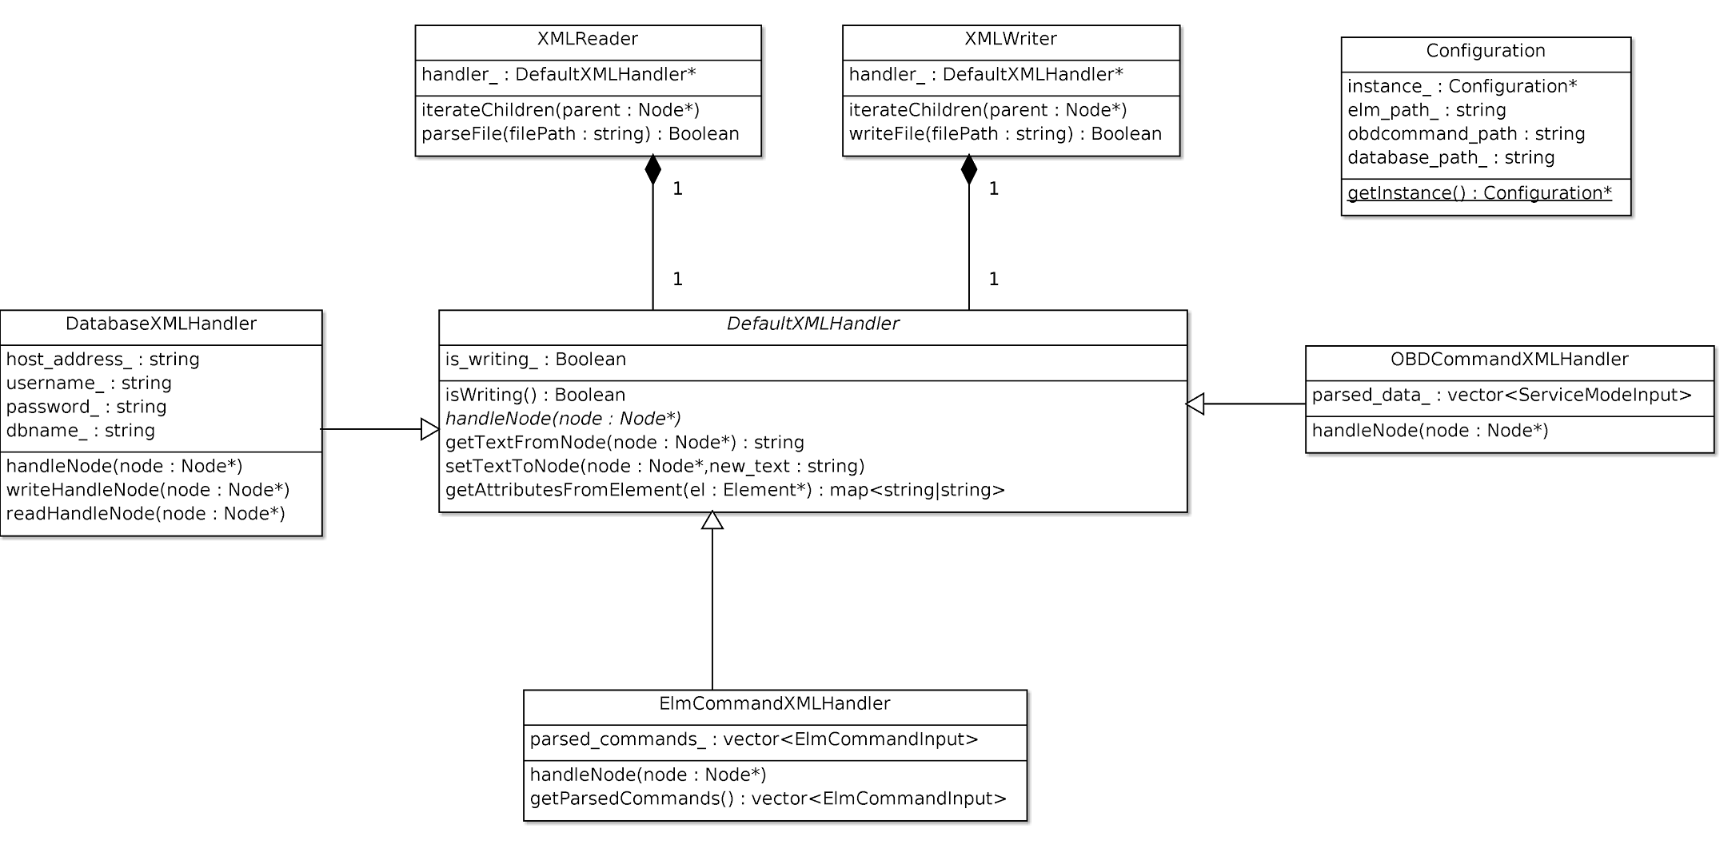
\includegraphics[width=\paperwidth]{figures/classdiagram_configuration}
%  \caption{Classdiagram of the configuration package}
% \end{figure}

%% vim:foldmethod=expr
%% vim:fde=getline(v\:lnum)=~'^%%%%\ .\\+'?'>1'\:'='
%%% Local Variables: 
%%% mode: latex
%%% mode: auto-fill
%%% mode: flyspell
%%% eval: (ispell-change-dictionary "en_US")
%%% TeX-master: "main"
%%% End: 
%%%% Time-stamp: <2012-08-20 17:41:39 vk>

%% example text content
%% scrartcl and scrreprt starts with section, subsection, subsubsection, ...
%% scrbook starts with part (optional), chapter, section, ...

\chapter{Project Specific Implementation}
\label{sec:projectspecific} 

The preceding package implementation descriptions only focus on overlapping functionalities. 
The result is the OBDMiddleware package which is an API.
Furthermore a concrete application has to be implemented to apply the designed features.
The OBDCU, which stands for On Board Diagnosis Control Unit, represents the emulated diagnosis CU.
It offers possibilities to emulate attached USB devices on Linux systems and is able to set and unset
permanent and pending diagnostic trouble codes as well as deleting them.

The OBD tool is supposed to be its counterpart for reading trouble codes and its corresponding freeze frame data,
but since our time contingent did not suffice the OBD tool as well as the OBDCU’s sensor capabilities are not implemented. 
Although it is safe to say that the general functionalities for requesting sensor data is included in the OBDMiddleware. 
Even though the common mechanics are asserted by unit tests,
the additional implementation and connection of the related sensor functions is beyond the scope of this bachelor thesis.

By using CMake simple compilation and dependency requirements can be ensured.
The latter is particularly important, since dependencies on external and internal packages would be difficult to check otherwise.
A setup for development is provided by making paths to the subprojects configurable. 
Packaging for installation is realized by using CPack generators, especially for Debian systems.

The Model-View-Controller architecture is chosen due to its clear specification of classes and their clustering into general divisions. 
The model being represented by the middleware package itself.

\section{OBDCU}

The OBDCU application offers the user the possibility to emulate and partially configure an USB FTDI device with one configuration
and one set of bulk endpoints. Furthermore diagnostic trouble codes are selectable from a database and settable to the emulated 
fault memory either as a permanent or temporary trouble code. 
Additionally it provides a surface to configure responses to ELM commands, where atz.

The current beta version has several restrictions regarding the configurations. They are only kept in memory while the application is running. 
However it is capable of simulating at least three of ten service modes as well as all ELM commands.
As previously mentioned service modes one and two, which represent reading of sensor and freeze frame data, are prepared in the OBDMiddleware package
but since the project has already exceeded the projected time for this bachelor thesis the implementation was skipped.

\section{Installation How-To}

Several steps have to be carried out before starting or building the project on a development environment.
This project has a lot of dependencies, which are listed in the built package, and it requires kernel modules.
This section elaborates on additional dependencies and building instructions depending on the purpose.

The project uses different open source APIs to realize the desired functionalities.
The following packages are included in the official Ubuntu repositories and can be downloaded by any package management system:

\vbox{
\begin{itemize}
 \item libmysqlcppconn-dev 
 \item mysql-server
 \item libusb 
 \item libusb-dev
 \item libxml++2.6-2 
 \item libxml++2.6-2-dev 
 \item qt-sdk
 \item libcppunit-dev 
 \item libcppunit-1.13-0 
 \item libboost-all-dev 
\end{itemize}
}

The only packages which require manual compilation are the libusb-vhci library and the vhci\_hcd package, 
resulting in two kernel module files (.ko). Those files either have to be inserted manually using insmod 
or they have to be installed with the help of ``make install''. When installing and frequently accessing the 
kernel modules it is advisable to alter the modules system file, located under “/etc/modules”, by adding 
them at the end of the file. This will result in the loading of the kernel modules at startup.

To compile the libusb-vhci project the following steps should be taken:

\paragraph{vhci\_hcd}

\begin{enumerate}
 \item download or use from repository
 \item make
 \item sudo make install
\end{enumerate}

Optional - depending on how kernel modules want to be handled:

\begin{enumerate}[resume]
 \item insmod usb-vhci-hcd.ko
 \item insmod usb-vhci-iocifc.ko
\end{enumerate}
 
or:
 
\begin{enumerate}
\setcounter{enumi}{3}
 \item sudo gedit /etc/modules \&
 \item add kernel module names (without extension) to file and save
\end{enumerate}

\paragraph{libusb\_vhci [userspace tools]}

\begin{enumerate}
 \item download or use from repository
 \item ./configure
 \item make
 \item sudo make install
 \item sudo ldconfig -v 
\end{enumerate}

Depending on the Linux kernel version and the current vhci\_hcd and libusb\_vhci versions, 
the compiling procedure may vary. These instructions are extracted from the INSTALL 
files from the repositories. The last installation step is to tell the Linux ld path that 
libusb-vhci has been added to the library path so that it can be included normally.

\section{Building the Project}

When building the OBD project it is essential that it is built in the right order. 
The OBDMiddleware package has to be built before the project specific parts. 
Each part of the OBDMiddleware package can be compiled separately, although it is not advisable, 
since the packages have internal dependencies. 
With the support of CMake building in any location is possible with the command:

\begin{verbatim}
 cmake <path to parent CMakeLists>
\end{verbatim}

Furthermore a package can be built using make package. This will result in a .deb file for Ubuntu distributions. 
Executing the generated file leads to the installation of the files into the library path of the Linux system. 

Like in most software projects it was deemed necessary, that the project can be built with just a compiled version 
of the middleware in case some changes emerge. Thus the project specific parts can be built without parameters 
if the OBDMiddleware package is installed. When intending to use the compiled version it can be built by delivering 
the CMake variable Middleware\_BASE\_PATH.

\begin{verbatim}
 cmake -DMiddleware_BASE_PATH=/home/<...>/OBDMiddleware/build/ .. 
\end{verbatim}

If the path has changed it is advisable to clear the build directory or at least delete the generated CMakeCache.txt 
since CMake has caching issues and does not reevaluate the given variables but rather uses the stored paths. 



%% vim:foldmethod=expr
%% vim:fde=getline(v\:lnum)=~'^%%%%\ .\\+'?'>1'\:'='
%%% Local Variables: 
%%% mode: latex
%%% mode: auto-fill
%%% mode: flyspell
%%% eval: (ispell-change-dictionary "en_US")
%%% TeX-master: "main"
%%% End: 

%%%% Time-stamp: <2012-08-20 17:41:39 vk>

%% example text content
%% scrartcl and scrreprt starts with section, subsection, subsubsection, ...
%% scrbook starts with part (optional), chapter, section, ...
\chapter{Software Development Techniques}
\label{sec:SDT}

When it comes to software engineering one of the most important questions is which software development process 
is the best fit for the particular project requirements. There is a high variety of possible strategies, whereby 
each strategy has its own strengths and weaknesses depending on their field of application. There is no universal 
solution which fits disregarding circumstances. This means some preparation and 
organizational work inside the software team has to be accomplished beforehand. The right software 
has to consider the experience of the software developers, the team size as well as factor in the needs and wishes 
of other stakeholders. It is important to find the most appropriate methodology to satisfy all parties included \cite{BECK}.

Basically software projects can be divided into phases, so called life cycles. The most common life cycles are 
requirements analysis and definition, software design, implementation, verification and maintenance. Taking those 
phases into account a division into two groups evolved: traditional and agile approaches.

Traditional approaches typically execute the phases sequentially, meaning that one phase does not get processed if 
its predecessor has not yet been completed. The waterfall model is considered to be a well-known representative for a traditional approach \cite{WATERFALL},
the basic waterfall model is illustrated in \myfigref{fig:waterfall}.

\myfig{waterfall}%% filename w/o extension in the folder figures
 {width=\textwidth}%% maximum width/height, aspect ratio will be kept
 {Classic Waterfall Development Process \protect{\cite{WATERFALLIMAGE}}}%% caption
 {Figure}%% optional (short) caption for list of figures
 {fig:waterfall}%% label

On the contrary agile approaches are based on iterative and incremental development, which means that the life cycles 
get passed through several times. Thus agile approaches more often result in intermediate software releases which 
encourage adaptations even late in the project’s development phase. Extreme programming is just one of many realisations 
of agile software development methodologies. Since key aspects of its definition are used in the implementation of the OBD 
software its background as well as its approach are covered in this section. 

The following sections layout the reasons for choosing a particular software development technique. 
In addition to that the basics will be explained in particular together with our approach and a final summarization 
containing experiences and knowledge gathered by practicing those methodologies over the course of the bachelor thesis.
The theoretical background is acquired by studying \citeauthor{BECK}'s \citetitle{BECK}\cite{BECK}, \citeauthor{CLEANCODE}'s \citetitle{CLEANCODE}\cite{CLEANCODE} and
\citeauthor{AUTOSPICE}'s \citetitle{AUTOSPICE}\cite{AUTOSPICE}.

\section{Basics}

The motivation to apply the extreme programming methodology is based on the already gathered know-how in this field by attending 
and finishing the course “Softwareentwicklung und Wissensmanagement” in a prior semester. Additionally, taking into consideration 
that the software is designed to be used in an automotive context, the Automotive SPICE\cite{AUTOSPICE} standard, which is derived from the ISO $15504$, 
has to be combined with the test driven development aspect of extreme programming.

Last but not least prioritizing a consistent coding style within the project to keep the source code itself as well as the overall 
structure as clear as possible is intended. Thus simplifying future maintenance and refactoring for programmers who are not implicitly 
the initial developers of the source code. Furthermore this goal is pursued by basically agreeing to an internal coding standard 
based on the book \citetitle{CLEANCODE}\cite{CLEANCODE}.

\subsection{Extreme Programming}
\label{sec:XP}

As mentioned in the previous chapter the extreme programming\cite{BECK} technique falls into the category of agile software development. Generally it is designed 
for small teams to develop software whose requirements change frequently due to their ambiguous definition. Furthermore it is meant 
to be a test driven development approach. In other words a central point of extreme programming is to write unit tests before any ``real'' 
code is written. This promotes the passing of newly written tests as well as already implemented ones. Rather than 
focussing on testing each unit separately, extreme programming also requires to test the whole system, in the best case, several times a day.

Best practice in extreme programming is to perform pair programming, whereas in other software development techniques each developer has an 
own task which needs to be merged in the end. Pair programming is done by two programmers sitting in front of one PC using just one set of 
all required peripherals (screen, keyboard, mouse etc.). Typically, the source code and design of the software gets refactored 
and improved during the whole process for keeping flexibility high and complexity low.

Compared to other software development techniques there are some major differences: First and foremost there is no specialization of the 
developers on a single task, meaning that an XP programmer has to acquire knowledge and new ways of thinking in all parts 
which are related to software development. Starting with analysing requirements over designing the software architecture to programming, 
testing and maintaining the product after each release.

It should be emphasized that analyzing, designing, as well as the developing of infrastructure and frameworks should not be performed 
up-front. Extreme programming takes the view that those steps are done when needed. This leads to a quicker development start as well 
as more qualified decisions, due to gathered experience while dealing with the project. Thus simplifying the estimate of which details 
deserve more attention than others.

Another advice by \citeauthor{BECK} in \citetitle{BECK}\cite{BECK} is to communicate face-to-face or through efficient tests and 
clear code rather than focussing on writing implementation documentation and wasting time with maintaining those documents.

\subsection{Automotive SPICE}

\citetitle{AUTOSPICE}\cite{AUTOSPICE} is a standard used to assess development processes of control unit's software related parts in the automotive industry. It is derived from the 
ISO/IEC $15504$, which is the general SPICE standard, whose main goal is the assessment of processes in software development. SPICE is an 
abbreviation for \textbf{S}oftware \textbf{P}rocess \textbf{I}mprovement and \textbf{C}apability d\textbf{E}termination, which already 
clarifies the principal aims. Automotive SPICE was developed by the AUTOSIG - the \textbf{Auto}motive \textbf{S}pecial \textbf{I}nterest 
\textbf{G}roup, to whom many well known manufacturers belong to, such as Audi, BMW, Fiat, Jaguar and a few more.

Generally the \citetitle{AUTOSPICE}\cite{AUTOSPICE} Process Assessment Model (PAM) can be described as a two-dimensional model consisting of a process dimension 
and a capability dimension. The process dimension defines several process categories, where processes are grouped depending on their type of 
activity. The capability dimension is composed of capability levels, which contain sets of process attributes who provide the measurable 
characteristics of process capability.

The process dimension is described by the Automotive SPICE Process Reference Model (PRM). Thereby three process categories are defined: Primary life
cycle processes, organizational life cycle processes and supporting life cycle processes. Each category is divided into process groups.

The primary life cycle processes category entails an acquisition process group (ACQ), a supply process group (SPL) and an engineering process 
group (ENG). Each group is then described by several processes in detail. ACQ processes are used by the customer as well as the supplier in 
order to acquire a product or a service. SPL processes are meant for the supplier to actually supply a product or a service. ENG processes 
cover the handling of customer requirements defined in the ACQ process as well as the specification, implementation and maintaining of the 
software product and its relation to the system.

The supporting life cycle processes category consists only of one support process group (SUP) whose processes can be employed by the other processes at any time.

Lastly the organizational life cycle processes category includes a management process group (MAN), a process improvement process group (PIM) 
and a reuse process group (REU). MAN processes describe practices to manage projects or processes. PIM processes deal with defining, deploying 
and improving processes. REU processes systematically exploit opportunities in organization’s reuse programs.

\citetitle{AUTOSPICE}\cite{AUTOSPICE} includes the capability dimension which describes six capability levels as following:

\vbox{
\begin{itemize}
 \item Level 0 - Incomplete process:
 \begin{itemize}
  \item Process is not implemented or fails to achieve its purpose. At this level there is little or no evidence of any systematic achievement of the process purpose.
 \end{itemize}

 \item Level 1 - Performed process:
 \begin{itemize}
  \item The implemented process achieves its process purpose.
 \end{itemize}
 
 \item Level 2 - Managed process:
 \begin{itemize}
  \item The previously described performed process is now implemented in a managed fashion (planned, monitored and adjusted) and its work products are appropriately established, controlled and maintained.
 \end{itemize}
 
 \item Level 3 - Established process:
 \begin{itemize}
  \item The previously described managed process is now implemented using a defined process that is capable of achieving its process outcomes.
 \end{itemize}
 
 \item Level 4 - Predictable process:
 \begin{itemize}
  \item The previously described established process now operates within defined limits to achieve its process outcomes.
 \end{itemize}
 
 \item Level 5 - Optimizing process:
 \begin{itemize}
  \item The previously described predictable process is continuously improved to meet relevant current and projected business goals.
 \end{itemize}
\end{itemize}}

\subsection{Clean Code}
\label{sec:CleanCode}

Clean code cannot be considered as a software development technique by itself. It is rather a common guideline for the whole 
software development process. According to this, a programmer who is facing the task of developing new software, should rather prioritize on 
producing clean code from the beginning than valuing speed and coding sloppily.

Referring to \citetitle{CLEANCODE}\cite{CLEANCODE} there is no unique definition of clean code. It is more likely that every programmer has an own point of 
view when it comes to this question. Thus there are several definitions which overlap partly as well as other ones which diverge widely. 
An appropriate definition of clean code is coherent code, which is characterized by making sense to a non familiar reader in a short period 
of time. The reader should not be forced to put too much effort into trying to decrypt the intention behind the code. Clean code also offers 
some advantages. Source code which is written clean is more likely to be more stable. In addition to that maintaining clean code is basically 
much more efficient when it comes to expanding or debugging.

In addition to code conventions and design patterns, which are depending on an agreement within a software developing team, there is a set of rules
which can be followed to enhance code readability according to \citeauthor{CLEANCODE}.

\myfig{mindmap_clean_code}%% filename w/o extension in the folder figures
 {width=\textwidth}%% maximum width/height, aspect ratio will be kept
 {Clean Code Mindmap}%% caption
 {Figure}%% optional (short) caption for list of figures
 {fig:clean_code}%% label

\myfigref{fig:clean_code} visualizes the most important clean code concepts concerning this project. The mind map reveals the basic 
idea behind clean code with high information density. The following paragraphs are describing each clean code feature a little more detailed
including some examples to clarify its intention.

Intention-revealing names are recommended, as the name of a function, class or variable should 
be self-explaining, diminishing the need for descriptive comments. Any chance of improving the naming should be taken. Calling a variable 
timeSinceFirstExecution is more illuminating than single letter variables like x, y or abbreviations such as tsfe. This also directly 
covers the subitems ``avoid disinformation'', ``meaningful distinctions'' and ``pronounceable and searchable names''. In practice the 
usage of uppercase ``o'' or lowercase ``L'' is considered as bad naming due to their similarity with ``$0$'' and ``$1$''.
It is recommended to use nouns for class names and verbs for method naming.

Keeping functions as small as possible, meaning that a function consists only of a few lines without being in need of complex 
nested structures, has the advantage of making them more readable and understandable. Therefore methods should exclusively implement a single functionality, 
neglecting all other circumstances. As highlighted in the earlier paragraph function names should describe the intended purpose of the function as detailed as possible. 
Unnecessary code duplication is avoided by encapsulating recurring code into separate functions.

Due to the nature of comments, describing complicated and unorganized code, it is preferable to have as few comments as possible.
Since comments are considered a sign for programmer laziness, it is better to invest some time into refactoring the naming of variables
and functions rather than placing a comment. Nevertheless good comments exist as well like empty catch-blocks. Further examples can be looked up in 
\citetitle{CLEANCODE}\cite{CLEANCODE}.

Executing code formatting is also part of the clean code philosophy, thus enhancing the general readability of the code as well as simplifying 
it for future maintenance. There are some recommendations for both vertical and horizontal formatting, as for instance splitting concepts in 
such a way that closely associated code parts are vertically dense. Same goes for the horizontal formatting, where a certain spacing hints at 
relations and separations. Furthermore indentations should be used to hierarchically separate different scopes.

The chapter ``Unit Tests'' highly influenced the software development as extreme programming is built upon unit testing 
and test driven development. There is a set of three rules concerning test driven development besides the already mentioned priority of writing 
and executing tests before code is actually implemented:

\begin{enumerate}
 \item ``You may not write production code until you have written a failing unit test.''
 \item ``You may not write more of a unit test than is sufficient to fail, and not compiling is failing.''
 \item ``You may not write more production code than is sufficient to pass the currently failing test.''
\end{enumerate}

It is important to maintain tests as well as the tested code clean. Clean tests should be designed in such a manner that they obey the “F.I.R.S.T.” principle, 
which is an acronym of five rules:

\begin{description}
 \item [F]ast - meaning tests run quickly so they get executed frequently.
 \item [I]ndependent - tests do not influence each other
 \item [R]epeatable - they conclude to the same result in any environment
 \item [S]elf-validating - returning only by a boolean output whether a test passes or fails, no additional log files which lead to confusion
 \item [T]imely - writing a test takes place just right before writing the real code to reduce the risk of untestable code
\end{description}

Concluding classes and functions should be as small as possible. As opposed to functions the shortness is not measured in lines of code, but 
rather in the amount of class responsibilities. This leads to the so called single responsibility principle which purports that classes or modules 
should have only one reason to change. Additionally they should be prepared for code changes and without obvious structure to avoid complicated workarounds
or program crashes.

\section{Realization}

The scientific aspect of this bachelor thesis is focused on the combination of agile software development in the automotive context. The 
foundation of this approach builds the Automotive SPICE PAM (PRM) model as well as elements from \citeauthor{BECK} \citetitle{BECK}. 
This chapter will describe the design of combining these software development processes, techniques and tools, which restrictions  
and compromises are made. The following chapter \nameref{sec:conclusion} is then a subjective summary of experiences and insights.

The chosen software is in the vicinity of automotive software development but still for users with little to no automotive knowledge. 
Automotive software development often falls into the category of safety-critical systems, which have high 
security and low fault tolerance criteria as well as strict and complex testing requirements of its software with severe consequences of failure.

However safety uncritical systems, like average software, have their focus on usability and visual representation as well as extendability and 
effectiveness. Since this software belongs to two areas of software development, the conclusion lies near that the development techniques 
from both areas have valid ground for application. 
Therefore it is necessary to design a combined development technique by picking the most suitable processes of each technique. 
Starting with the ACQ 
processes from the SPICE development technique set, customer/system requirements are defined.

\begin{tabular}{| c | p{12cm} |}
 \hline
 \textbf{Module} & \textbf{We want an OBD tool...} \\
  \hline
  1 & that is free of charge. \\
  \hline
  2 & whose source code is available. \\
  \hline
  3 & which can read and reset DTCs. \\
  \hline
  4 & with which we can see online sensordata. \\
  \hline
  5 & which is usable through USB interface. \\
  \hline
  6 & whose usability is adapted to the target group. \\
  \hline
  7 & which is easily extendable. \\
  \hline
  8 & which conforms the WWH-OBD and European OBD standards. \\
  \hline
  9 & which is usable with a range of OBD-HW or easily extendable to third party hardware. \\
  \hline
  10 & which can be tested without any hardware. \\
  \hline
\end{tabular}

The next step according to SPICE is to parse those customer requirements to software and hardware requirements. The latter are simple, since 
this project only requires an average ELM$327$. The software requirements, on the other hand, are designed quite thoroughly.

% LANDSCAPE FUNCTIONAL REQUIREMENTS

The detailed design, which is the next task, results in the first compromis. It seems smart to move the detailed design of each package 
to right before implementing it. This corresponds to agile software development requirement of doing the design of the task to implement as late 
as possible.

The implementation of the packages is done by using the following agile software development techniques:

\begin{itemize}
 \item Test Driven Development
 \begin{itemize}
  \item trust into the produced code
 \end{itemize}

 \item Pair Programming
 \begin{itemize}
  \item resulting in less time to search bugs
 \end{itemize}
 
 \item Constant Refactoring
 \begin{itemize}
  \item resulting in code resistance and no functionality duplication
 \end{itemize}
\end{itemize}

Since the rough design and thus the order in which the single functionalities have to be implemented is already defined by the SPICE processes,
agile software development for the single packages can easily be applied. Although this approach breaks the premise of agile software 
development to have as little design overhead as possible, but instead doing the design when implementing, it seems to be a valid compromise to 
merge the SPICE PRM with the techniques of agile software development. 

Summarized, the approach can be interpreted as a merge of the SPICE PRM advantages, and the freedom 
and scalability of agile software development. The difference to the classic SPICE model is including the execution order of certain processes, 
like detailed design. Furthermore the comparison to the requirements is not tested at the completion of the project, but rather defined before 
even beginning programming, through the unit tests. Agile software development differs from its classical approach by taking some flexibility 
through the division into packages at the ACQ phase of the SPICE models. All in all the approach seems valid especially for this kind of 
software and is tested out by implementing code in that certain area as well. A further description of the gained insights can be found in the 
\nameref{sec:conclusion} chapter.

%% vim:foldmethod=expr
%% vim:fde=getline(v\:lnum)=~'^%%%%\ .\\+'?'>1'\:'='
%%% Local Variables: 
%%% mode: latex
%%% mode: auto-fill
%%% mode: flyspell
%%% eval: (ispell-change-dictionary "en_US")
%%% TeX-master: "main"
%%% End: 


%% include tex file chapters:
% \include{introduction}        %% this is a suggestion: you have to create this file on demand
% \include{problem}             %% this is a suggestion: you have to create this file on demand
% \include{solution}            %% this is a suggestion: you have to create this file on demand
% \include{evaluation}          %% this is a suggestion: you have to create this file on demand
% \include{outlook}             %% this is a suggestion: you have to create this file on demand

\appendix                       %% closes main document, appendix follows until end; only available in book-classes
\addpart*{Appendix}             %% adding Appendix to tableofcontents

\printbibliography              %% remove, if using BibTeX instead of biblatex
% \include{further_ressources}  %% this is a suggestion: you have to create this file on demand

%%%% end{document}
\end{document}
%% vim:foldmethod=expr
%% vim:fde=getline(v\:lnum)=~'^%%%%\ .\\+'?'>1'\:'='
%%% Local Variables:
%%% mode: latex
%%% mode: auto-fill
%%% mode: flyspell
%%% eval: (ispell-change-dictionary "en_US")
%%% TeX-master: "main"
%%% End:
